% !TeX spellcheck = pl_PL
\documentclass[a4paper,twoside]{article}
\usepackage{polski}
\usepackage[utf8]{inputenc}
\usepackage{graphicx}
\usepackage{amsmath}

\usepackage[unicode, bookmarks=true]{hyperref} %do zakładek
\usepackage{tabto} % do tabulacji
\NumTabs{6} % globalne ustawienie wielkosci tabulacji
\usepackage{array}
\usepackage{multirow}
\usepackage{array}
\usepackage{dcolumn}
\usepackage{bigstrut}
\usepackage{color}
\usepackage[usenames,dvipsnames]{xcolor}
\usepackage{svg}
\usepackage{xfrac}
\usepackage{floatrow}
% Table float box with bottom caption, box width adjusted to content
\newfloatcommand{capbtabbox}{table}[][\FBwidth]
\usepackage{blindtext}


\setlength{\textheight}{24cm}
\setlength{\textwidth}{15.92cm}
\setlength{\footskip}{10mm}
\setlength{\oddsidemargin}{0mm}
\setlength{\evensidemargin}{0mm}
\setlength{\topmargin}{0mm}
\setlength{\headsep}{5mm}

\newcolumntype{M}[1]{>{\centering\arraybackslash}m{#1}}
\newcolumntype{N}{@{}m{0pt}@{}}

\graphicspath{ {./images/} }

% === Reset inkrementacji sekcji przy nowym parcie === %
\usepackage{titlesec}

\makeatletter
\@addtoreset{section}{part}
\makeatother
\titleformat{\part}[display]
{\normalfont\LARGE\bfseries\centering}{}{0pt}{}

\begin{document}
\bibliographystyle{plain}



\begin{titlepage}
\title{\huge Sieci Komputerowe - ULTIMATE}
\author{\large SonMati}
\maketitle
\end{titlepage}

\newpage

% === TEORIA
% !TeX spellcheck = pl_PL

\part{Protokół komunikacyjny}
	Jest to mechanizm, który służy do wymiany informacji pomiędzy dwiema stacjami, jednostkami cyfrowymi (\emph{DD - digital device}). 
	\section{Skład protokołu}
		\begin{itemize}
			\item Synchronizacja kooperacji
			\item Role obu obojga (\emph{parties})
			\begin{itemize}
				\item Peer to Peer (P2P)
				\item Master-Slave
			\end{itemize}
			\item \emph{Framing} (Ramkowanie, format przesyłanych danych)
			\item Poprawa błędów
		\end{itemize}
	\section{Enkapsulacja}
		\subsection{5 warstw}
			\begin{table}[h]
				\begin{tabular}{|c|}
					\hline
					Aplikacja        \\ \hline
					Transport        \\ \hline
					Sieć             \\ \hline
					Link access      \\ \hline
					Fizyczna warstwa \\ \hline
				\end{tabular}
			\end{table}
		\subsection{3-poziomowa architektura komunikacji}
			\begin{itemize}
				\item File transfer $\longleftrightarrow$ File transfer (Transport, Aplikacja)
				\item Transport $\longleftrightarrow$ Transport (Sieć)
				\begin{itemize}
					\item Transport właściwy
					\item Sieć (Network)
				\end{itemize}
				\item Network Access $\longleftrightarrow$ Communication network
				 $\longleftrightarrow$ Network Access (Link access)
				 \begin{itemize}
				 	\item Logiczne połączenie (Link Access)
				 	\item Fizyczne połączenie (Physical Access)
				 \end{itemize}
			\end{itemize}
	\section{Service Access Point (SAP)}
		SAP jest wykorzystywany w sieciach typu OSI (\emph{Open Systems Interconnection}), jest to etykietę identyfikująca dla punktów końcowych sieci. Innymi słowy, oznacza ich lokalizację w sieci.
		\subsection{Format}
		\begin{table}[h]
			\begin{tabular}{|c|c|c|c|c|}
				\hline
				Nagłówek & Host & Punkt przeznaczenia & Dane & Kontrola błędów \\ \hline
			\end{tabular}
		\end{table}
		Kolejność wykonywania wiadomości w protokole:
		\begin{table}[h]
			\begin{tabular}{|c|l|}
				\hline
				Aplikacja	& Dane								\\ \hline
				Transport	& Punkt przeznaczenia + Dane		\\ \hline
				Sieć		& Host + Punkt przeznaczenia + Dane	\\ \hline
				Link access & Nagłówek + Host + Punkt przeznaczenia + Dane + Kontrola błędów \\ \hline
			\end{tabular}
		\end{table}
		Przykład sieci:\\
		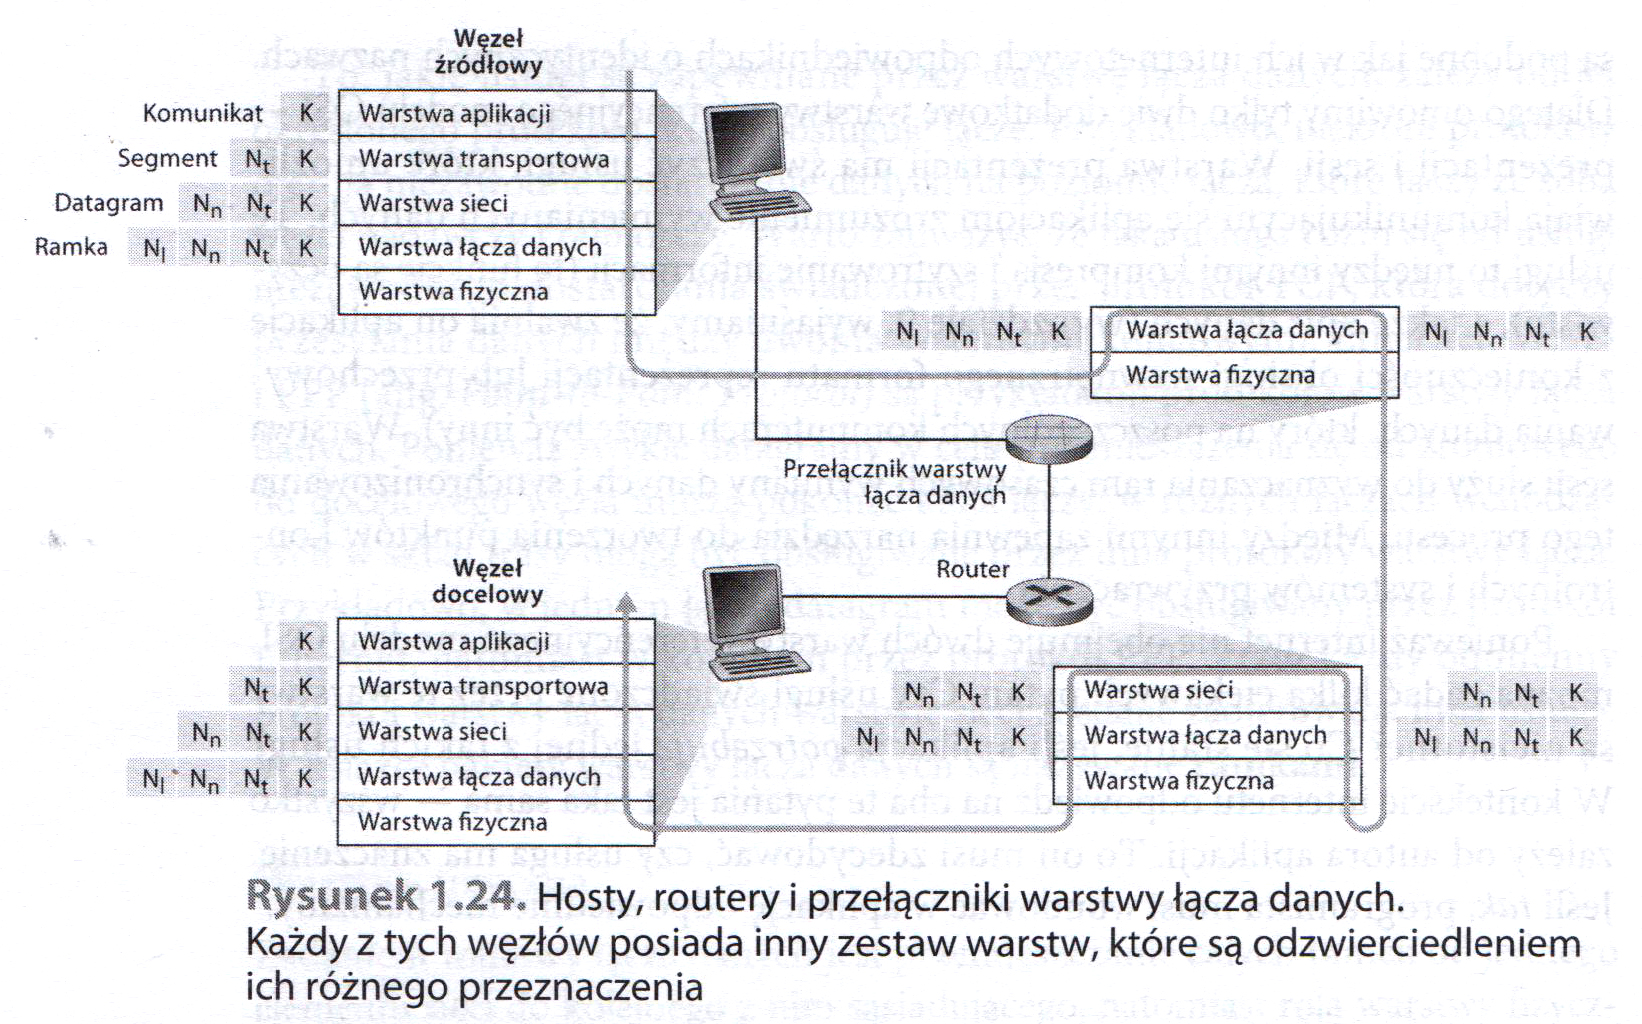
\includegraphics[width=11cm]{./images/image01.jpg}

\part{Model ISO / OSI}
	\section{7-warstwowy model}
		Jest to tzw. \textbf{stos protokołów}, zaprezentowany od "góry do dołu".
		\begin{table}[h]
			\begin{tabular}{|c|}
				\hline
				Warstwa aplikacyjna	\\ \hline
				Warstwa prezentacyjna	\\ \hline
				Warstwa sesji		\\ \hline
				Warstwa transportowa		\\ \hline
				Warstwa sieci	\\ \hline
				Warstwa łącza danych		\\ \hline
				Warstwa fizyczna \\ \hline
			\end{tabular}
		\end{table}
		Każda warstwa świadczy pewne usługi warstwie znajdującej się ponad nią. Innymi słowy, warstwa korzysta z usług tej bezpośrednio poniżej.
		\begin{itemize}
			\item \textbf{Warstwa aplikacyjna}
			\begin{itemize}
				\item Zapewnia dostęp do środowiska OSI dla użytkownika
				\item Udostępnia usługi informacyjne
				\item Pakiety w tej warstwie nazywamy \textbf{komunikatami}
			\end{itemize}
			\item \textbf{Warstwa prezentacyjna}
			\begin{itemize}
				\item Zapewnia niezależność procesom aplikacji od różnic w prezentacji danych (składnia), czyli spełnia rolę tłumacza.
				\item Jej zadaniem jest świadczenie usług, które umożliwiają komunikującym się aplikacjom zrozumienie wymienianych danych, m.in. kompresja, opis i szyfrowanie danych
				\item Na tym poziomie następuje enkrypcja (szyfrowanie) danych
			\end{itemize}  
			\item \textbf{Warstwa sesji}
			\begin{itemize}
				\item Zapewnia kontrolę struktury dla komunikacji między aplikacjami
				\item Ustanawia, zarządza i kończy połączenie (sesję) pomiędzy współpracującymi aplikacjami
				\item Służy do wyznaczania ram czasowych wymiany danych i synchronizowania tego procesu
				\item Umożliwia tworzenie punktów kontrolnych i systemów przywracania.
			\end{itemize}
			\item \textbf{Warstwa transportowa}
			\begin{itemize}
				\item Zapewnia niezawodny, przejrzysty transfer danych pomiędzy punktami końcowymi
				\item Zapewnia "od końca do końca" poprawę błędów i sterowanie przepływem.
				\item Pakiety w tej warstwie nazywamy \textbf{segmentami}.
				\item Przykłady: TCP, UDP
			\end{itemize}
			\item \textbf{Warstwa sieci}
			\begin{itemize}
				\item Odpowiada za ustawienie, utrzymanie i zakończenie połączenia
				\item Protokół warstwy transportowej hosta źródłowego przekazuje segment i adres docelowy  warstwie sieci
				\item Umożliwia dostarczenie segmentu do warstwy transportowej docelowego hosta
				\item Pakiety w tej warstwie nazywamy \textbf{datagramami}.
			\end{itemize}
			\item \textbf{Warstwa łącza danych}
			\begin{itemize}
				\item Zapewnia niezawodny transfer informacji przez fizyczne łącze
				\item Wysyła bloki (\emph{frames}) z niezbędną synchronizacją, kontrolą błędów i kontrolą / sterowaniem przepływem
				\item Przesyła datagram za pośrednictwem serii routerów
				\item Pakiety w tej warstwie nazywamy \textbf{ramkami}
			\end{itemize}
			\item \textbf{Warstwa fizyczna}
			\begin{itemize}
				\item Dotyczy transmisji niestrukturyzowanego strumienia bitów na fizycznym medium
				\item Dotyczy właściwości mechanicznych, elektrycznych, funkcjonalnych i proceduralnych
				\item Jej zadaniem jest przesyłanie poszczególnych bitów ramki pomiędzy dwoma węzłami
			\end{itemize}
		\end{itemize}
		W zwykłym 5-warstwowym modelu odpowiadające mu warstwy spełniają prawie że te same role.
	\section{Architektura OSI jako Framework}
		\textbf{Wspólny język}: ASN-1 (\emph{Abstract Syntax Notation-One}).\\
		\begin{table}[h]
			\begin{tabular}{|c|lcll}
				\cline{1-1}
				Warstwa 7 &                       & Usługa do warstwy N+1          &  &                                   \\ \cline{1-1}
				...       &                       & $ \updownarrow $                   &  &                                   \\ \cline{1-1} \cline{3-3}
				Warstwa N & \multicolumn{1}{l|}{$ \rightarrow $} & \multicolumn{1}{c|}{Warstwa N} & $ \longleftrightarrow $  & Protokół z rówieśniczą warstwą N \\ \cline{1-1} \cline{3-3}
				...       &                       & $ \updownarrow $                   &  &                                   \\ \cline{1-1}
				Warstwa 1 &                       & Usługa do warstwy N-1          &  &                                   \\ \cline{1-1}
			\end{tabular}
		\end{table}
		Model ISO / OSI wykorzystywany jest w technologiach:\\
		\begin{itemize}
			\item TCP/IP
			\item LAN
			\item MAIL
			\item HTTP
			\item SECURITY
		\end{itemize}


\part{Transfer danych}
	Interesuje nas model \textbf{niezawodnego} transferu danych (\emph{reliable data transfer}). Odgrywa on kluczową rolę w pracy sieci, wykorzystywany jest w warstwie transportowej, łącza danych i aplikacji.\\
	Niezawodny kanał zapewnia, że żadne dane nie są uszkadzane, gubione oraz są dostarczane w tej samej kolejności w jakiej zostaną wysłane. Taki transport danych zapewnia np. protokół TCP.\\
	Idea jest prosta, natomiast trudna i złożona jest \textbf{implementacja} takiego protokołu.\\
	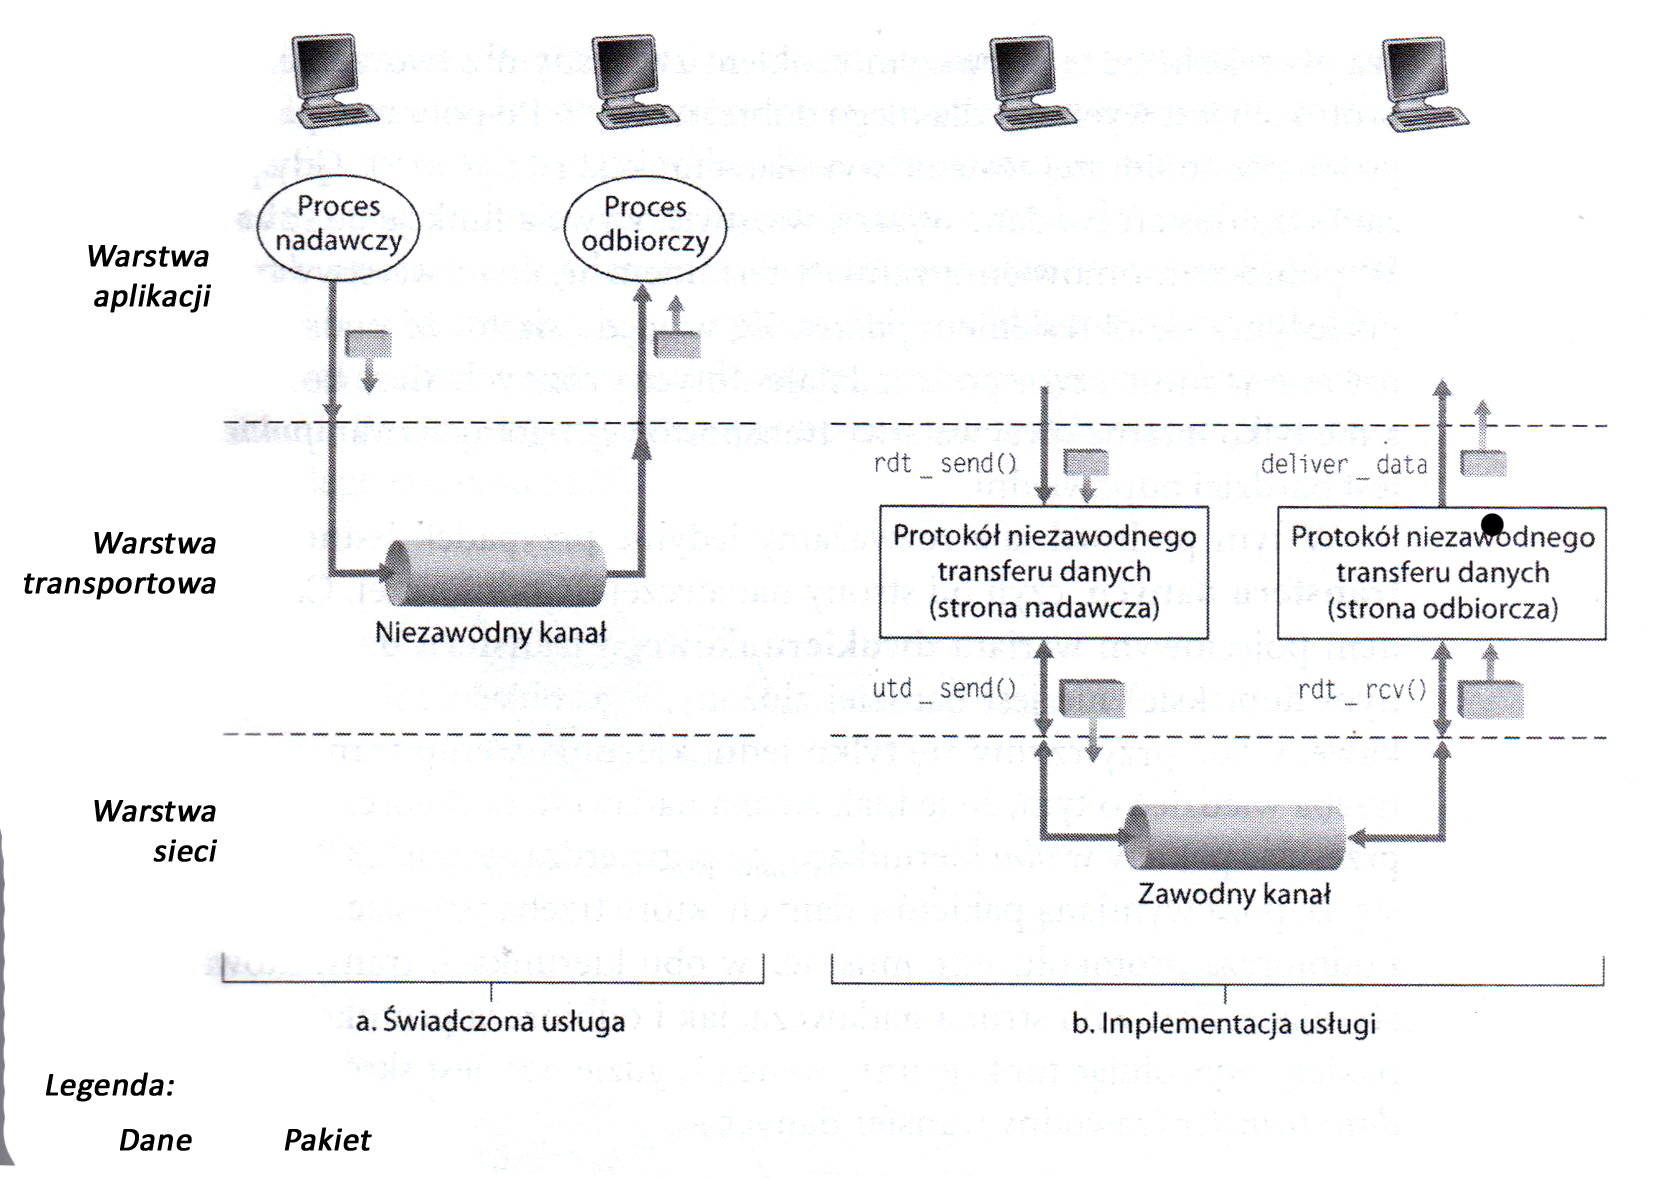
\includegraphics[width=10cm]{./images/image02.jpg}
	\section{Diagramy sekwencji czasowej dla prostych usług}
		\subsection{Potwierdzona / niepotwierdzona usługa}
			Prosty transport danych z punktu widzenia warstwy aplikacji.\\
			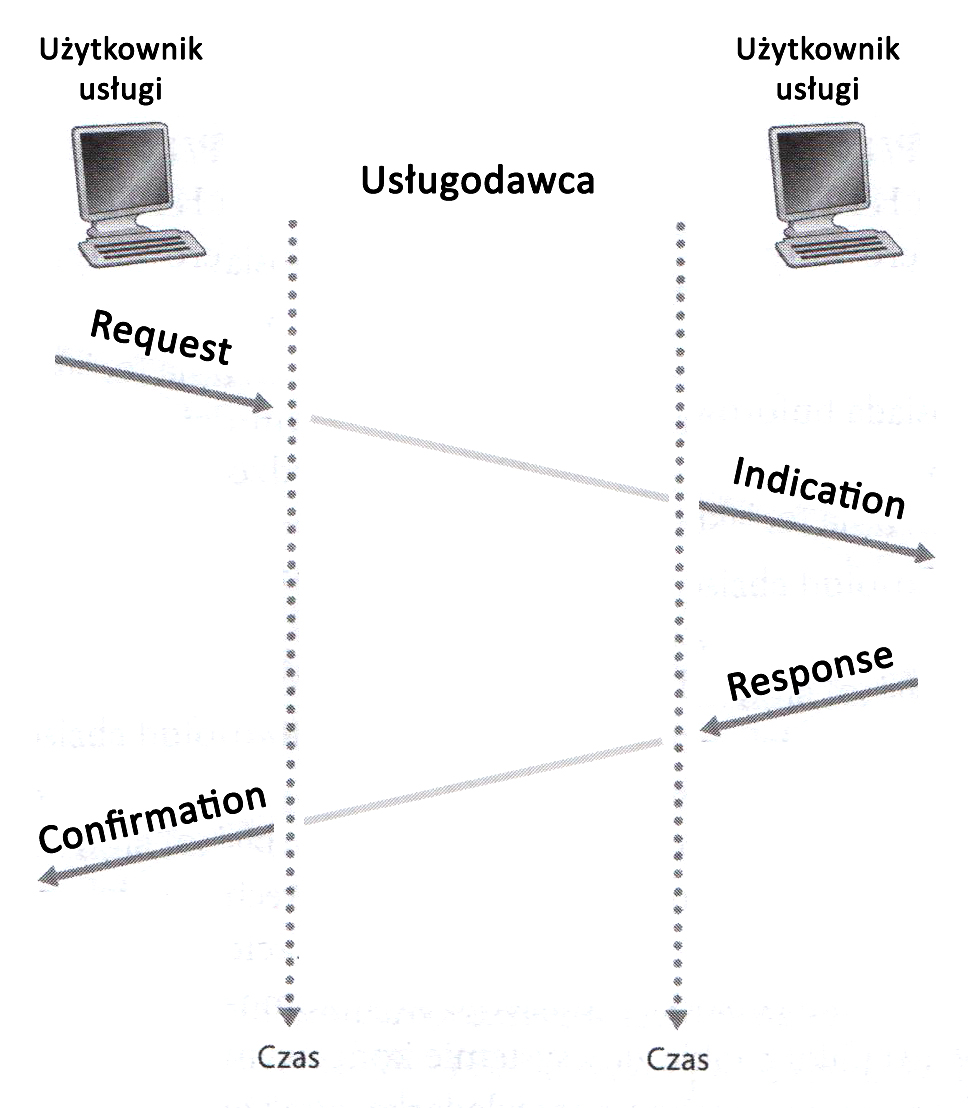
\includegraphics[width=7cm]{./images/image03_confirmation.jpg}
			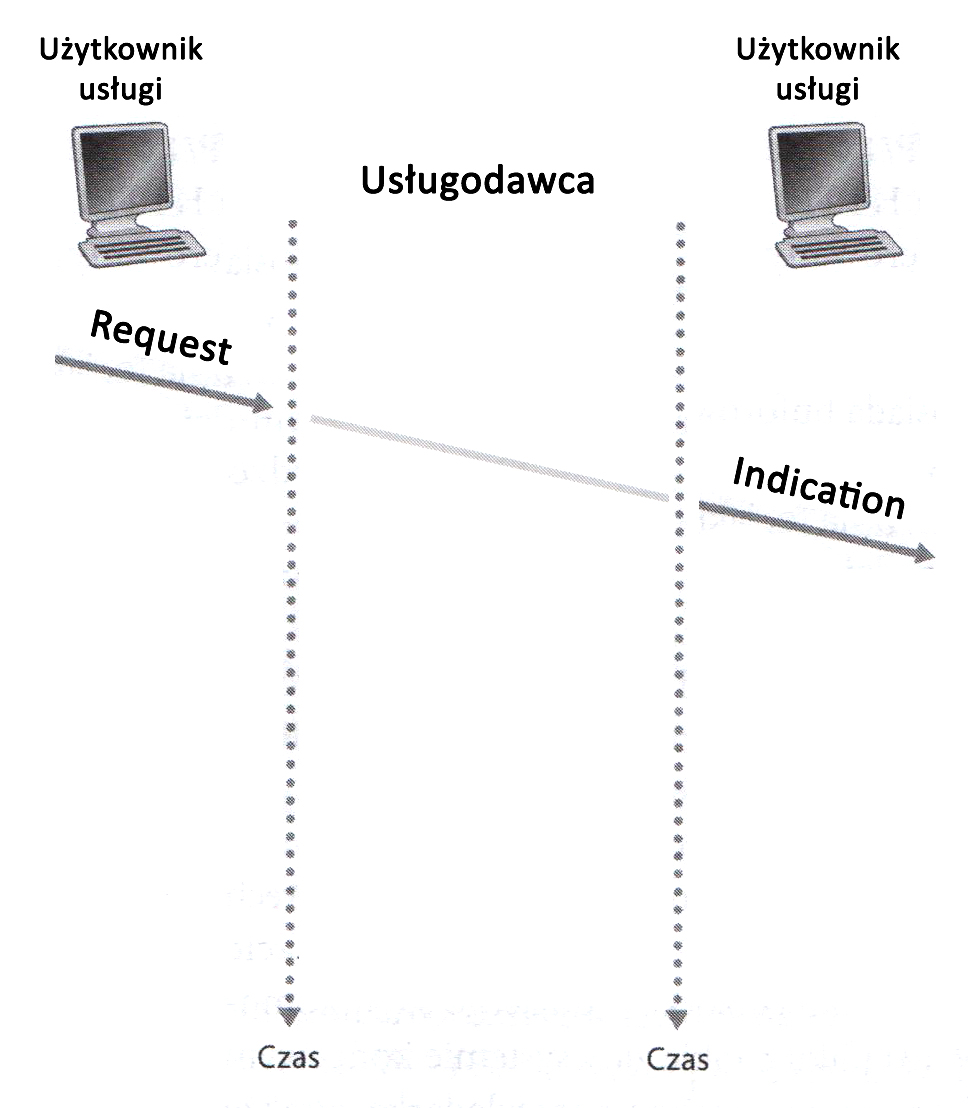
\includegraphics[width=7cm]{./images/image03_no_confirmation.jpg}\\
			Widzimy tutaj \textbf{jednokierunkowy transfer danych} (\emph{half-duplex transfer}) - w danej chwili możliwe jest wyłącznie przesył ze strony nadawczej do odbiorczej.
		\subsection{Wersja z wcześniejszym powrotem}
			Pełny dwukierunkowy transfer (\emph{Full two-way service})\\
			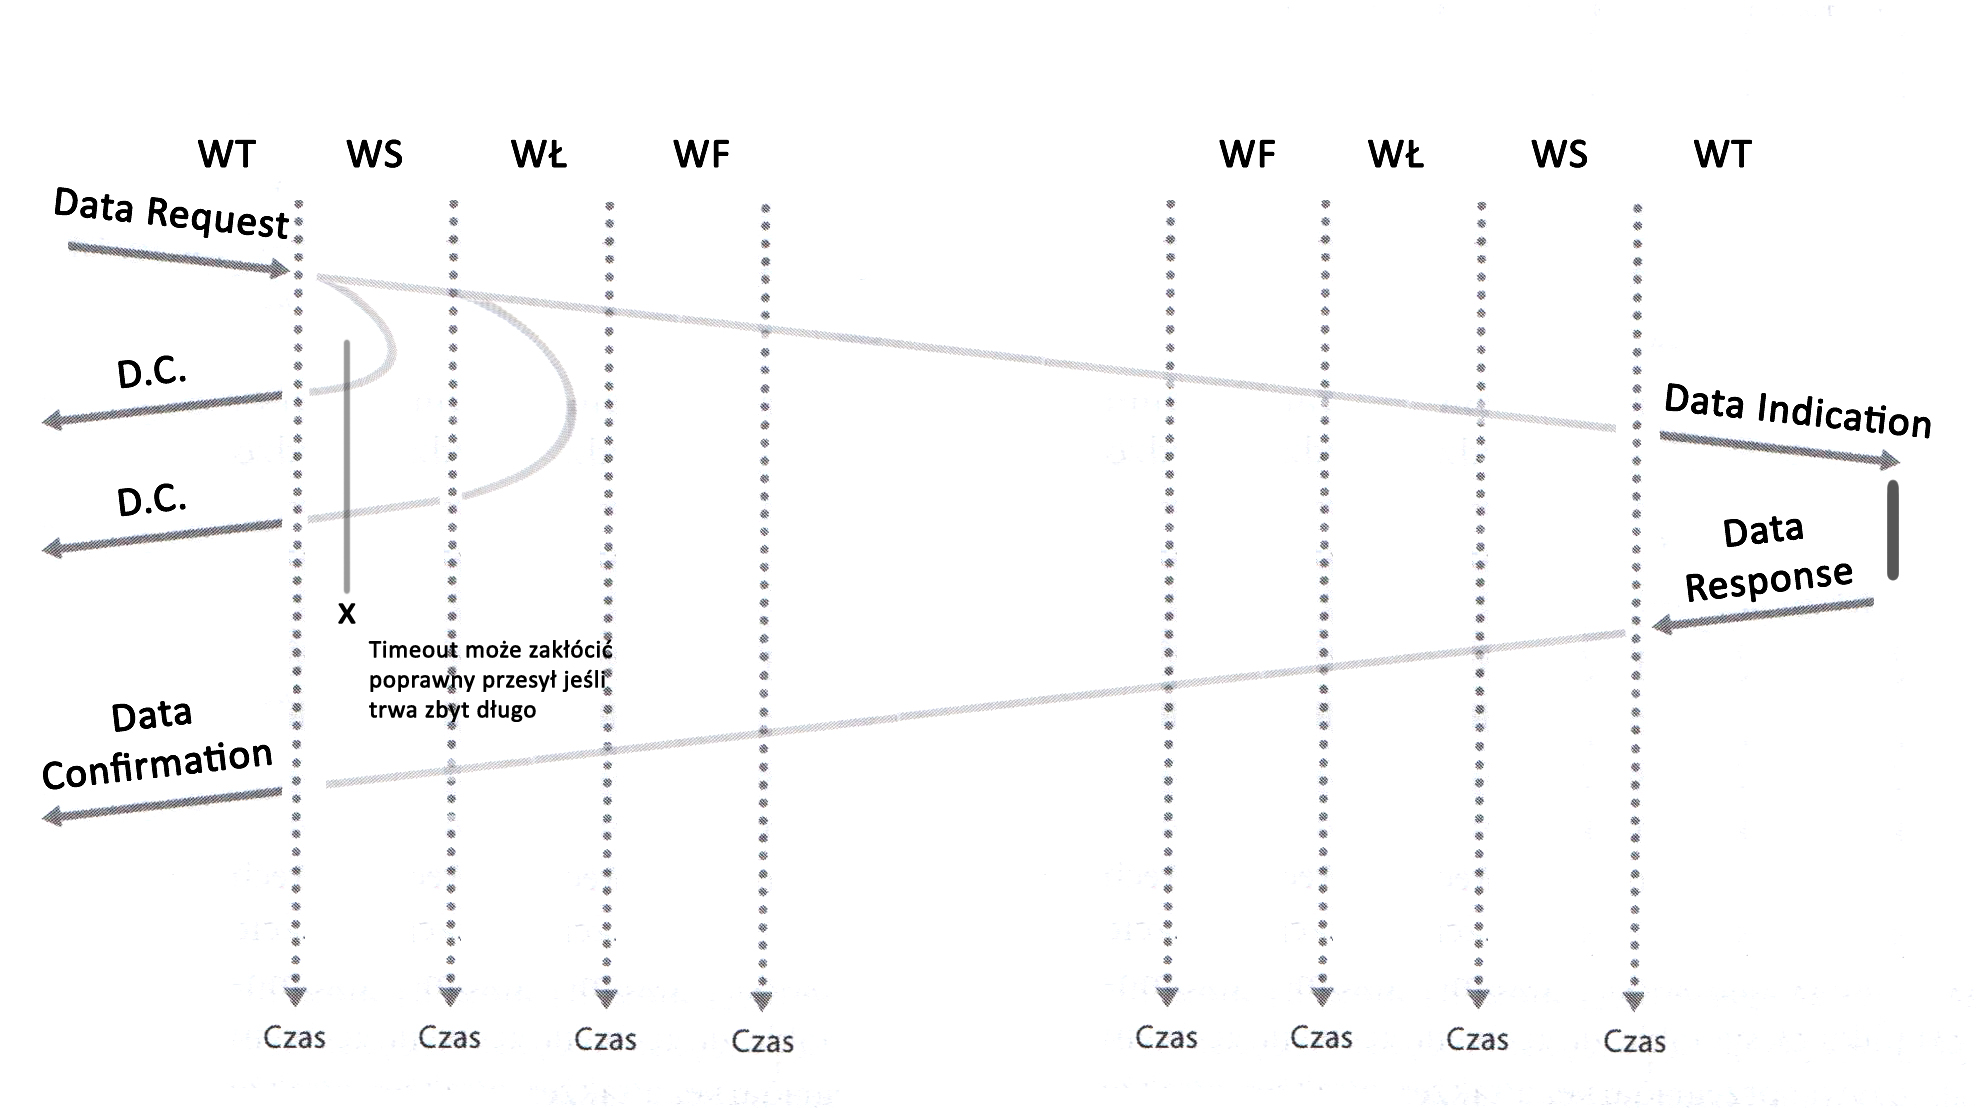
\includegraphics[width=10cm]{./images/image04.jpg}\\
			Nie jest wiele bardziej złożony od jednokierunkowego
	\section{Protokoły}
		Wykorzystujemy je do transferu danych pomiędzy warstwami i dzielimy na:
		\begin{itemize}
			\item \textbf{Znakowe} - przesyłane są pakiety danych
			\item \textbf{Binarne} - przesyłany jest bit po bicie
		\end{itemize}


\part{Binarna komunikacja synchroniczna (BSC)}
	Jest to odmiana protokołu znakowego, który służy do implementacji niezawodnego transferu danych z obsługą błędów występujących w kanale zawodnym.\\
	Protokół wykorzystuje mechanizm potwierdzeń.
	\begin{itemize}
		\item \textbf{Pozytywnych} - poprawna transmisja
		\item \textbf{Negatywnych} - prośba o powtórzenie
	\end{itemize}
	Aby móc obsłużyć błędny transfer protokół musi mieć zaimplementowane dodatkowe funkcje:
	\begin{itemize}
		\item \textbf{Detekcja błędów} - umożliwienie sprawdzenia u odbiorcy czy wystąpiły w błędne bity.
		\item \textbf{Interakcje ze strony odbiorcy} - w przypadku błędnego pakietu odbiorca musi skierować odzew do nadawcy. przykładem są właśnie pozytywne i negatywne potwierdzenia.
		\item \textbf{Retransmisja} - błędny transfer jest ponownie transmitowany.
	\end{itemize}
	\section{Znaki kontrolne}
		Do realizacji zadań stawianych protokołowi BSC wykorzystano poniższą listę znaków kontrolnych:
		\begin{itemize}
			\item \textbf{STX} - Start of Text (początek tekstu)
			\item \textbf{SOH} - Start of Header (początek nagłówka)
			\item \textbf{ENQ} - Enquiry (zapytanie, np. do żądania odpowiedzi)
			\item \textbf{ETX} - End of Text (koniec tekstu)
			\item \textbf{EOT} - End of Transmission (koniec transmisji)
			\item \textbf{ACK} - Acknowledgement (potwierdzenie pozytywne)
			\item \textbf{NAK} - Negative Acknowledgement (potwierdzenie negatywne)]
			\item \textbf{SYN} - Synchronous Idle (czekanie, przed innymi 2 razy)
			\item \textbf{DLE} - Data Link Escape ()
			\item \textbf{ETB}
		\end{itemize}
		Najważniejszymi znakami kontrolnymi są ACK oraz NAK - nasze algorytmy muszą tak kontrolować te komendy, by przesył był poprawny i jak najbardziej efektywny.
	\section{Format danych}
		\begin{table}[h]
			\begin{tabular}{|c|c|c|c|c|c|c|c|}
				\hline
				SYN	&	SYN	&	SOH	&	Nagłówek	&	STX	& Tekst	&	ETX	&	BCC\\ \hline
			\end{tabular}
		\end{table}
	\section{Protokół komunikacji}
		Protokół BSC oparty jest o definicje automatów stanów skończonych (\emph{Finite-State Machine} - FSM) dla strony nadawczej i odbiorczej. Warto zauważyć, że dla obu stron istnieją \textit{niezależne} systemy FSM.
	\section{Schematy żądań}
		\subsection{Odbioru}
			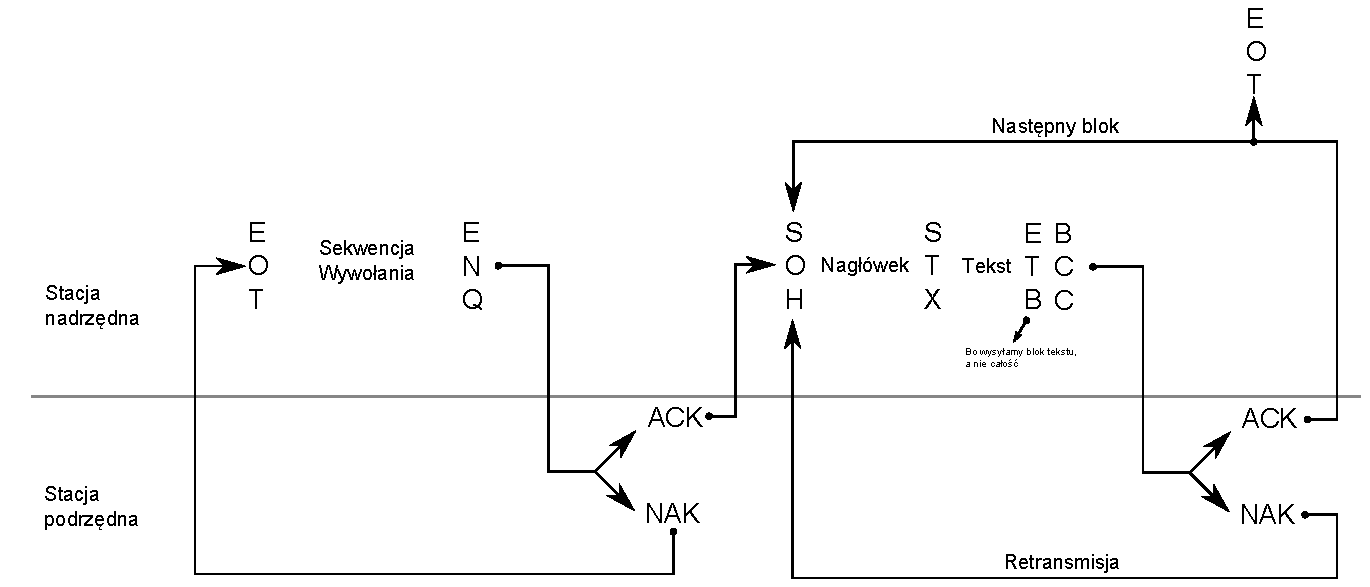
\includegraphics[width=12cm]{./images/image06.pdf} \\
			W sekwencji wywołania wybierany jest terminal, z którym zostanie nawiązane połączenie.
		\subsection{Nadania}
			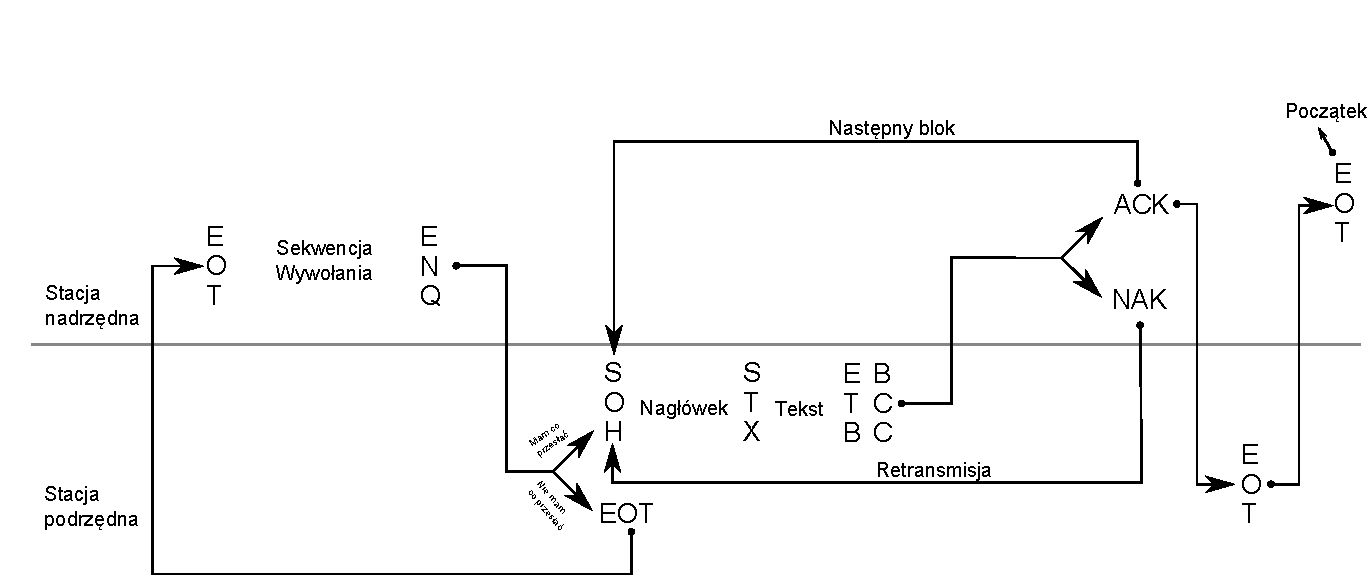
\includegraphics[width=12cm]{./images/image07.pdf}
		\subsection{Charakterystyka powyższych rozwiązań}
			\begin{itemize}
				\item SYN SYN dajemy gdy następuje zmiana kierunku transmisji (SOH, EOT, ACK, NAK)
				\item Mała kontrola poprawności. Tylko ramka (SOH ... BCC) jest jakoś chroniona. Pozostałe pakiety mogą zostać przekłamane i nadawca w żaden sposób nie dowie się czy odbiorca otrzymał dobre dane. Zatem dodajemy licznik czasu (timeout), dzięki któremu może wykryć błędy jak brak potwierdzenia odbioru.
			\end{itemize}
		\subsection{Z timeout}
			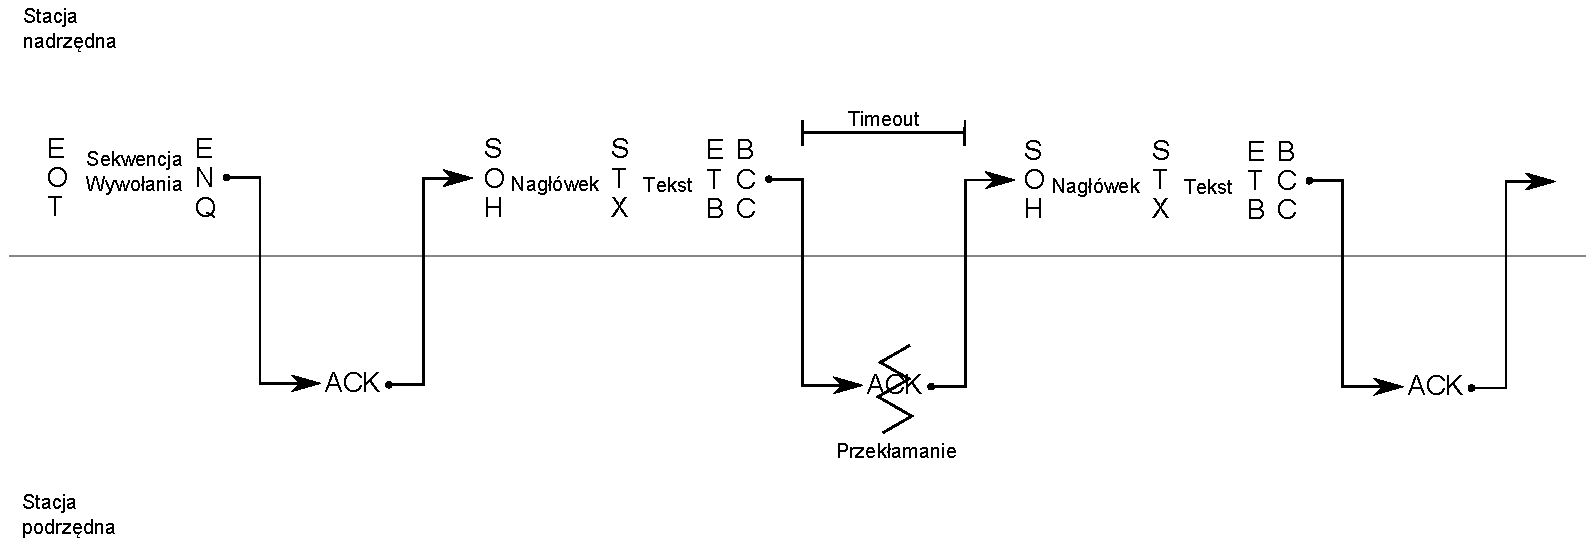
\includegraphics[width=14cm]{./images/image08.pdf}
			\subsubsection{Wada rozwiązania}
				Stacja podrzędna odbiera 2 bloki tekstu, w tym jeden zduplikowany, ponieważ nie została poinformowana przez timeout o przekłamaniu. Odbiorca nie jest w stanie stwierdzić, czy pakiet jest duplikatem czy nową informacją.
		\subsection{Numeracja potwierdzeń}
			Rozwiązanie problemu duplikatów: wprowadzenie numeru sekwencyjnego. 1-bit, zwiększający się zgodnie z arytmetyką modulo 2, umożliwia stwierdzenie czy pakiet jest wysyłany ponownie lub nie. Może być dodany do ACK lub NAK.\\
			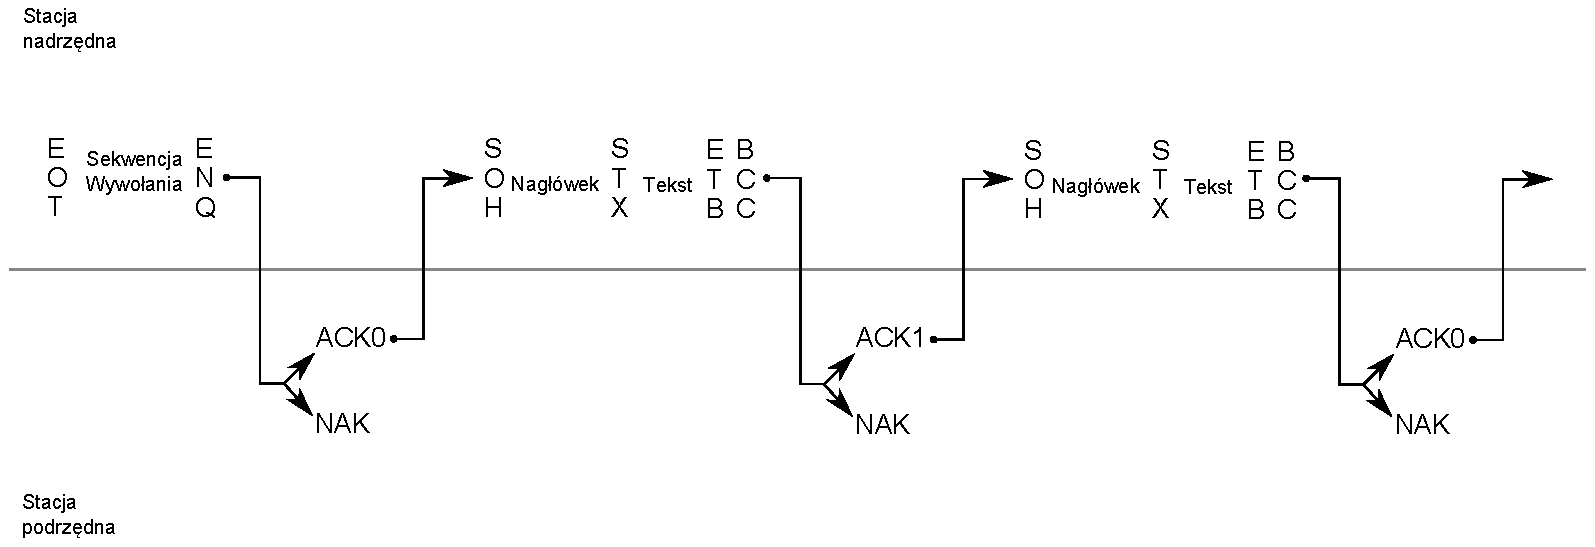
\includegraphics[width=14cm]{./images/image09.pdf}\\\\
			\subsubsection{Wada rozwiązania}
				Jeżeli stacja nadrzędna jest zajęta, to stacja podrzędna tego nie wie. To źle, bo stacja podrzędna zawsze wysyła jakiś sygnał (ACK / NAK).
		\subsection{Sterowanie przepływem}
			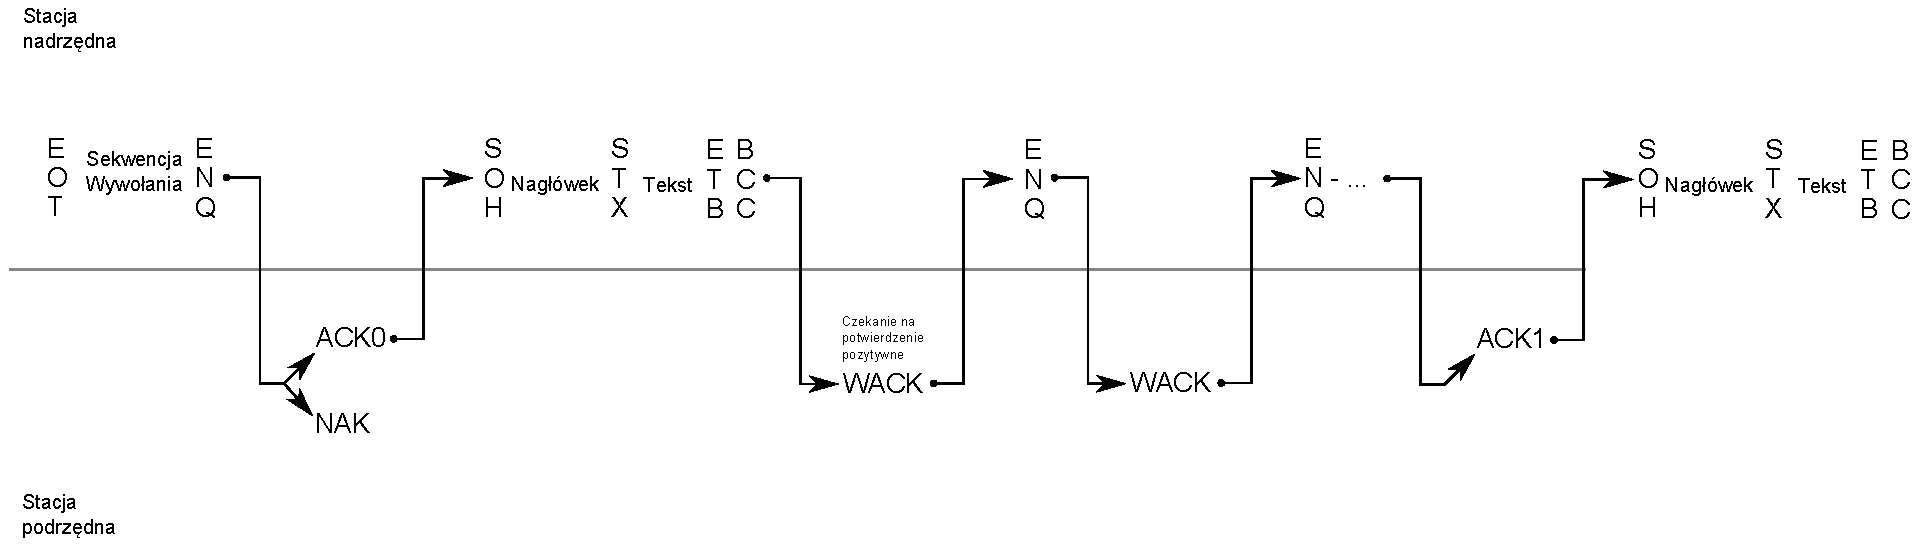
\includegraphics[width=14cm]{./images/image10.pdf}\\\\
			\textbf{WACK} - sygnał "czekaj na potwierdzenie". Używany gdy stacja podrzedna potrzebuje czasu na przetworzenie danych.
			\subsubsection{Wada rozwiązania}
				Wadą całego BSC jest brak możliwości korzystanie ze wszystkich znaków przy nagłówku i tekście, bo część z nich jest znakami kontrolnymi. Powstaje limit kombinacji bitów - brak przezroczystości. Skutkuje to tym, że nie można np. wysłać grafiki.
	\section{Przezroczysty blok w BSC}
		
\includegraphics[width=9cm]{./images/image11.pdf}\\
		Ten umożliwia przesyłanie grafiki.\\
		Jeśli w nagłówku lub tekście znajduje się znak DLE należy do powtórzyć.
	\section{Przebiegi czasowe}
		\begin{itemize}
			\item SN: sekwencja wywołania
			\item SP: Np. SYN SYN
			\item SN: Blok
			\item SP: 4B (SYN SYN DLE0) - czas marnowany
			\item SN: znów coś
		\end{itemize}


\part{Protokół o organizacji bitowej SDLC}
	Protokół SDLC ma za zadanie rozwiązać problem wydajnościowy związany z BSC. Protokół BSC, który zdefiniowaliśmy pod sam koniec, jest protokołem zatrzymania i czekania. Sprawia, że istnieje zagrożenie nieefektywnego wykorzystania łącza - nadawca może wysyłać znacznie mniej danych w jednostce czasu niż jest to możliwe (nawet tylko ułamek procenta).\\
	Rozwiązaniem jest zastosowanie mechanizmu \textbf{potokowego} - polega on na wysyłaniu wielu pakietów bez oczekiwania na potwierdzenie. Np. wysyłając 3 pakiety przed uzyskaniem potwierdzenia może przyspieszyć transfer 3-krotnie.\\
	Zastosowanie tego rozwiązania niesie ze sobą konsekwencje:
	\begin{itemize}
		\item Zwiększenie zakresu numerów sekwencyjnych (każdy musi mieć swój unikatowy numer, a wysyłamy ich więcej)
		\item Strona nadawcza i odbiorcza protokołu może być zmuszona do buforowania więcej niż jednego pakietu.
		\item Nowe metody usuwania błędów:
		\begin{itemize}
			\item Go-Back-N
			\item Powtarzanie selektywne
		\end{itemize}
	\end{itemize}
	\section{Łącze, ramki i flagi}
		\subsection{Format przesyłanych danych}
			\begin{itemize}
				\item \textbf{Łączem} przesyłamy ciągły strumień bitów, w nim są separatory.
				\item Separatory to niepowtarzalne kombinacje, które nazywamy \textbf{flagami}.
				\item Po fladze jest \textbf{ramka} i znów flaga. Można powiedzieć, że każda ramka jest otoczona dwiema flagami.
			\end{itemize}
		\subsection{Flaga}
			Flaga ma wartość $ 01111110 $ (inaczej 0x7E). Pojawia się problem gdy w pakiecie danych jest coś podobnego. Rozwiązanie: algorytm szpikowania zerami. Pomiędzy 5tą i 6tą jedynkę wstawia się techniczne zero ($ 011111\textbf{0}10 $). przy odbiorze drugiej flagi się je kasuje.
		\subsection{Format ramki}
			\begin{table}[h]
				\begin{tabular}{|c|c|c|c|c|c|}
					\hline
					FLAGA (1B)	&	Pole adresu (1B)	&	Pole sterujące (1B)	&	Dane	&	CRC (2B)	& FLAGA (1B)	\\ \hline
				\end{tabular}
			\end{table}
		\subsection{Adresowanie}
			Adres zawsze dotyczy terminala (odbiorcy lub nadawcy).\\
			ADR = 0xFF $ \longrightarrow $ transmisja rozgłoszeniowa.
			\subsubsection{Pole sterujące}
				\begin{itemize}
					\item Typ I (informacyjny)\\
					\begin{table}[h]
						\begin{tabular}{cccc}
							1                       & 3                         & 1                     & 3                         \\ \hline
							\multicolumn{1}{|c|}{0} & \multicolumn{1}{c|}{N(S)} & \multicolumn{1}{c|}{P/F} & \multicolumn{1}{c|}{N(R)} \\ \hline
						\end{tabular}
					\end{table}
					P/F - flaga sterują kierunkiem transmisji. Jeśli 1 to po zakończeniu odbioru następuje zmiana kierunku.
					\item Typ S (sterujący numerowany) \\
					\begin{table}[h]
						\begin{tabular}{cccc} \hline
							\multicolumn{1}{|c|}{1 0} & \multicolumn{1}{c|}{$ S_{1} S_{0} $} & \multicolumn{1}{c|}{P/F} & \multicolumn{1}{c|}{N(R)} \\ \hline
						\end{tabular}
					\end{table}
					\item Typ U (sterujący nienumerowany)\\
					\begin{table}[h]
						\begin{tabular}{cccc} \hline
							\multicolumn{1}{|c|}{1 1} & \multicolumn{1}{c|}{} & \multicolumn{1}{c|}{P/F} & \multicolumn{1}{c|}{} \\ \hline
						\end{tabular}
					\end{table}
					W pustych polach można przesłać polecenia sterujące. Typ wykorzystywany do zamykania i otwierania połączenia oraz do stanów awaryjnych.
					\item Pierwsza ramka z SN mówi według jakiego algorytmu będzie się odbywał przesył.\\
					\item Nowsze tryby przesyłu (z większymi licznikami):
					\begin{itemize}
						\item NRM - podobne do BSC, wykorzystany typ U. Tryb normalnej odpowiedzi.
						\item ARM - obie stacje niezależne, bez P/F. Równoległe asynchroniczne przesyłanie.
						\item ABM - przesył równoczesny, usunięcie stacji nadrzędnych.
						\item W przypadku użyciu wersji z 7-bitowym licznikiem istnieją jeszcze 3 tryby: SNRM, SARM, SABM (wszystkie z opcjonalnym E)
					\end{itemize}
				\end{itemize}
	\section{Adapter komunikacyjny}
		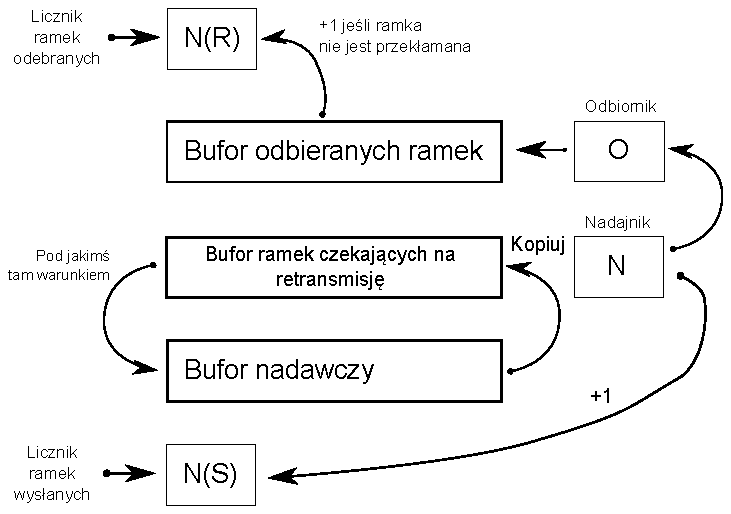
\includegraphics[width=10cm]{./images/image12.pdf}
	\section{Komendy sterujące}
		\begin{itemize}
			\item UA - nienumerowane potwierdzenie
			\item UI - nienumerowana informacja
			\item CMDR - odrzucenie polecenia (brak zgodny na dany typ, inaczej: Slave nie rozpoznaje komendy)
			\item FRMR - odrzucenie ramki niepasującej w ustalony schemat
			\item RD (\emph{remote disconnect}), DISC, DM (\emph{disconnect mode}) - zamykają połączenie
			\item XID
			\item Komendy numerowane
			\begin{itemize}
				\item RR N(R) - \emph{ready}
				\item RNR N(R) - \emph{not ready}
				\item REJ N(R) - \emph{rejection}\\
				Np. REJ, 1 - żądanie retransmisji ramek \textbf{od numeru 1}
				\item SREJ N(R) - \emph{selective rejection} - żądanie retransmisji wskazanej ramki. Break retransmisji grupowej.\\
				Np. SREJ, 1 - żądanie retransmisji \textbf{tylko} ramki nr 1.
			\end{itemize}
		\end{itemize}
	\section{Połączenia w SDLC}
		\subsection{Normalny tryb odpowiedzi}
			Wykorzystuje algorytm \textbf{Go-Back-N} - "cofnij się o N". Polega na prostej zasadzie: protokół może wysyłać wiele pakietów bez oczekiwania na potwierdzenie, jednak liczba niepotwierdzonych pakietów transferowanych w potoku nie może przekroczyć pewnej określonej liczby \emph{N}.\\
			Ilustracja problemu:\\
			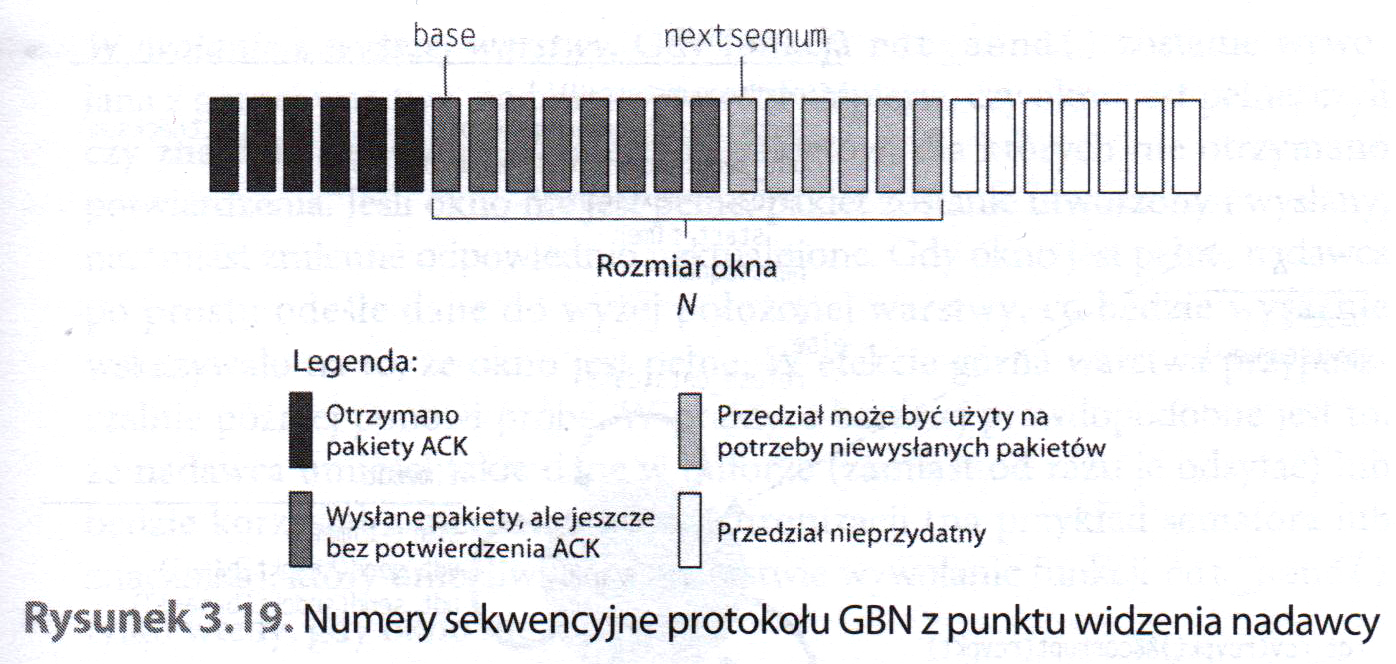
\includegraphics[width=10cm]{./images/image13.jpg}\\
			Zakres numerów sekwencyjnych dopuszczalnych w przypadku przesyłanych pakietów, dla których nie otrzymano potwierdzenia, wyróżniono jako \textbf{okno} o rozmiarze \emph{N}. W trakcie działania okno jest przesuwane wzdłuż zakresu numerów sekwencyjnych. Dlatego \emph{N} nazywamy \textit{rozmiarem okna}, a sam protokół GNB \textit{protokołem przesuwnego okna}.\\
			W protokole występują \textbf{zdarzenia}, które należy rozpoznać i obsłużyć:
			\begin{itemize}
				\item \textbf{Wywołanie z wyższej warstwy} - gdy z niej otrzymujemy pakiet, nadawca sprawdza czy okno jest pełne
				\begin{itemize}
					\item Jeśli nie, pakiet zostaje utworzony i wysłany, a zmienne odpowiednio uaktualnione.
					\item Jeśli tak, nadawca odsyła dane do warstwy wyższej, co oznacza zapełnienie okna, i wysyła dane później.
				\end{itemize}
				\item \textbf{Odebranie potwierdzenia ACK} - powiązane z pakietem posiadającym numer sekwencyjny \emph{n} zostanie uwzględnione w \textbf{potwierdzeniu skumulowanym}, które wskazuje, że wszystkie pakiety mające numery sekwencyjne aż do numeru \emph{n} włącznie zostały poprawnie przekazane odbiorcy.
				\item \textbf{Zdarzenie upłynięcia czasu} - związane z utraconymi lub znacznie opóźnionymi pakietami. Zegar jest używany w celu wyeliminowania utraconych pakietów lub tych, dla których nie otrzymano potwierdzenia. Jeśli upłynie określony czas, nadawca ponownie wyśle \emph{wszystkie} pakiety, dla których nie uzyskano potwierdzenia.
			\end{itemize}
			Przykład:\\
			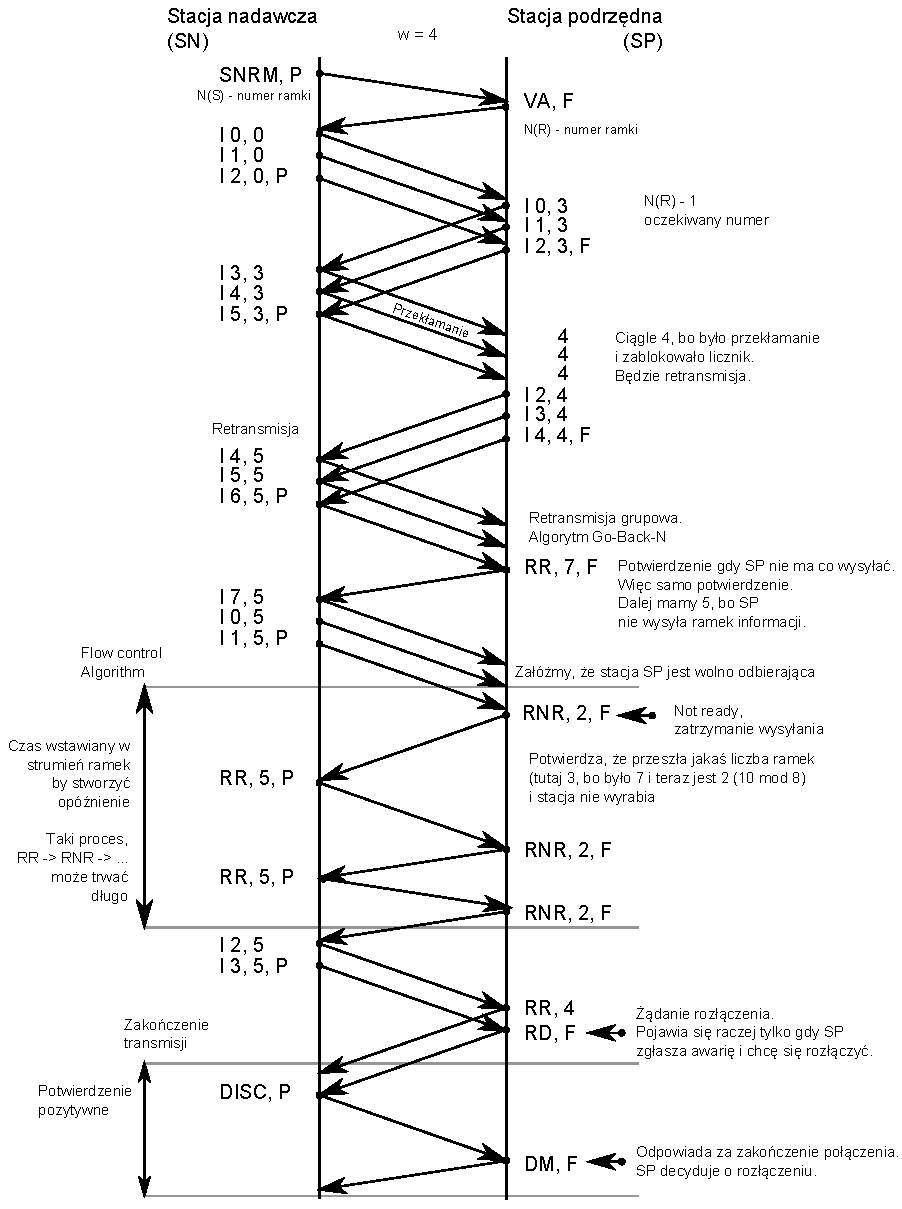
\includegraphics[width=14cm]{./images/image14.pdf}\\
			Optymalną wielkością okna jest 4. Stacja może wysłać tylko 4 ramki naraz, a potem musi czekać na potwierdzenie.
			\subsubsection{Timeout}
				Dotyczy każdej ramki\\
				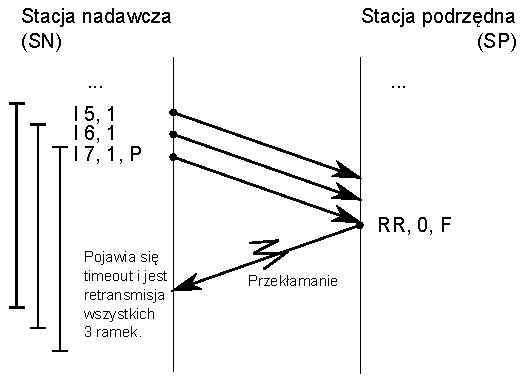
\includegraphics[width=6cm]{./images/image15.pdf}
			\subsubsection{Rodzaje potwierdzeń}
				\begin{itemize}
					\item Pozytywne
					\item Negatywne przez timeout
				\end{itemize}
		\subsection{Tryb asynchronicznej odpowiedzi (ARM)}
			SN i SP mogą wysyłać jednocześnie. Brak sztywnego przypisania na stację podrzędną i nadrzędną. RNR też tu działa.
			\subsubsection{Mechanizmy potwierdzenia}
				\begin{itemize}
					\item Pozytywne (stan NCR) - mówi, że nie trzeba się już zajmować którąś z ramek, która została potwierdzona.
					\item Negatywne (timeout) - wymusza retransmisję.
				\end{itemize}
			\subsubsection{Właściwości}
				\begin{itemize}
					\item Parametr \emph{w} pilnuje ilości przesyłanych ramek. Nadmiarowe muszą czekać i są przesyłane później.
					\item Sekwencja zakończenia podobna do poprzedniego trybu. Może być nawet RD, F, ale musi SP wysyłać potwierdzenia odebrania ramek od SN. Na końcu SN wysyła DISC.
					\item P i F są potrzebne tylko na początku.
					\item Timeout powinien być duży, ale nie za duży.
				\end{itemize}
				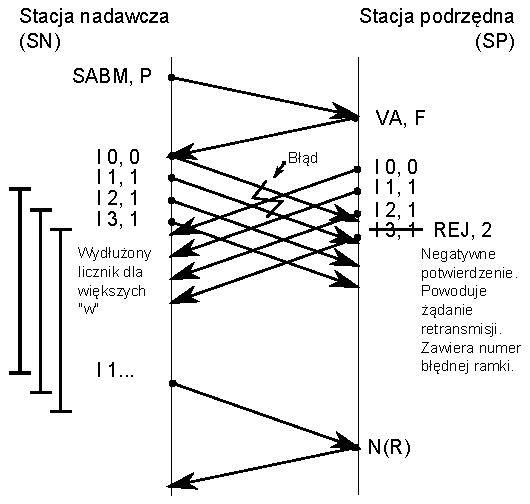
\includegraphics[width=6cm]{./images/image17.pdf}\\\\
				Wersja ze \textbf{SREJ} - retransmisja pojedynczej ramki\\
				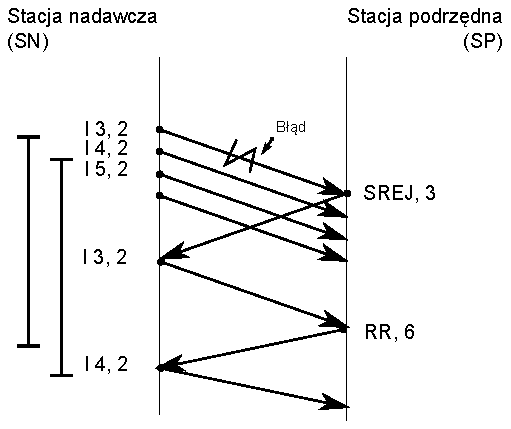
\includegraphics[width=6cm]{./images/image18.pdf}
			\subsubsection{Zrównoważony tryb działania (AMB (E) lub ABM - asynchronous balanced mode)}
				Dotyczy trybu asynchronicznego. E występuje dla dużych liczników.\\
				To samo, tylko stacja, która zaczyna nadawać zostaje oznaczona jako "SN".
		\subsection{Inne}
			SDLC jest zastrzeżony przez IBM, dlatego powstały rozwiązania alternatywne (HDLC)
	\section{Jakość łącza}
		Czyli wpływ kontroli błędów na łącze.\\
		\subsection{Bit Error Rate (BER)}
			BER $ ~ $ $ 10^{-4} $ \\
			Czasami zamiast tego liczy się FER - Frame Error Rate.
			\subsubsection{Przykład}
				Jest do przesłania 2 kB w blokach 256 B, $ w = 3 $\\
				\begin{equation}
				 N = \frac{2[kB]}{256[B]}=8 
				\end{equation}
				Oznacza to, że:
				\begin{itemize}
					\item 1 na 10 tysięcy bitów zostaje przekłamanych
					\item 1 na 1250 bajtów zostaje przekłamanych
					\item 1 ramka $ ~ $ 262 bajtów (6B nagłówka + 256B danych)
					\item $ \frac{1250}{262}=3,45 $ ramki
					\item Co 3.45 ramki jest przekłamane.
				\end{itemize}
				\textbf{Rozwiązanie}: więcej ramek przesyłanych (narzut organizacyjny protokołu).\\
				Wielkość ramek $ \searrow \rightarrow $ Narzut $ \searrow $ W $ \searrow \rightarrow $ Narzut $ \searrow $
		\subsection{Cechy}
			\begin{itemize}
				\item Stopa błędów 
				\begin{equation}
					q=\frac{ilosc\_bledow}{ilosc\_bitow\_transmitowanych} 
				\end{equation}
				\item Pole danych w SDLC wynosi 128B, ale może też być 64, 256, 1024
				\item Licząc stopę błędy bierzemy całą ramkę wraz z flagami, więc do tego 128 dodajemy 6 (134)
				\item Optymalna długość pola danych
				\begin{equation}
					D_{opt}=\frac{H+C\times{T_{out}}}{2}\times  [\sqrt{1-\frac{4}{(H+C\times{T})\ln{(1-q)}}}-1]
				\end{equation}
				Gdzie:
				\begin{itemize}
					\item H - długość nagłówka
					\item C - przepustowość łącza
				\end{itemize}
			\end{itemize}
		\subsection{Przykład}
			Dane:
			\begin{itemize}
				\item $ C=9600[bps] $ (bit na sekundę)
				\item $ T=50[ms] $ (timeout)
			\end{itemize}
			Dla:
			\begin{itemize}
				\item $ q=10^{-3} $, $ D_{opt}=715[b]=89[B] $
				\item $ q=10^{-4} $, $ D_{opt}=2262[b]=282[B] $
				\item $ q=10^{-5} $, $ D_{opt}=7155[b]=854[B] $
			\end{itemize}
			\textbf{Wniosek}: im mniejsza stopa błędu tym dłuższe optymalne pole danych.
	\section{Łącze radiowe}
		\begin{itemize}
			\item Dwa kanały: pierwszy z centrum komputerowego, drugi do CK.
			\item Problem dostępu do łącza: wbudowanie w terminal algorytmu dostępu do łącza:
		\end{itemize}
		\subsection{Algorytm dostępu do łącza}
			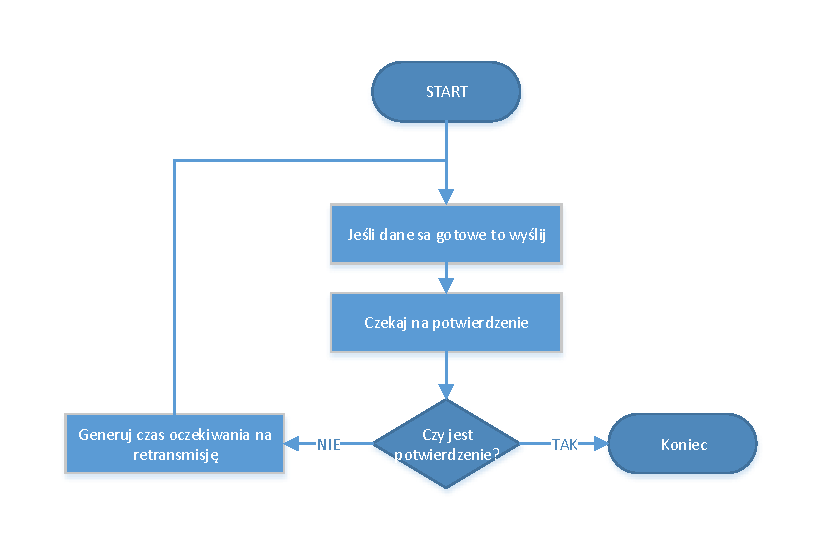
\includegraphics[width=10cm]{./images/image19.pdf}\\\\
			Retransmisja następuje z losowym opóźnieniem by ramki ponownie się na siebie nie nałożyły.\\
		\subsection{Protokół}
			Zastosowano protokół swobodnego dostępu, ALOHA.
	\section{Komunikacja kablowa}
		\subsection{Model}
			Jeden kabel, wiele stacji. Jak chce nadawać to nadaje, tylko czeka na potwierdzenie, jeśli nie nadejdzie, to dopiero retransmisja (algorytm swobodnego dostępu) (chyba). 
		\subsection{Algorytmy}
			\begin{itemize}
				\item CSMA (\emph{Carrier Sense Multiple Access}) - wykrywa występowanie zakłóceń, objawiają się w postaci dwóch ramek. Po wykryciu końca kolizji decyduje, która ramka czeka, a która jest retransmitowana.
				\item p-CSMA (\emph{persistent} CSMA)\\
				Punkt startu
				\item Algorytmy, które przerywają transmisję po wykryciu początku zakłócenia danej ramki
				\begin{itemize}
					\item CSMA / CD - wykrywanie kolizji, początek ETHERNETu
					\item CSMA / CA - zapobieganie kolizji, później, wcześniejsze zastosowanie w radiówce
					\item CSMA / CR - rozstrzyganie kolizji, lepszy wygrywa i kontynuuje przesył, słabszy musi znów wysłać
				\end{itemize}
			\end{itemize}
	\section{Dostęp do łącza}
		\subsection{Protokoły dostępu do łącza}
			\begin{itemize}
				\item Swobodnego dostępu (np. ALOHA)
				\item Częściowo kontrolowanego dostępu (np. CSMA / ...)
				\item Kontrolowanego dostępu - faza wykonania bez kolizji i faza gdzie może być.\\Sposoby kontroli:
				\begin{itemize}
					\item Planowanie transmisji
					\item Przekazywanie żetonu (token)
				\end{itemize}
			\end{itemize}
	\section{Częściowo kontrolowany dostęp (działanie CSMA / …)}
		\subsection{Algorytm dostępu}
			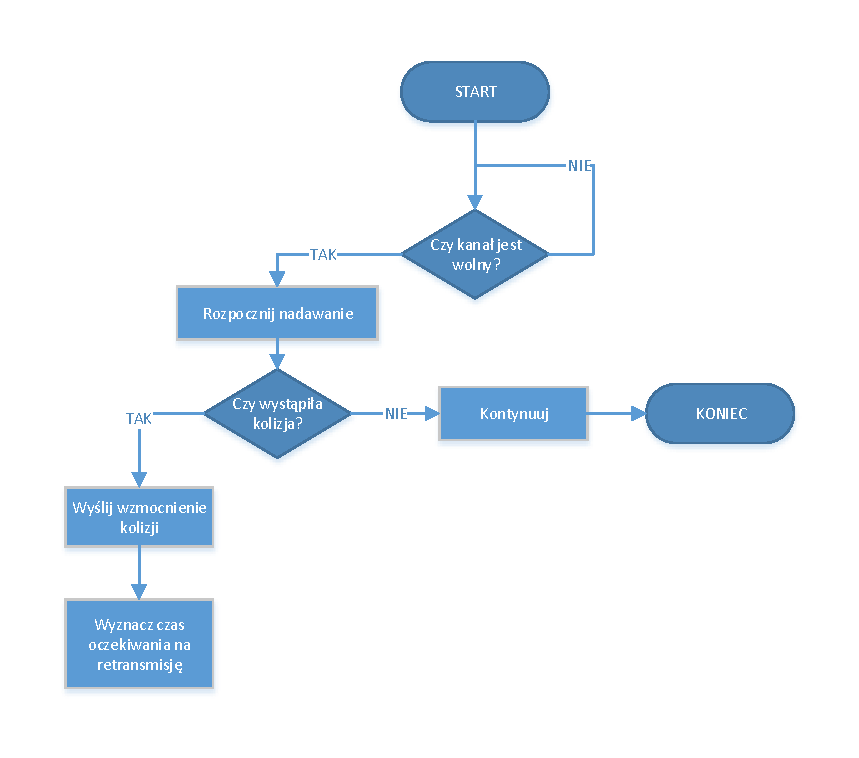
\includegraphics[width=10cm]{./images/image20.pdf}\\\\
			Algorytm oparty o kilka prostych zasad
			\begin{itemize}
				\item "nie przeszkadzaj" (sprawdza czy jest widoczna nośna) - zaczynamy nadawać gdy kanał się zwolni\\
				CSMA persistent, P(startu) = 1. Możliwe kolizje.\\
				CSMA p-persistent, P(startu) = p. (jakoś tak)
				\item "czy koliduje"?" (patrz wyżej)
			\end{itemize}
		\subsection{Czas do retransmisji}
			Oznaczany jako $ T_{R} $\\\\
			$ T_{R} = r(x)\times (2^{k}-1)\times T_{ob}$\\\\Gdzie:\\
			\begin{itemize}
				\item $ r(x) $ - liczba losowa z zakresu 0...1
				\item $ T_{ob} $ - czas obiegu łącza, w najgorszym wypadku podwojony czas propagacji
				\item $ k $ - liczba kolizji, czyli który raz się te ramki już zderzyły.
				\item Wraz ze zwiększaniem się liczby kolizji, możliwy zakres rośnie ekspotencjalnie. Jednak maksymalna wielkość $ k $ jest równa \textbf{10}. Dla $ k > 10 $ przyjmuje się $ k=10 $.
				\item Próbujemy szczęścia aż do $ k <=16 $, potem próby są przerywane.
			\end{itemize}
		\subsection{Cechy}
			Maksymalnie 2800 m do pokonania.\\
			Najgorszy czas 47,2 $ \mu s $.\\
			$ 51,2 \mu s=64B $ wyśle. W tym czasie mogą się zdarzyć kolizje.
		\subsection{Poprawna transmisja}
			Ramka musi być dłuższa niż 64B. Taki wymóg ma Ethernet.
			\subsubsection{Opcje}
				\begin{itemize}
					\item 3 segmenty i 2 repeatery
					\item 3 segmenty i 4 pół-repeatery
				\end{itemize}


\part{Sieć typu Ethernet}
	\section{Budowa}
		Standard Ethernet 2.0 wykorzystuje kabel koncentryczny.
		\subsection{Kabel koncentryczny}
			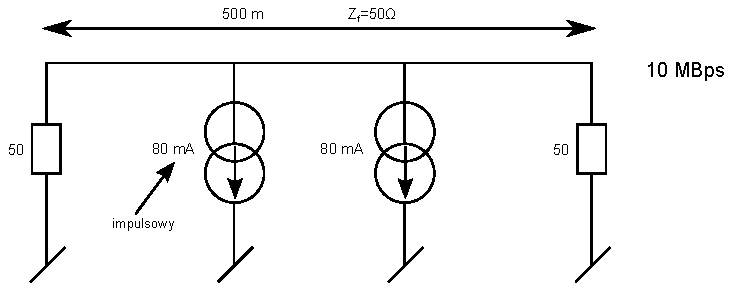
\includegraphics[width=10cm]{./images/image27.pdf}\\\\
			\textbf{Parametry}:
			\begin{itemize}
				\item $ U_{IC}=U_{p}\times e^{\alpha{l}} $
				\item $ \alpha{l} <= 6 dB|_{5 MHz} $
				\item $ \alpha{l} <= 8.5 dB|_{10 MHz} $
			\end{itemize}
		\subsection{Kodowanie}
			Standard wykorzystuje kodowanie Manchester.\\
			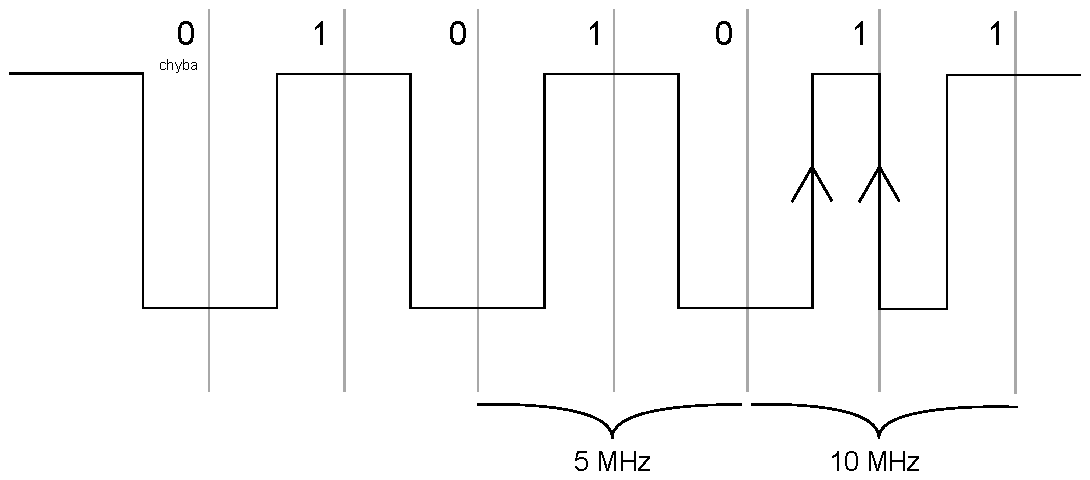
\includegraphics[width=7cm]{./images/image28.pdf}
		\subsection{Sprawdzanie kolizji}
			Chyba chodzi o zapobieganie kolizjom na poziomie sprzętowym.
			\begin{itemize}
				\item Sprawdzenie poziomu
				\item Pomiar wartości średniej prądu
				\item Wyłapywanie regularności szpilek
				\item $ T_{ob}=47.7 \mu{s} $
			\end{itemize}
			W trakcie transmisji początkowych 64 bajtów ramki może być złe.\\
			Mogą wystąpić 3 segmenty kolizji + $ 4 \frac{R}{2} $ + 2 segmenty łącza.
	\section{Ramka}
		To jest (chyba) ramka dla CSMA/CD.\\
		\begin{table}[h]
			\begin{tabular}{|c|c|c|}
				\hline
				\textbf{Element} & Wielkość & \textbf{Komentarz} \\ \hline
				\multicolumn{1}{|c|}{Preambuła} 	& 8 B & $ 7\times 10101010$, a na końcu $ 1010101\textbf{1} $. \\ \hline
				\multicolumn{1}{|c|}{Adres odbiorcy}	& 6 B &	MAC \\ \hline
				\multicolumn{1}{|c|}{Adres nadawcy}	& 6 B &	MAC \\ \hline
				\multicolumn{1}{|c|}{Kontrola}		& 2 B & 	\\ \hline
				\multicolumn{1}{|c|}{Pole danych}	& od 46 B do 1500 B	& \\ \hline
				\multicolumn{1}{|c|}{CRC}			& 4 B & \\ \hline
				Cisza na łączu między znakami		& 12 B & 9.6 $ \mu $s \\ \hline
			\end{tabular}
		\end{table}\\
		Każdy adres w Ethernecie powinien kończyć się zerem - adres stacji - jeden oznacza adres grupowy.
	\section{Zapobieganie kolizji}
		\subsection{Historyczne metody}
			\begin{itemize}
				\item Wprowadzenie Hubów - zmiana transmisji z szeregowej na równoległą.
				\item Switch: usuwa ramki kolizyjne. Zapamiętuje wysyłane ramki, które może bez końca retransmitować $ \rightarrow $ Znosi odpowiednie rozpiętości sieci $ \rightarrow $ wystarczy więcej switchy.
				\item Logiczny podział na małe sieci lokalne.
				\item Jumbo frame - pole danych do 9000 B. Wada: faworyzowanie pewnych stacji.
			\end{itemize}
		\subsection{Klasyczny algorytm}
			\subsubsection{Idea}
				Kilku chce wysłać, czekaj, retransmitują, znów problem.\\
				"Nie ma sensu czekać na wolne łącze, lepiej wygenerować pewien czas po którym ponownie sprawdzi się dostępność łącza".
			\subsubsection{Schemat blokowy}
				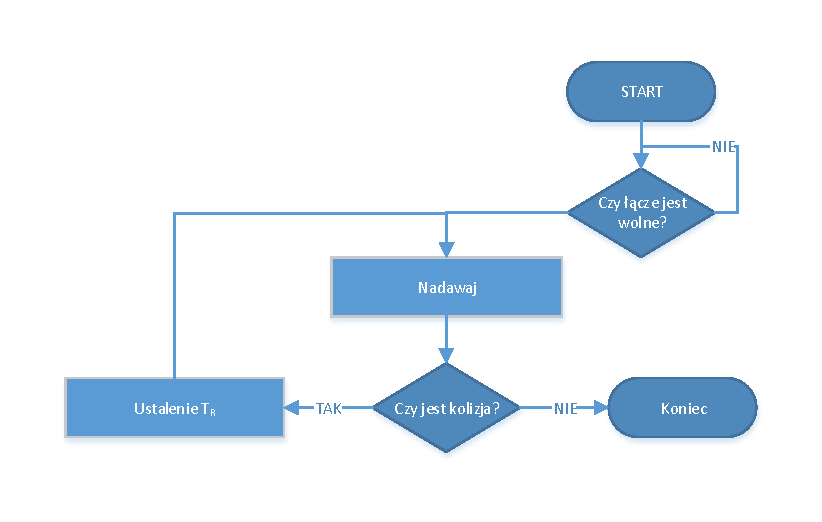
\includegraphics[width=10cm]{./images/image21.pdf}
		\subsection{CSMA/CA}
			Idea: unikanie kolizji\\
			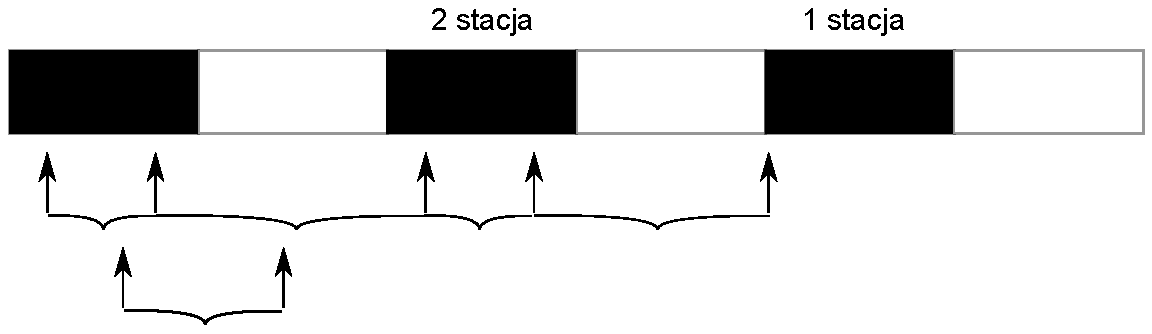
\includegraphics[width=10cm]{./images/image22.pdf}\\\\
			\textbf{Problem}: 1 stacja próbuje wysłać, 2 stacja próbuje wysłać.\\
			\textbf{Analiza}: jak widać brak kolizji. Najpierw patrzy czy łącze jest wolne, jeśli nie to generuje czas losowy, do następnej retransmisji. Czyli na początku ta generacja czasu, a nie na końcu jak w klasycznym Ethernecie.
		\subsubsection{Ramka}
			\begin{tabular}{|c|c|c|c|c|c|c|c|c|c|}
				\hline  & 2B & 2B & 6B & 6B & 6B & 2B & 6B & 0-23(?)B & 4B \\ 
				\hline Preambuła & Frame Control & Duration & A1 & A2 & A3 & Nr sekwencji (?) & A4 (opcjonalnie) & Dane & CRC \\ 
				\hline 
			\end{tabular}
		\subsubsection{Problem}
				Duże zakłócenia przy dużej ramce.\\
				FC i NS wspomagają fragmentację ramki.\\
				Wraca wzór Shannona z pestek:\\
				$$ C=B\times \log_2{(1+\frac{P_s}{P_w})} $$
		\subsubsection{Zmodyfikowane CSMA/CA}
			Wykorzystywane w radiówce.\\
			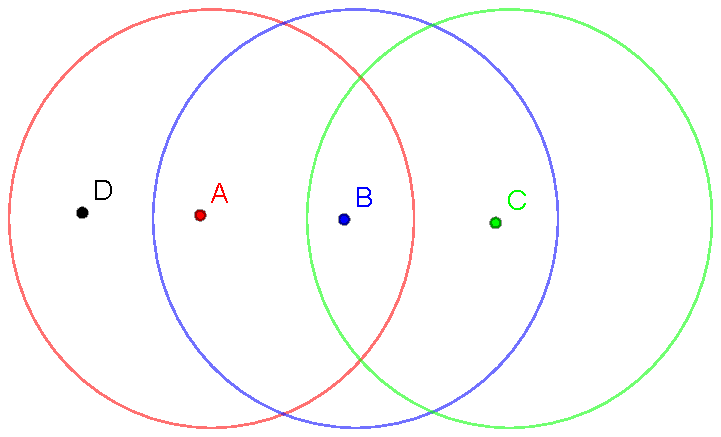
\includegraphics[width=10cm]{./images/image23.pdf}\\\\
			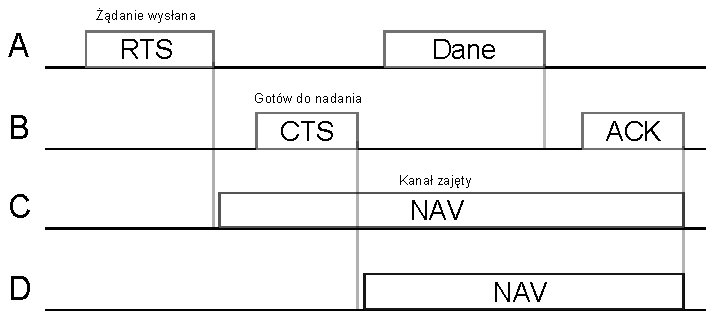
\includegraphics[width=12cm]{./images/image24.pdf}\\\\
			Czyli blokujemy pozostałe stacje (C i D), by nie zakłócały.\\
			Stację C blokuje stacja A, a stację D blokuje stacja B.\\
			Po stwierdzeniu, że kanał jest wolny, stacja musi poczekać jeszcze, bo może przyjść ACK.\\
			Jeśli stacja ustawi w ramce MORE to NAV (chanel busy flag) u innych stacji jest przedłużony o DURATION + ostatni ACK.
		\subsection{CSMA/CR}
			Umożliwia rozstrzyganie kolizji. Wykorzystywane w mikrosieciach (IIC (I$ ^2 $C)) (HiFi).\\
			Pierwsza część sygnału to pole adresu nadawcy. Najbardziej efektywny. Do sieci 1000 kB/s. S-7 m sieci.\\
			Sygnał nadawcy musi się rozejść po całej linii i wrócić, co zabiera ogromną ilość czasu.
		\subsection{Protokoły MAC (\emph{Media Access Control})}
			\begin{itemize}
				\item Swobodny dostęp (z potwierdzeniem)
				\item Algorytmy częściowo kontrolowanego dostępu CSMA (bez potwierdzenia)
				\item Algorytmy kontrolowanego dostępu (z potwierdzeniem / brak potwierdzenia dla transmisji danych)
				\begin{itemize}
					\item Rezerwacyjne
					\item Selekcyjne
					\item Jawnego wskazania (tzw. Token passing)
				\end{itemize}
			\end{itemize}
		\subsection{Algorytmy kontrolowanego dostępu}
			\begin{itemize}
				\item Algorytm z fazą planowania, gdzie jest dopuszczalne rozstrzyganie kolizji (z limitowaną kolizją).
				\item Algorytm z przekazywaniem uprawnienia, gdzie jest gwarantowany dostęp do łącza (przekazywanie żetonu (Token))
			\end{itemize}
			W tych algorytmach można wyróżnić dwie fazy:
			\begin{itemize}
				\item Planowania - widoczna dla wszystkich stacji, podzielona na szczeliny czasowe.
				\item Wykonania - superramka, uruchamia (...) szczelin czasowych
			\end{itemize}
		\subsection{Algorytmy z fazą planowania}
			Dopuszczalne rozstrzyganie kolizji (z limitowaną kolizją).
			\subsubsection{Algorytm rezerwacyjny}
				Rezerwacja prawa nadawania. Dzieli się na dwie fazy:
				\begin{enumerate}
					\item Rezerwację (faza planowania)
					\item Wykonanie (faza wykonania)
				\end{enumerate}
				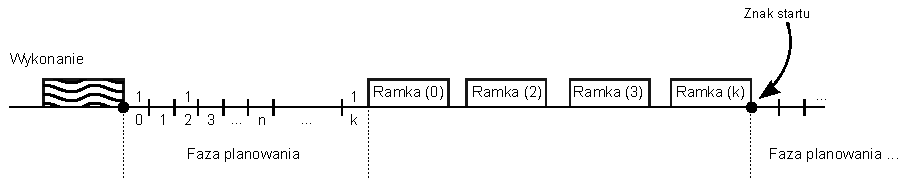
\includegraphics[width=11cm]{./images/image25.pdf}\\
				\textbf{Faza planowania} - to są szczeliny czasowe.
				\begin{itemize}
					\item Każda stacja ma przypisanie do jednej z nich.
					\item Jeśli stacja chce transmitować to wstawia 1 w swojej szczelinie czasowej.
					\item Jeśli nie potrzebuje dostępu, to nie.
					\item Po 1 bit na każdą szczelinę czasową.
				\end{itemize}
				Zwykle grupuje się stacje i każda grupa otrzymuje po jednej szczelinie czasowej (wówczas liczba szczelin $ < $ liczba stacji).\\
				Zawsze musi być minimum jedna ramka, bo musi być widoczny koniec transmisji.\\
				\textbf{Działanie}: wysyłamy adres stacji z grupy, ale są kolizje. Tu włącza się metoda generacji czasu na retransmisję itp. Jeśli nie zdąży wysłać, bo już zacznie wysyłać, to czeka na ponowne pojawienie się szczelin czasowych.\\
				W fazie planowania mogą wystąpić kolizje, ale dla każdej szczeliny kolizje są rozdzielane.\\
				Wykorzystywany w sieciach o dynamicznych priorytetach.
			\subsubsection{Algorytm selekcyjny}
				Selekcja wstępna, czyli która stacja ma prawo nadawania. Dzieli się na dwie fazy:
				\begin{enumerate}
					\item Selekcję (faza planowania) - - tu rozstrzyga się, która ramka przypadnie na którą stację.
					\item Wykonanie (faza wykonania)
				\end{enumerate}
				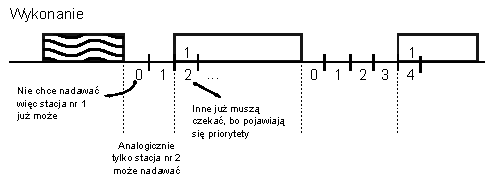
\includegraphics[width=10cm]{./images/image26.pdf}\\
				Powyższy rysunek przedstawia malenie priorytetu.\\
				Na jedną szczelinę może przypaść więcej niż jedna stacja (grupowanie).\\
				WAŻNE: stacje, które muszą być wykonane są wysyłane jako pierwsze i do tego pojedynczo, a nie w grupie (jedna na jedną szczelinę). Mimo to, zwykle wykonuje się w grupach.
				\begin{itemize}
					\item  Jeśli w trakcie nadawania superramki w sieci pojawi się nowa stacja, to musi ona poczekać do końca transmisji (początku kolejnej superramki), aby być uwzględniana w algorytmie.
					\item Problem pojawia się, gdy z sieci zniknie stacja w trakcie nadawania - nie wiadomo, kiedy znów nadejdzie daza planowania, a możliwe że na nieobecną maszynę przypadnie akurat jakaś ramka.
					\item Zazwyczaj stosuje się algorytmy hybrydowe, aby uniknąć takich sytuacji.
				\end{itemize}
		\subsection{Algorytmy z przekazywaniem uprawnień (Token)}
			\subsubsection{Co to jest Token?}
				Token to specjalna ramka sterująca.\\
				Token bus jest zdefiniowany w IEEE.802.4.
			\subsubsection{Idea działania}
				Stacja przechowuje adres poprzednika i następcy. Powstaje wówczas lista adresów stacji:\\
				$ A_1 \rightarrow A_2 \rightarrow A_3 \rightarrow ... \rightarrow A_n \rightarrow ... \rightarrow A_k \rightarrow A_1 $ ...\\
				Ilustracja przekazywania tokenu.\\
				Parametry:
				\begin{itemize}
					\item Czas korzystania z tokenu: $ T_k~40kbit $
					\item No Token Timer: $ T_{NTokT}=n\times T_k $, gdzie $ n $ to liczba stacji (?)
				\end{itemize}
			\subsubsection{Wada}
				Wszystko się sypie gdy zostaje przekłamany Token. Stacja czeka, orientuje się, że sieć się sypła, a następnie stacje walczą o to, która stworzy nowy Token.
				\begin{itemize}
					\item Algorytm "głosowania Tokenu", w końcu któraś wygra.
					\item Algorytm włączania stacji do listy, czyli zgłaszanie następcy (ponowna walka).
					\item Problem opuszczania sieci.
				\end{itemize}
			\subsection{Sieć pierścieniowa (Token Ring)}
				Zdefiniowana w IEEE 802.4 (?)
				Zastosowanie innej (pierścieniowej) topologii sieci. Eliminuje ona wcześniejsze problemy.\\
				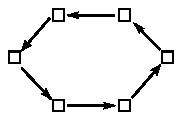
\includegraphics[width=7cm]{./images/image29.pdf}
				\begin{itemize}
					\item Transmisja tylko w jednym kierunku. Dzięki temu sieć może mieć wiele kilometrów.
					\item Stacje nie wiedzą co się dzieje u innych.
					\item Ciężko w niej znaleźć miejsce przerwania.
				\end{itemize}
				Sieć dwupierścieniowa (Token Ring).\\
				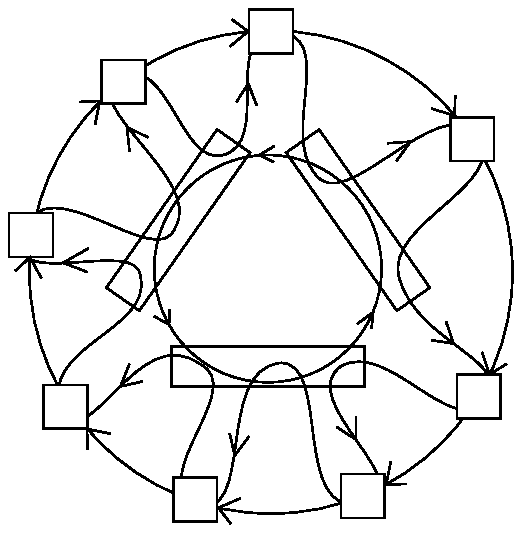
\includegraphics[width=7cm]{./images/image30.pdf}\\
				Dwa pierścienie: jeden zewnętrzny, drugi wewnętrzny (rezerwowy). Jeśli jeden przesyła w lewo, to drugi w prawo. Jeżeli zewnętrzny zostanie przerwany, to wewnętrzny zajmuje się załataniem tego.\\
				\textbf{Wada}: jeżeli w sieci nie ma Tokenu to występują kolizje.
			\subsection{Kodowanie informacji}
				Kodowanie dla sieci opartych o Token.\\
				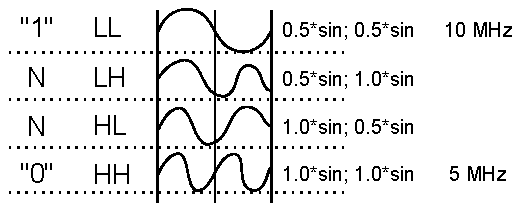
\includegraphics[width=7cm]{./images/image31.pdf}\\
			\subsection{Ramka}
				\begin{table}[h]
					\begin{tabular}{|c|c|c|c|c|c|c|c|cc}
						\hline
						N & N & 0 & N & N & 0 & 0 & 0 & SD & start ramki \\ \hline
						N & N & 1 & N & N & 1 & 1 & 1 & ED & koniec ramki \\ \hline
					\end{tabular}
				\end{table}
				Te "N" mówią, że to SD lub ED, a nie zwykłe dane. Więc tu nie używamy metody szpikowania zerami i tym podobnych.
				\subsubsection{Token Bus}
					\begin{table}[h]
						\begin{tabular}{|c|c|c|c|c|c|c|}
							\hline
							SD & FC & DA & SA & Dane & CRC & ED \\ \hline
						\end{tabular}
					\end{table}
					Gdzie:
					\begin{itemize}
						\item SD - Start Delimiter, ma postać NN0NN000, 1B
						\item FC - Frame Control (czasami zwany też Flow Control), czy to transmisja w jednym kierunku czy np. żądanie przesyłu odpowiedzi. Przekazuje informacje sterujące. 1B
						\item DA - Destination Address (6B / 2B)
						\item SA - Source Address (6B / 2B)
						\item ED - End Delimiter, ma postać NN1NN111, 1B
					\end{itemize}
				\subsubsection{Token Ring}
					\begin{table}[h]
						\begin{tabular}{|c|c|c|c|c|c|c|c|c|}
							\hline
							SD & FC & FC & DA & SA & Dane & CRC & ED & FS \\ \hline
						\end{tabular}
					\end{table}
					Gdzie:
					\begin{itemize}
						\item AC - adres rozpoznany, 1 - ok, 0 - nie (ramka skopiowana (jakoś tak)). Służy do przekazywania informacji sterujących jak np. wybranie pierwotnego posiadacza tokenu.
						\item FS - Frame Status
					\end{itemize}
			\subsection{Budowa bajtu FC}
				\subsubsection{Budowa}
					\begin{tabular}{|c|c|c|}
						\hline Rodzaj ramki (2b) & Przeznaczenie ramki (3b) & PPP (3b) \\ 
						\hline 
					\end{tabular} 
				\subsubsection{Rodzaje ramki}
					\begin{itemize}
						\item 00 - ramka kontrolna
						\item 01 - ramka  z danymi
						\item 10 - ramka konfiguracyjna (station management, do ustalania budowy sieci)
					\end{itemize}
				\subsubsection{Przeznaczenie ramki}
					\begin{itemize}
						\item 000 - żądanie (command), brak odpowiedzi
						\item 001 - żądanie i odpowiedź
						\item 010 - odpowiedź
					\end{itemize}
				\subsubsection{Bity PPP}
					\begin{itemize}
						\item Dla ramki z danymi oznaczają one priorytet
						\item Dla ramek kontrolnych definiuje się tutaj rodzaj ramki. 
					\end{itemize}
			\subsection{Problemy związane z Tokenami (wadliwe stany)}
			\begin{itemize}
				\item Brak Tokenu (najczęściej pojawia się przy samym starcie sieci) 
				\item Więcej niż jeden Token
				\item Zabezpieczenie przy przekazywaniu tokenu (należy się upewnić, czy token został dobrze przekazany)
				\item Nagłe zniknięcie Tokenu - zdarza się, gdy stacja aktualnie przetrzymująca Token opuszcza sieć
				\item Nowa stacja w sieci (zmiany w liście stacji)
			\end{itemize}
			\subsection{Timery (dostęp do łącza)}
				\subsubsection{Parametry}
					\begin{itemize}
						\item \textbf{THT} (\emph{Token Hold Timer}) - maksymalny czas przetrzymania Tokenu, równy \emph{n} bitów
						\item \textbf{NTT} (\emph{Not Token Timer}) - czas czekania na token. $ NTT=N\times THT $, gdzie \emph{N} to liczba stacji. Gdy trwa za długo to sieć pada.
						\item Problem pojawia się gdy przejdzie cały timer, a tokenu brak.
						\item Trzeba utworzyć listę adresów log (...). Każda stacja musi pamiętać dwa adresy: poprzednika i następnika.
					\end{itemize}
			\subsection{Algorytm rozstrzygania kolizji}
				Dla Token Bus: stacja, która chce coś wysłać, w ramce w FC wysyła CT - zgłoszenie tokenu. Potem stacja walczy z innymi.
				\begin{itemize}
					\item W sieci pierścieniowej stacje robią opóźnienie 1 bit.
					\item Stacje walczą o dostęp wg algorytmu rywalizacji. Jeśli adres nadawcy jest niższy niż mój, to ja wysyłam własną. Jeśli jego wyższy to retransmisja (jego ramkę dalej ?).
					\item Po przejściu całej sieci ramka ma adres zwycięzcy. Przez to opóźnienia. Wtedy ramka dodatkowa, która mówi, że jest już zwycięska i trzeba już normalnie przesyłać.
					\item W pierścieniowej technologii są potwierdzenia. Na końcu ramki dokleja się informację czy ramka była poprawnie wysłana i odebrana oraz czy zrobiono kopię tej ramki (ta odbierająca robi kopię). Na A lub C musi być jeden, że ok, lub zero, jeśli nie ok. Jeśli A i C = 1, to wszystko ok.
					\item Czyszczenie sieci pierścieniowej: nadawca coś wysyła, a jeśli coś do niej wchodzi w trakcie to są to śmieci, więc je usuwa. Usuwa też swoją ramkę po przejściu przez sieć.
				\end{itemize}
			\subsection{Cambridge Ring}
				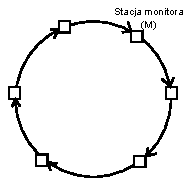
\includegraphics[width=4cm]{./images/image32.pdf}\\
				Pojemność informacyjna pierścienia $ 20\mu{s} $ gdy $ 4km $ sieci / 200 bit.\\
				Każda stacja M generuje miniramki o długości 40 bit.\\
				\begin{itemize}
					\item Liczba bitów w pierścieniu $ N_{ring}=\frac{L}{\frac{2}{3}C}\times \frac{1}{V}$, gdzie: \emph{L} to długość kabla łącza; \emph{V} to szybkość nadawania.
					\item Liczba bitów pamiętanych na kablach $ n=\frac{T_p}{T_b} $
					\item $ N_{ramek}=N_{ring}+N_{stacji}=\sfrac{4N}{40bit}$
				\end{itemize}
				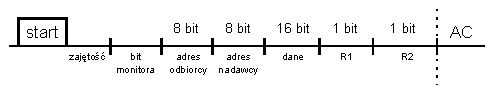
\includegraphics[width=7cm]{./images/image33.pdf}
				\begin{itemize}
					\item Sieć CR wykorzystuje monitor - wydzieloną stację.\\
					Monitor generuje "strumień" miniramek. Z = 1, czyli ktoś zajął tę ramkę i wpisał do niej dane (czyli używa się tej ramki do przesyłu).\\
					M = 1, czyli monitor już tę ramkę widział. Monitor skasuje tę ramkę gdy odczyta ją i ta ramka ma n = 1. Za drugim razem ??\\
					Gdy trzy pierwsze bity (startu, zajętości i monitora) są równe 1 to oznacza, że ramka obiegła cały pierścień i monitor wysyła nową tackę (??) informacyjną.
					\item Szybkość transmisji: $ \frac{2B}{T_{ob}} $, gdzie $ T_{ob} $ to czas obiegu, który trwa 30 $ \mu s $.
					\item Najgorsze rozwiązanie pod kątem serwisowania.
				\end{itemize}
				\subsubsection{Algorytm włączania rejestru}
					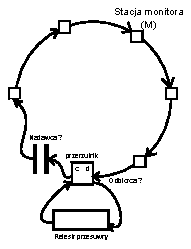
\includegraphics[width=7cm]{./images/image34.pdf}\\
					Dzięki temu może przesyłać duże ramki. Część wchodzi do rejestru przesuwnego.
				\subsubsection{Protokół drzewa rozpinanego}
					\emph{Spanning Tree Protocol}. Przydatne przy sieci pierścieniowej z repeaterem, która posiada wiele podstacji. Jeśli występuje retransmisja to trwa ona w kółko dzięki zamkniętemu obiegowi.


\part{Projektowanie topologii sieci}
	Kolejnym problemem w komunikacji jest ograniczenie zasięgu sieci przez długość kabli lub zasięg transmisji. Potrzeba więc wykorzystać pośredników.\\
	\textbf{Przykładowe rozwiązania}:
	\begin{itemize}
		\item Proste: połączenie każdego z każdym, ale nie jest to efektywna metoda.
		\item Lepsze: każdy z elementów posiada minimum 2 połączenia - w razie awarii jednej ze stacji ma alternatywę.
	\end{itemize}
	W projektowaniem topologii związanych jest kilka istotnych zagadnień.
	\section{Uzgodnienie gotowości udziału w transmisji}
		\subsection{Tryb połączeniowy}
			\subsubsection{Idea rozwiązania}
				Stacja A wysyła żądanie wyznaczenia trasy do stacji Z. Nazywamy to jako "pakiet żądania wykonania połączenia". Pakiet trafia do stacji B i jeśli ona może wysłać go dalej to odsyła potwierdzenie i szuka dalszej drogi. Fakt przesłania żądania zestawienia połączenia jest odnotowywany w każdym węźle przez który ten pakiet przechodzi (ID połączenia).\\
				W końcu ten trafia do stacji Z i jeśli stacja Z się zgadza na połączenia to odsyła pakiet odpowiedzi pewną drogą (która wcale nie musi być zgodna z tą, którą przyszło żądanie) do stacji A. Dzięki temu, że w węzłach istnieją ID połączeń mamy wyznaczoną ścieżkę przez którą będą przebiegać komunikaty z A do Z, a nawet dwie.
			\subsubsection{Pakiet}
				\begin{tabular}{|c|c|}
					\hline ID połączenia & reszta \\
					\hline 
				\end{tabular}
			\subsubsection{Cechy trybu}
				W tym trybie nie ma problemu dublowania pakietów. Natomiast jeżeli jedno połączenie wysiądzie (np. na wskutek awarii stacji) to pojawia się poważny problem.
		\subsection{Tryb bezpołączeniowy}
			\subsubsection{Idea rozwiązania}
				Pakiet danych wysyłany wprost do sieci, niezależny przesył.
			\subsubsection{Pakiet}
				\begin{tabular}{|c|c|c|}
					\hline Adres odbiorcy & Adres nadawcy & reszta \\ 
					\hline 
				\end{tabular}
			\subsubsection{Cechy trybu}
				Tu mogą się zdarzyć duplikaty ramek itp. ale gdy któryś węzeł padnie to jest szansa, że wszystko dalej będzie działać.\\
				W tym trybie działa większość sieci, w tym sam wielki Internet.
	\section{Tryb pracy sieci}
		\subsection{Komutacja kanałów (\emph{channel switching})}
			Rezerwacja kanałów od Nadawcy do Odbiorcy. Na czas połączenia wszystkie połączenia od nadawcy do odbiorcy, włącznie z połączeniami pośrednimi, sa zestawione i zablokowane. Jest związany z trybem połączeniowym.
		\subsection{Komutacja informacji (\emph{information switching})}
			Zamiast rezerwacji z góry wszystkich kanałów potrzebnych do komunikacji (komutacja kanałów) wyłącznie część między stacjami jest rezerwowana. Informacja jest przekazywana z węzła do węzła.
			\subsubsection{Przykład}
				Wysyłamy ze stacji A do C przez B. Ze stacji A przesyłamy wiadomość do B i tylko ten fragment kanału jest zajęty. Stacja B potwierdza odbiór i teraz ona zajmuje się znalezieniem C - połączenie pomiędzy stacjami A i B jest wolne. Tu komunikat musi być zapamiętany przez stację pośrednią. Jest to komunikacja typu \textbf{\emph{store \& forward}}
			\subsubsection{Problem}
				Wielkość informacji - każda stacja musi ją zapamiętywać.\\
				Rozwiązania:
				\begin{itemize}
					\item \textbf{Komutacja wiadomości} (\emph{information switching}): zapis całości informacji w buforach w buforach itp. (chyba), limit 8kB, technologia ARPANET
					\item \textbf{Komutacja pakietów} (\emph{packet switching}): dzielenie informacji na pakiety o stałym rozmiarze.
				\end{itemize}
	\section{Adresacja}
		Wykorzystywana jest adresacja \textbf{IP}.
	\section{Wybór drogi (\emph{routing})}
		\subsection{Diagram rozwiązań}
			Najpierw był routing źródłowy (\emph{source routing}), czyli ręczne wyznaczanie drogi przez nadawcę. Następnie pojawiły się rozwiązania w postaci algorytmów.\\\\
			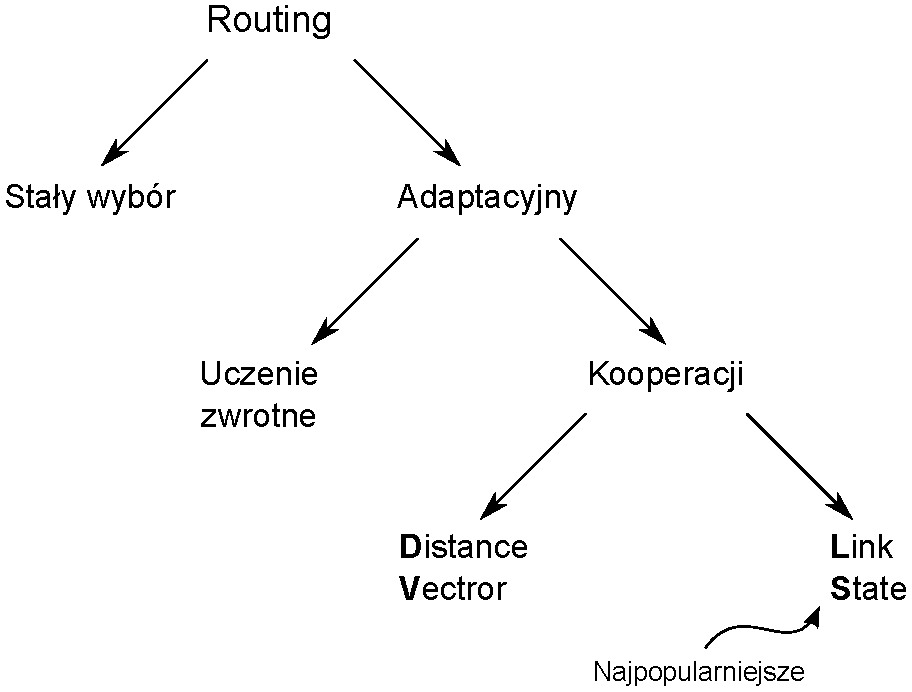
\includegraphics[width=8cm]{./images/image35.pdf}
		\subsection{Nomenklatura}
			\begin{itemize}
				\item Dużymi literami oznaczamy węzły
				\item Małymi literami oznaczamy ścieżki
			\end{itemize}
		\subsection{Algorytmy stałego wyboru}
			Algorytm statyczny, drogę wyznacza administrator na sztywno.
		\subsection{Algorytmy adaptacyjne}
			Algorytm dynamiczny, każdy węzeł zbiera informacji potrzebne do wyznaczenia trasy. Decyzja jest podejmowana na podstawie informacji uzyskanych na podstawie przesłanych wcześniej pakietów. Każdy węzeł wyznacza z osobna gdzie iść dalej.\\
			Z tym typem algorytmów związane sa następujące zagadnienia:
			\subsubsection{Zdobywanie informacji}
				\begin{itemize}
					\item \textbf{Uczenie zwrotne} - dodanie dodatkowego pola, gdzie przechowywane sa informacje jak np. znacznik czasu (timestamp) wysłania pakietu. Dzięki temu węzeł wie jak długo szedł pakiet. następnie robi tabelkę. Np.\\
					\begin{tabular}{|c|c|c|c|c|}
						\hline  &  & Zi &  &  \\
						\hline  &  & B & C & K \\ 
						\hline Interfejs & et1 & $ t_{Be1} $ &  &  \\ 
						\hline  & et2 & $ t_{Be2} $  & & \\ 
						\hline  & et3 & $ \inf $ &  &  \\ 
						\hline 
					\end{tabular}\\
					Na początku tablica jest pusta, co jest problemem. należy utworzyć początkową tablicę w jakiś sposób np. algorytmem stałego wyboru. Jeżeli przyjąć, że każdy timestamp jest równy, to wtedy jako jako informację można przechowywać liczbę węzłów, przez którą się przechodzi (jednak prawie zawsze timestampy są różne). \\
					Problem: konieczne są uaktualnienia tabelki. Jeżeli zabraknie update'u, wartość jest zatępywana przez nieskończoność (w praktyce: nie przesyłaj pakietów tą ścieżką). Początkowo tabela jest wypełniana samym nieskończonościami, dlatego wraz ze startem należy użyć wartości wyliczonych przez inny algorytm (potem uczenie zwrotne staje się samowystarczalne).
					\item \textbf{Algorytm kooperacji (samodzielnego badania (?))} - każdy węzeł odpytuje otoczenie, jakie węzły sa obok niego, wysyła żądanie echa i otrzymuje odpowiedzi. Dzięki temu zna również czas. Echo musi czekać na obsługę jak każdy inny pakiet. Dzięki temu przesyłaniu (echa itd.) wychodzi metryka łącza.\\
					Tutaj informacja ma swój czas życia (30 - 60 $ \mu s $). Jeżeli żaden pakiet nie przechodzi ta drogą to znaczy, że coś jest z nią nie tak.\\
					Rodzaje:
					\begin{itemize}
						\item \textbf{\emph{distance vector}} - wysyła pełną tablice routingu do sąsiadów (drogi dostępne w otoczeniu i metryki)
						\item \textbf{\emph{link state}} - przesyła do wszystkich węzłów informacje, że istnieje takie a takie łącze i metryka (koszt) tego łącza. Na podstawie tego, "wizualizowany" jest graf połączeń.
					\end{itemize}
				\end{itemize}
		\subsection{Inne algorytmy}
			\begin{itemize}
				\item Zalewania (transmisji \emph{broadcast}) - wysyłanie wszędzie w TTL. Bardzo nieoptymalny, ale zawsze działa (w końcu dotrze...). Pozwala ogarnąć nawet najbardziej zdezinformowaną sieć.
				\item Gorącego ziemniaka - wyślij do najbliższego / najlepszego z TTL (najmniej obciążonego) sąsiada. Problem: może stworzyć nieskończoną pętlę.
			\end{itemize}
		\subsection{Wyznaczanie tablicy routingu}
			Przykładowa sieć.\\
			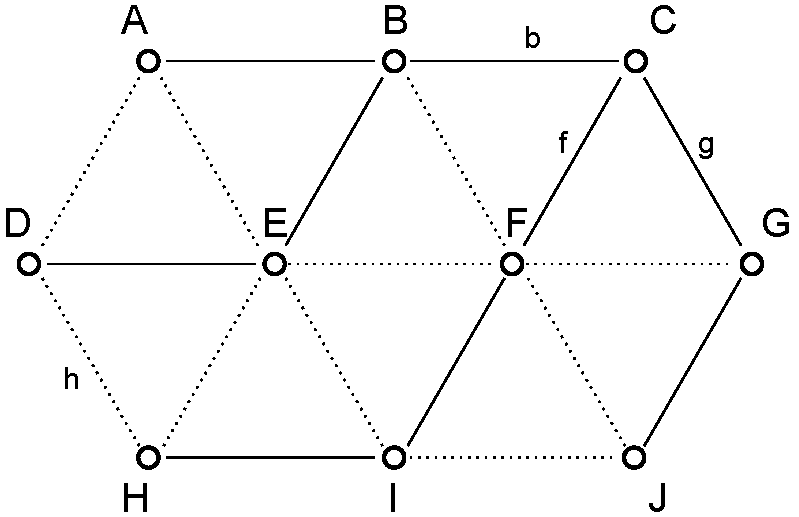
\includegraphics[width=7.5cm]{./images/image38.pdf}\\
			Linie przerywane oznaczają brak drogi z jednej stacji do drugiej.
			\subsubsection{Graf drzewa spływu}
				Wyciąć te które mogą powodować zapętlenie i potem szuka się tych dróg o najmniejszym koszcie.\\
				Przykład z tablicą decyzyjną dla stacji C:\\\\
				\begin{tabular}{ccc}
					\multicolumn{3}{l}{Routing table}                                                                                                  \\ \hline
					\multicolumn{1}{l|}{Adres docelowy}  & \multicolumn{1}{l|}{Decyzja}         & \multicolumn{1}{l}{Koszt}                            \\ \hline
					\multicolumn{1}{l|}{A} & \multicolumn{1}{l|}{b}                & \multicolumn{1}{l}{2}                           \\
					\multicolumn{1}{l|}{B} & \multicolumn{1}{l|}{b}                & \multicolumn{1}{l}{1}                           \\
					\multicolumn{1}{l|}{C} & \multicolumn{1}{l|}{-}                & \multicolumn{1}{l}{-}                           \\
					\multicolumn{1}{l|}{D} & \multicolumn{1}{l|}{b}                & \multicolumn{1}{l}{3}                           \\
					\multicolumn{1}{l|}{E} & \multicolumn{1}{l|}{b}                & \multicolumn{1}{l}{2}                           \\
					\multicolumn{1}{l|}{F} & \multicolumn{1}{l|}{f}                & \multicolumn{1}{l}{1}                           \\
					\multicolumn{1}{l|}{G} & \multicolumn{1}{l|}{g}                & \multicolumn{1}{l}{1}                           \\
					\multicolumn{1}{l|}{H} & \multicolumn{1}{l|}{f}                & \multicolumn{1}{l}{3}                           \\
					\multicolumn{1}{l|}{I} & \multicolumn{1}{l|}{f}                & \multicolumn{1}{l}{2}                           \\
					\multicolumn{1}{l|}{J} & \multicolumn{1}{l|}{g}                & \multicolumn{1}{l}{2}                            
				\end{tabular}
				Adres docelowy oraz decyzja tworzą wektor odległości (\emph{distance vector}).\\
				Kolumna decyzja to \emph{routing}.\\
			\subsubsection{Algorytm stałego wyboru}
				Wykorzystuje \textit{tablicę stałego wyboru}. Faworyzuje pewne drogi przed innymi. \\
				$ r(x) $ - generator liczb losowych, który mówi, którą trasę wybrać. jest to próba rozproszenia ruchu po sieci.\\
				\begin{tabular}{llll}
					\multicolumn{4}{l}{Routing table}                                                                                                  \\ \hline
					\multicolumn{1}{l|}{}  & \multicolumn{1}{l|}{Decyzja 1}         & \multicolumn{1}{l|}{Decyzja 2}                            &  \multicolumn{1}{l|}{Decyzja 3}              \\ \hline
					\multicolumn{1}{l|}{}  & \multicolumn{1}{l|}{x \textless= 0.7} & \multicolumn{1}{l|}{0.7\textless x \textless=0.9} & x\textgreater0.9 \\ \hline
					\multicolumn{1}{l|}{A} & \multicolumn{1}{l|}{b}                & \multicolumn{1}{l|}{f}                           & g               \\
					\multicolumn{1}{l|}{B} & \multicolumn{1}{l|}{b}                & \multicolumn{1}{l|}{f}                           & g               \\
					\multicolumn{1}{l|}{C} & \multicolumn{1}{l|}{-}                & \multicolumn{1}{l|}{-}                           & -              \\
					\multicolumn{1}{l|}{D} & \multicolumn{1}{l|}{a}                & \multicolumn{1}{l|}{e}                           & c              \\
					\multicolumn{1}{l|}{E} & \multicolumn{1}{l|}{a}                & \multicolumn{1}{l|}{e}                           & c              \\
					\multicolumn{1}{l|}{F} & \multicolumn{1}{l|}{f}                & \multicolumn{1}{l|}{g}                           & b               \\
					\multicolumn{1}{l|}{G} & \multicolumn{1}{l|}{f}                & \multicolumn{1}{l|}{g}                           & b               \\
					\multicolumn{1}{l|}{H} & \multicolumn{1}{l|}{f}                & \multicolumn{1}{l|}{b}                           & g               \\
					\multicolumn{1}{l|}{I} & \multicolumn{1}{l|}{f}                & \multicolumn{1}{l|}{b}                           & g               \\
					\multicolumn{1}{l|}{J} & \multicolumn{1}{l|}{f}                & \multicolumn{1}{l|}{b}                           & g              
				\end{tabular}\\
				Tabela posiada kolumnę z jedną główną trasą, która ma największe szanse się pojawić. Pozostałe dwie, mniej optymalne, są rezerwowe i mają mniejsze prawdopodobieństwo. Droga jest stała i ustalona  zgóry (chyba).
			\subsubsection{Algorytm zwrotnego uczenia}
				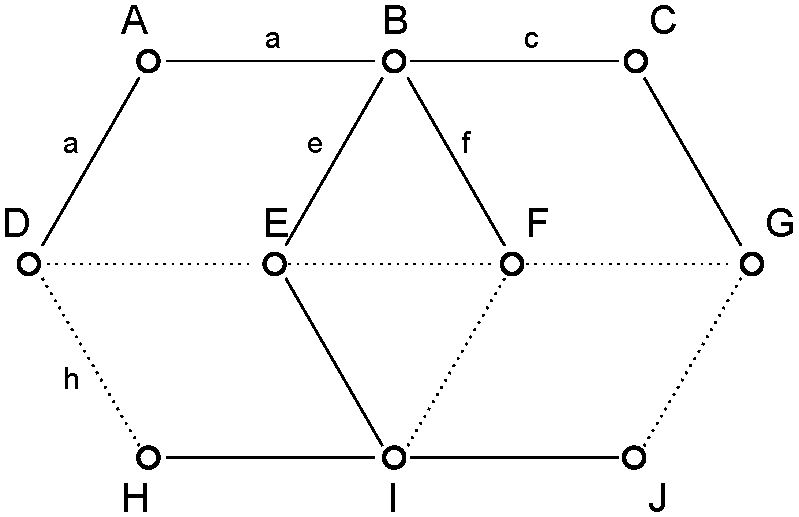
\includegraphics[width=6.5cm]{./images/image37.pdf}
				\begin{tabular}{l|l|l|l|l}
         & A          & B & C        & E                             \\ \hline
					a            & $ t_{Aa} $ & 1 & $ \inf $ & \multicolumn{1}{l|}{$ \inf $} \\ \hline
					e            & $ t_{Ae} $ & 2 & $ \inf $ & \multicolumn{1}{l|}{$ \inf $} \\ \hline
					h            & $ t_{Ah} $ & 4 & $ \inf $ & \multicolumn{1}{l|}{$ \inf $} \\ \cline{2-5} 
				\end{tabular}
				\begin{itemize}
					\item $ t_{Aa} $ - przekazanie pakietu do D z A przez a.
					\item Algorytm nie potrafi wystartować od zera, dlatego na niemożliwe ścieżki wstawia się nieskończoność.
					\item Informacja jest stale aktualizowana. Mówi ona ile czasu potrzeba by wysłac pakiet róznymi ścieżkami.
					\item Przy przesyle w drugą stronę wybiera się trasę najszybszą. Nie musi być to pierwotna $ \rightarrow $ jeśli istnieje inna szybsza, tędy idzie.
					\item Węzeł chce nauczyć się topologii sieci. Zapisuje z każdego przychodzącego pakietu informację o czasie przesyłu. Jeśli nic nie przychodzi to oznacza ścieżkę jako niedostępną.
					\item Węzeł nie posiada szczegółowych informacji o ścieżce, jedynie do którego sąsiada ona prowadzi.
					\item Udowodniono, że zestaw dróg lokalnie optymalnych powinien pokrywać się z trasą globalnie optymalną.
				\end{itemize}
			\subsubsection{Algorytm kooperacyjny z \emph{distance vector}}
				Znany jako algorytm Bellmana-Forda.
				\begin{itemize}
					\item Wymiana metryk tylko z najbliższymi sąsiadami.\\
					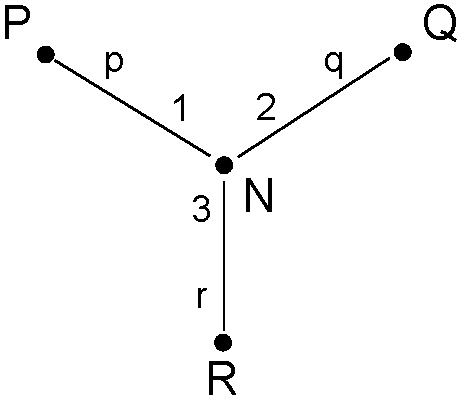
\includegraphics[width=3.5cm]{./images/image40.pdf}\\
					Gdzie:
					\begin{itemize}
						\item Liczby to metryki
						\item Duże litery to adresy
						\item Małe litery to ścieżki
					\end{itemize}
					Można z tego ułożyć ładną początkową tablicę.
					\item Następnie węzeł \emph{N} otrzymuje tablice od sąsiadów oraz dodaje sobie koszt dotarcia do sąsiadów.\\\\
					\begin{tabular}{cccccccc}
						\cline{1-2} \cline{4-5} \cline{7-8}
						\multicolumn{2}{|c|}{\textbf{P}}                                    & \multicolumn{1}{c|}{} & \multicolumn{2}{c|}{\textbf{Q}}                                    & \multicolumn{1}{c|}{} & \multicolumn{2}{c|}{\textbf{R}}                                    \\ \cline{1-2} \cline{4-5} \cline{7-8} 
						\multicolumn{1}{|c|}{Adres} & \multicolumn{1}{c|}{Metryka} & \multicolumn{1}{c|}{} & \multicolumn{1}{c|}{Adres} & \multicolumn{1}{c|}{Metryka} & \multicolumn{1}{c|}{} & \multicolumn{1}{c|}{Adres} & \multicolumn{1}{c|}{Metryka} \\ \cline{1-2} \cline{4-5} \cline{7-8} 
						\multicolumn{1}{|c|}{A}     & \multicolumn{1}{c|}{3}       & \multicolumn{1}{c|}{} & \multicolumn{1}{c|}{B}     & \multicolumn{1}{c|}{3}       & \multicolumn{1}{c|}{} & \multicolumn{1}{c|}{A}     & \multicolumn{1}{c|}{4}       \\ \cline{1-2} \cline{4-5} \cline{7-8} 
						\multicolumn{1}{|c|}{C}     & \multicolumn{1}{c|}{5}       & \multicolumn{1}{c|}{} & \multicolumn{1}{c|}{D}     & \multicolumn{1}{c|}{5}       & \multicolumn{1}{c|}{} & \multicolumn{1}{c|}{B}     & \multicolumn{1}{c|}{7}       \\ \cline{1-2} \cline{4-5} \cline{7-8} 
						\multicolumn{1}{|c|}{D}     & \multicolumn{1}{c|}{7}       & \multicolumn{1}{c|}{} & \multicolumn{1}{c|}{R}     & \multicolumn{1}{c|}{3}       & \multicolumn{1}{c|}{} & \multicolumn{1}{c|}{C}     & \multicolumn{1}{c|}{3}       \\ \cline{1-2} \cline{4-5} \cline{7-8} 
						\multicolumn{1}{|c|}{R}     & \multicolumn{1}{c|}{4}       & \multicolumn{1}{c|}{} & \multicolumn{1}{c|}{S}     & \multicolumn{1}{c|}{5}       & \multicolumn{1}{c|}{} & \multicolumn{1}{c|}{D}     & \multicolumn{1}{c|}{2}       \\ \cline{1-2} \cline{4-5} \cline{7-8} 
						\multicolumn{1}{|c|}{S}     & \multicolumn{1}{c|}{7}       &                       & \multicolumn{2}{c}{+2}                                    &                       & \multicolumn{2}{c}{+3}                                    \\ \cline{1-2}
						\multicolumn{1}{|c|}{Q}     & \multicolumn{1}{c|}{8}       &                       &                            &                              &                       &                            &                              \\ \cline{1-2}
						\multicolumn{2}{c}{+1}                                     & \multicolumn{1}{l}{}  & \multicolumn{1}{l}{}       & \multicolumn{1}{l}{}         & \multicolumn{1}{l}{}  & \multicolumn{1}{l}{}       & \multicolumn{1}{l}{}        
					\end{tabular}
					\item W efekcie czego stacja \emph{N} otrzymuje tablicę możliwości połączeń z innymi, dalszymi stacjami oraz wylicza sobie najkrótsze ścieżki (albo "interfejsy").\\\\
					\begin{table}[h]
						\begin{tabular}{|c|c|l|}
							\hline
							\multicolumn{3}{|c|}{N}                 \\ \hline
							Adres & Metryka & Ścieżka               \\ \hline
							A     & 4       & p                     \\ \hline
							B     & 5       & q                     \\ \hline
							C     & 6       & p                     \\ \hline
							D     & 5       & r                     \\ \hline
							P     & 1       & p                     \\ \hline
							Q     & 2       & q                     \\ \hline
							R     & 3       & r                     \\ \hline
							S     & 7       & q                     \\ \hline
						\end{tabular}
					\end{table}
					\item Wymiana informacji w stałych odstępach czasu, 30 - 60 s, nie za szybko, nie za wolno.
					\item Gdy koszt jest taki sam na dwóch i więcej trasach to teoretycznie można wybrać dowolną z nich.
					\item Adres i metrykę nazywamy wektorem odległości, który jest wysyłany do sąsiadów.
				\end{itemize}
	\section{Uszkodzenia w sieci}
		Wszystkie powyższe algorytmy działają w założeniu, że sieć jest sprawna oraz interesujące nas stacje działają i nie są uszkodzone. Jednak pojawia się kolejny problem: jeżeli któraś ze stacji zostanie uszkodzona i nie może przesyłać wiadomości, inne stacje muszą zostać o tym powiadomione. Analogicznie powinny być informowane o włączaniu stacji do sieci.
		\subsection{Rozchodzenie się informacji}
			\subsubsection{Włączenie stacji}
				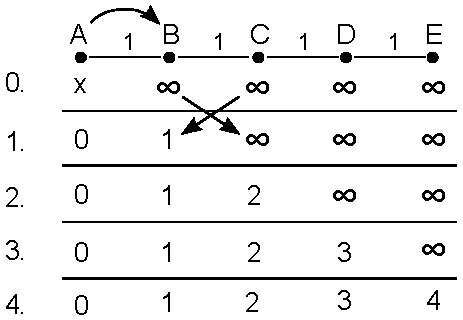
\includegraphics[width=7.0cm]{./images/image42.pdf}
			\subsubsection{Odłączenie stacji}
				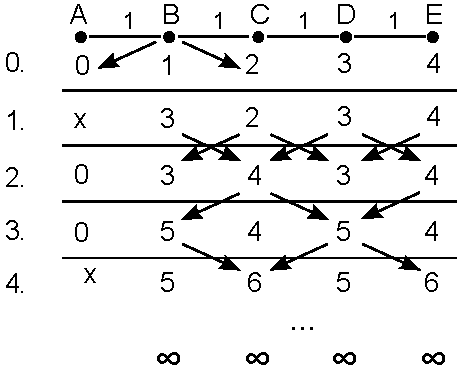
\includegraphics[width=7.0cm]{./images/image43.pdf}\\
				Powoduje liczenie do nieskończoności.
		\subsection{Rozwiązanie - Link State}
			\begin{itemize}
				\item Zasada podziału horyzontów - określanie kierunków
				\item Nie są przesyłane niepotrzebne węzły (?)
				\item Przykładowe łącze\\
				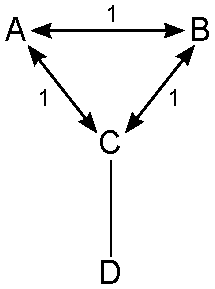
\includegraphics[width=3.0cm]{./images/image44.pdf}
			\end{itemize}
			\subsubsection{Stan łącza}
				\begin{tabular}{|c|l|c|c|}
					\hline
					\multicolumn{3}{|c|}{Nadawca}           & W      \\ \hline
					\multicolumn{4}{|c|}{Nr sekwencyjny}             \\ \hline
					\multicolumn{4}{|c|}{Wiek}                       \\ \hline
					\multicolumn{3}{|c|}{A} & \multicolumn{1}{c|}{1} \\ \hline
					\multicolumn{3}{|c|}{B} & \multicolumn{1}{c|}{3} \\ \hline
				\end{tabular}
				\begin{itemize}
					\item Nr sekwencyjny - jeśli ktoś dostanie pakiet o większym numerze, to go przetwarza, a jeśli nie jest większy, to nie.
					\item Wiek - czas życia pakietu (w cyklu). Jeśli czas życia upływa to węzeł usuwa węzeł W ze swojej tablicy routingu. Liczony w sekundach (chyba)
				\end{itemize}
			\subsubsection{Etapy Link State}
				\begin{enumerate}
					\item "Zapoznaj się z sąsiadami" - wysłanie pakietu HELLO, który zawiera identyfikację nadawcy, oraz czekanie na takie same.
					\item "Wyznacz metrykę trasy" - Echo Request \& Echo Response
					\item Algorytm dystrybucji pakietów LS
					\begin{itemize}
						\item Tworzenie tablicy decyzyjnej routingu (algorytm Dijkstry)\\
						Przykładowa sieć, dane i kierunki dla stacji A.\\
						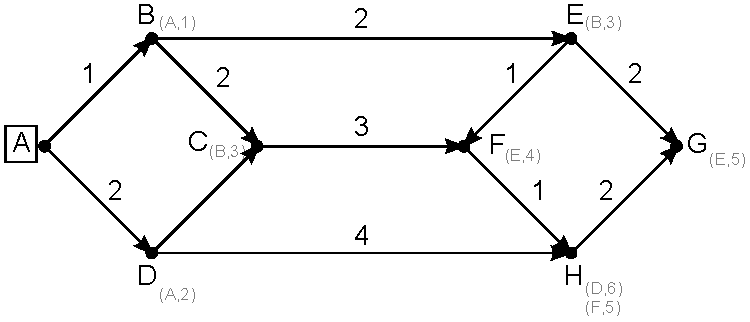
\includegraphics[width=7.0cm]{./images/image45.pdf}\\
						Jeżeli mamy 2 różne wartości, np. $ A\rightarrow D$ - 3, $ A\leftarrow D$ - 2, to przypisujemy średnią.
						\item Tablica routingu\\
						\begin{tabular}{|c|c|}
							\hline
							\multicolumn{1}{|c|}{\textbf{Adres}}           & \textbf{Droga}      \\ \hline
							\multicolumn{1}{|c|}{B}               & b          \\ \hline
							\multicolumn{1}{|c|}{C}               & b          \\ \hline
							\multicolumn{1}{|c|}{D}               & d          \\ \hline
							\multicolumn{1}{|c|}{E}               & b          \\ \hline
							\multicolumn{1}{|c|}{F}               & b          \\ \hline
							\multicolumn{1}{|c|}{G}               & b          \\ \hline
						\end{tabular}
						\item Zmiany w topologii są rozsyłane natychmiast - nie ma liczenia do nieskończoności.
						\item Algorytm co jakiś czas wykonuje się ponownie (odświeżanie).
					\end{itemize}
				\end{enumerate}
	\section{Problemy z liczbą węzłów}
		\subsection{Metoda hierarchii}
			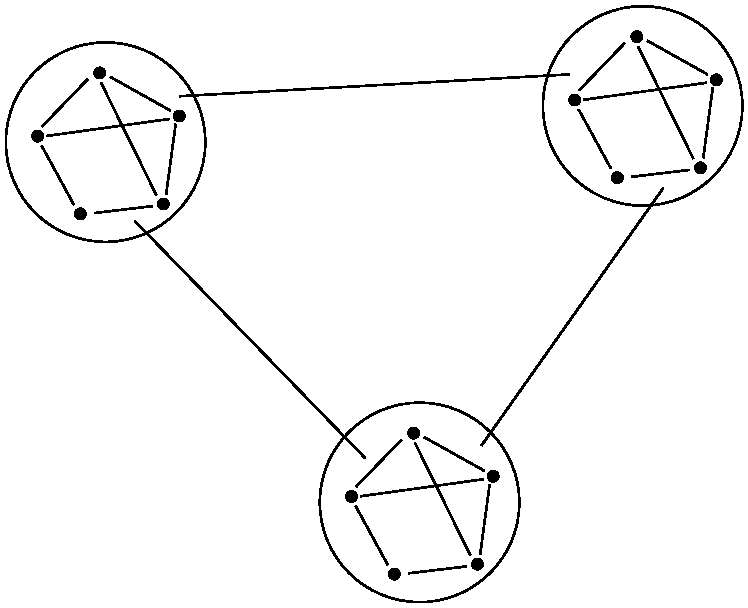
\includegraphics[width=7.0cm]{./images/image46.pdf}\\
			Jest tylko 1 wpis na całą sieć w tabeli routingu.\\
			Zawiera wpisy na połączenia lokalne.
		\subsection{Inny sposób}
			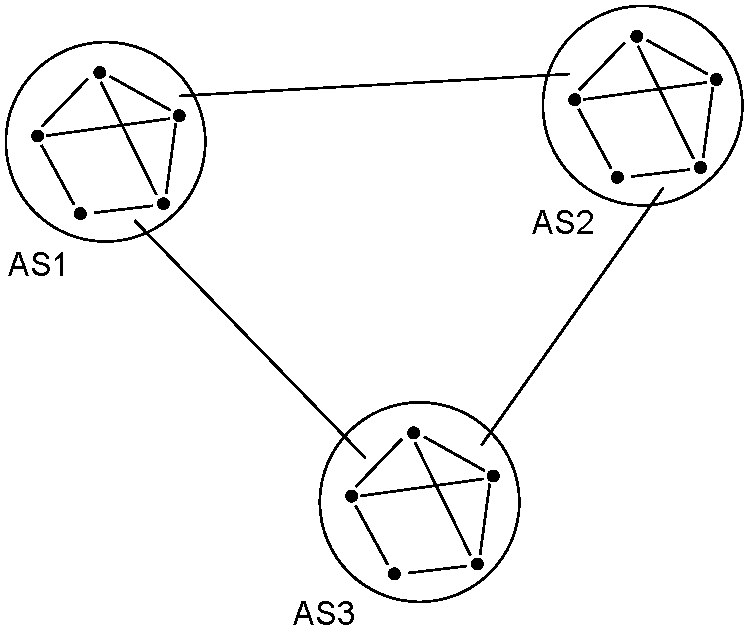
\includegraphics[width=7.0cm]{./images/image47.pdf}\\
			System autonomiczny. AS1 - AS3 (mogą to być firmy, instytucje itp.) traktujemy jako osobne węzły, więc rysunek można uprościć do postaci zwykłego trójkąta.
		\subsection{Routery}
			Dzielimy je na:
			\begin{itemize}
				\item Zewnętrzne - EGP (External Gateway Protocol)
				\item Wewnętrzne - IGP (Internal ...)
			\end{itemize}
			IGP działa dla routingu w najbliższym sąsiedztwie, natomiast EGP ustala zasady routingu między sąsiedztwami.
		\subsection{Przeciążenie Sieci}
		
		\subsubsection{Oznaki przeciążenia sieci }
			Wcześniej muszą zostać zdefiniowane (którego używamy).
			\begin{itemize}
				\item Przeciętna długość przerwy pomiędzy transmisją kolejnych pakietów.
				\item Retransmisja pakietu ze względu na timeout
				\item Przeciętna długość que[ry] (???)
			\end{itemize}
				\subsubsection{Poziomy zagrożenia}
				\begin{itemize}
					\item Dzielą się na: zielony, żółty, pomarańczowy, czerwony. Osiągnięcie pomarańczowego poziomu zazwyczaj oznacza problemy w sieci.
					\item Inna notyfikacja: Overload Forward Congestion Notification (OFCN) - obliczana procentowo. Kolejne poziomy obciążenia obliczane są od górnej granicy (100\%, 50\%, 25\%...)
				\end{itemize}
			\subsubsection{Ogólna zasada działania}
				Generowana jest pula wolnych biletów. W sieci może krążyć tylko tyle pakietów, ile jest woolnych biletów. Następne pakiety muszą czekać, aż zwolni się jakiś bilet. Po upływie pewnego czasu generowana jest nowa pula biletów.
			\subsubsection{Algorytmy zapobiegające obciążeniu}
				\begin{itemize}
					\item Random Error Discard/Detection (RED) - wyrzuca się losowe pakiety, żeby zmniejszyć tłok na łączu.
					\item Error Recovery (algorytm retransmisji) - Aktywowany, kiedy pakiety przestają się mieścić w czasie timeoutu. Tworzy się retransmisję lub retransmisję selektywną (konkretnego pakietu) - jeżeli ponownie nie trafi z pakietem, to jeszcze bardziej obciąży sięć.
				\end{itemize}
			
\part{Protokoły}
% =========================================
% Lolnotatki 08.01.15
% =========================================
\subsection{IPv4}

\subsubsection{Klasy IP}
\begin{itemize}
	\item Nazwa Klasy - zapis / maska bitów 
	\item A = 10.000 / 8
	\item 16-B 172.16 - 31.255.255 / 12
	\item B 192.168.0.0 / 16
\end{itemize}
\subsubsection{Transport}
\begin{table}[h]
	\begin{tabular}{|c|c|}
		\hline
		IP	&	Port (16)	\\ \hline
	\end{tabular}
\end{table}
APIPA \emph{Automatic Private IP Assigned} - algorytm uruchamiany, kiedy system nie może pobrać adresu z sieci, a ma pobrać adres z sieci.
169.254.0.0 - generowany jest losowy adres, który przepisywany jest systemowi. Komputery, które sa odłączone od sieci automatycznie konfigurują się tym algorytmem. Kiedys komputery nie mogły sie uruchamiac bez adresu.\\
Broadcast, przykład:
\begin{table}[h]
	\begin{tabular}{|c|c|}
		\hline
		27(maska) &	5	\\ \hline
	\end{tabular}
\end{table}
\begin{itemize}
	\item 00000 - Network
	\item 11111 - Broadcast
\end{itemize}



\subsection{IPv6}
Rozmiar 128 bitów, znacznie więcej niż w IPv4.

\begin{table}[h]
	\begin{tabular}{|l|l|l|l|l|}
		\hline
		ver       & PRID       & \multicolumn{3}{l|}{Etykieta przepływowa}      \\ \hline
		\multicolumn{3}{|l|}{Długość danych} & Next Header      & HopLimit      \\ \hline
		\multicolumn{5}{|l|}{SourceAddress (128 bit)}                           \\ \hline
		\multicolumn{5}{|l|}{Destination Address}                               \\ \hline
	\end{tabular}
\end{table}
1: 0, 2, 24, 31\\
2: 8, 8, 8\\
Next headers:
\begin{itemize}
	\item Hop by hop options - opcje wykonywane w kolejnych krokach
	\item Routing
	\item Fragmentation
	\item Authentication
	\item Destionation options
	\item Encryption security payload
	\item Jumbo header - nagłówek sygnalizujący specjalny rozmiar pakietu, ~1 MB.
\end{itemize}
\textbf{Routing}\\
Next Header określa rodzaj.\\
\begin{table}[h]
	\begin{tabular}{|l|l|l|l|l|}
		\hline
		Next header & Pole związane z nagłówkiem & \multicolumn{3}{l|}{Kod opcji (i1ość adresów + network adres)} \\ \hline
		x           & \multicolumn{4}{l|}{BitMap}                                                                 \\ \hline
		\multicolumn{5}{|l|}{}                                                                                    \\ \hline
		\multicolumn{5}{|l|}{1 do 24 Adres IPv6}                                                                  \\ \hline
	\end{tabular}
\end{table}

\textbf{Jumbo}\\
Dla środowiska superkomputerów
\begin{table}[h]
	\begin{tabular}{|l|l|l|l|l|}
		\hline
		Next header & Pole związane z nagłówkiem & 194 & \multicolumn{2}{l|}{} \\ \hline
		\multicolumn{5}{|l|}{Jumbo payload size}                               \\ \hline
	\end{tabular}
\end{table}
RFC 1883 - 1887.

\begin{itemize}
	\item Unicast address - do jednego
	\item Multicast address - do wielu
	\item Anycast address - do jednego z wielu (w obrębie grupy)
\end{itemize}

2001:cdba:0000:0000:0000:0000:3257:9652 - pełny 128-bitowy adres IP.\\
CDBA - heksadecymalnie, określają 4 grupy.\\
W zapisie grupa 4 zer może być zapisana jednym zerem.\\
2001:cdba:0:0:0:0:3257:9652\\
2001:cdba::3257:9652

\subsubsection{Specjalne adresy IPv6}
\begin{itemize}
	\item \textbf{::/96} - adres zgodny z zapisem IPv4
	\item \textbf{::/128} - odpowiednik adresu IP składającego się z samych zer i oznacza sieć nieokreśloną (\emph{Unspecified Address}).
	\item \textbf{::1/128} - adresem local loopback jest adres składający się z samych zer i jednej jedynki.
	\item \textbf{2001:db8::/32} - \emph{documentation prefix}
	\item \textbf{fec0::/10} - \emph{side local prefix} - dla pierwszych 16 bitów, jeżeli są one w tym, to definiuje adresy uzywane wewnątrz danej lokalizacji.
	\item \textbf{fc00::/7} \emph{unic local address}
	\item \textbf{ff00::/8}
	\item \textbf{ff80::/10} - adres przydzielony w łączu (\emph{link local prefix})
\end{itemize}

\subsection{Protokoły}
\subsubsection{TCP}
\begin{table}[h]
	\begin{tabular}{|c|c|c|c|c|}
		\hline
		\multicolumn{5}{|l|}{Source IP}                 \\ \hline
		\multicolumn{5}{|l|}{Destination IP}                 \\ \hline
		\multicolumn{2}{|l|}{Source port} & \multicolumn{3}{l|}{Destination port}                \\ \hline
		\multicolumn{5}{|l|}{Nr sekwencyjny pakietu}                                             \\ \hline
		\multicolumn{5}{|l|}{nr potiwerdzenia pakietu}                                           \\ \hline
		TCP header length       & x       & Flagi          & \multicolumn{2}{l|}{Window Size}    \\ \hline
		\multicolumn{3}{|l|}{Suma kontrolna}               & \multicolumn{2}{l|}{Urgend pointer} \\ \hline
		\multicolumn{5}{|l|}{OPCJA}  \\ \hline
		\multicolumn{5}{|l|}{SAC}  \\ \hline
	\end{tabular}
\end{table}

\subsubsection{UDP}
\begin{table}[h]
	\begin{tabular}{|l|l|l|l|l|}
		\hline
		\multicolumn{2}{|l|}{Source port}   & \multicolumn{3}{l|}{Destination port} \\ \hline
		\multicolumn{2}{|l|}{Packet length} & \multicolumn{3}{l|}{Suma kontrolna}   \\ \hline
	\end{tabular}
\end{table}

\textbf{Flagi i komendy UDP}:
\begin{itemize}
	\item URG
	\item ACK
	\item PSH
	\item RST
	\item SYN
	\item FIN
\end{itemize}

\textbf{Algorytmy, które wymuszają pewne mechanizmy zapobiegające przeciążeniu sieci}. odpowiadają za zabezpieczenie transportu z warstwy trzeciej do warstwy czwartej - gubieniu pakietów.
\begin{itemize}
	\item slow start
	\item congestion avoidance
	\item multiplicative descrease
\end{itemize}

Obrazek: slow start
Uzgodniony rozmiar okna (z odbiorcą), którego nie możemy przekroczyć.


% === ZADANIA
% !TeX spellcheck = pl_PL

\newpage
\begin{center}
	{\LARGE \textbf{k - 1000, K - 1024 !!!}}
\end{center}

\part{Zadania}
% ==================================================
% --- 1. TOPOLOGIA SIECI
% ==================================================
\section{Topologia sieci}
	% ================= ZADANIE 1.1 ==================
	\subsection{Zadanie}
		\subsubsection{Treść}
			\begin{wrapfigure}{l}{6.0cm}
				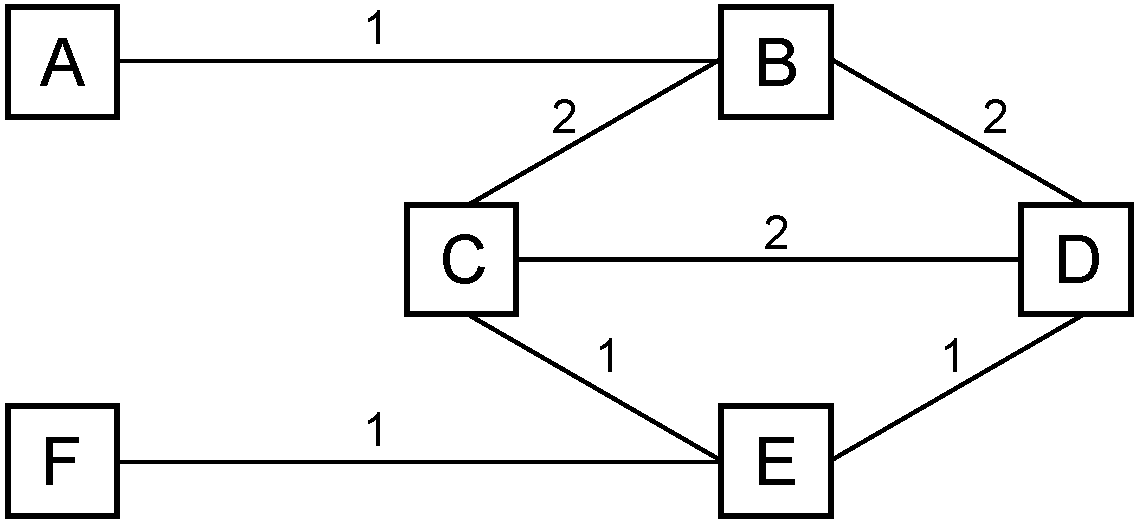
\includegraphics[width=5.5cm]{./images/zadanie02.pdf}
			\end{wrapfigure} 
			W sieci z metryką jak na rysunku routery wymieniają się informacjami co 40 sekund, stosowany jest protokół typu Distance Vector. W chwili $ t_0 $ router F ulega awarii. Określ, po jakim czasie informacja o niedostępności routera F dotrze do węzła A.\\\\\\\\
		\subsubsection{Odpowiedź}
			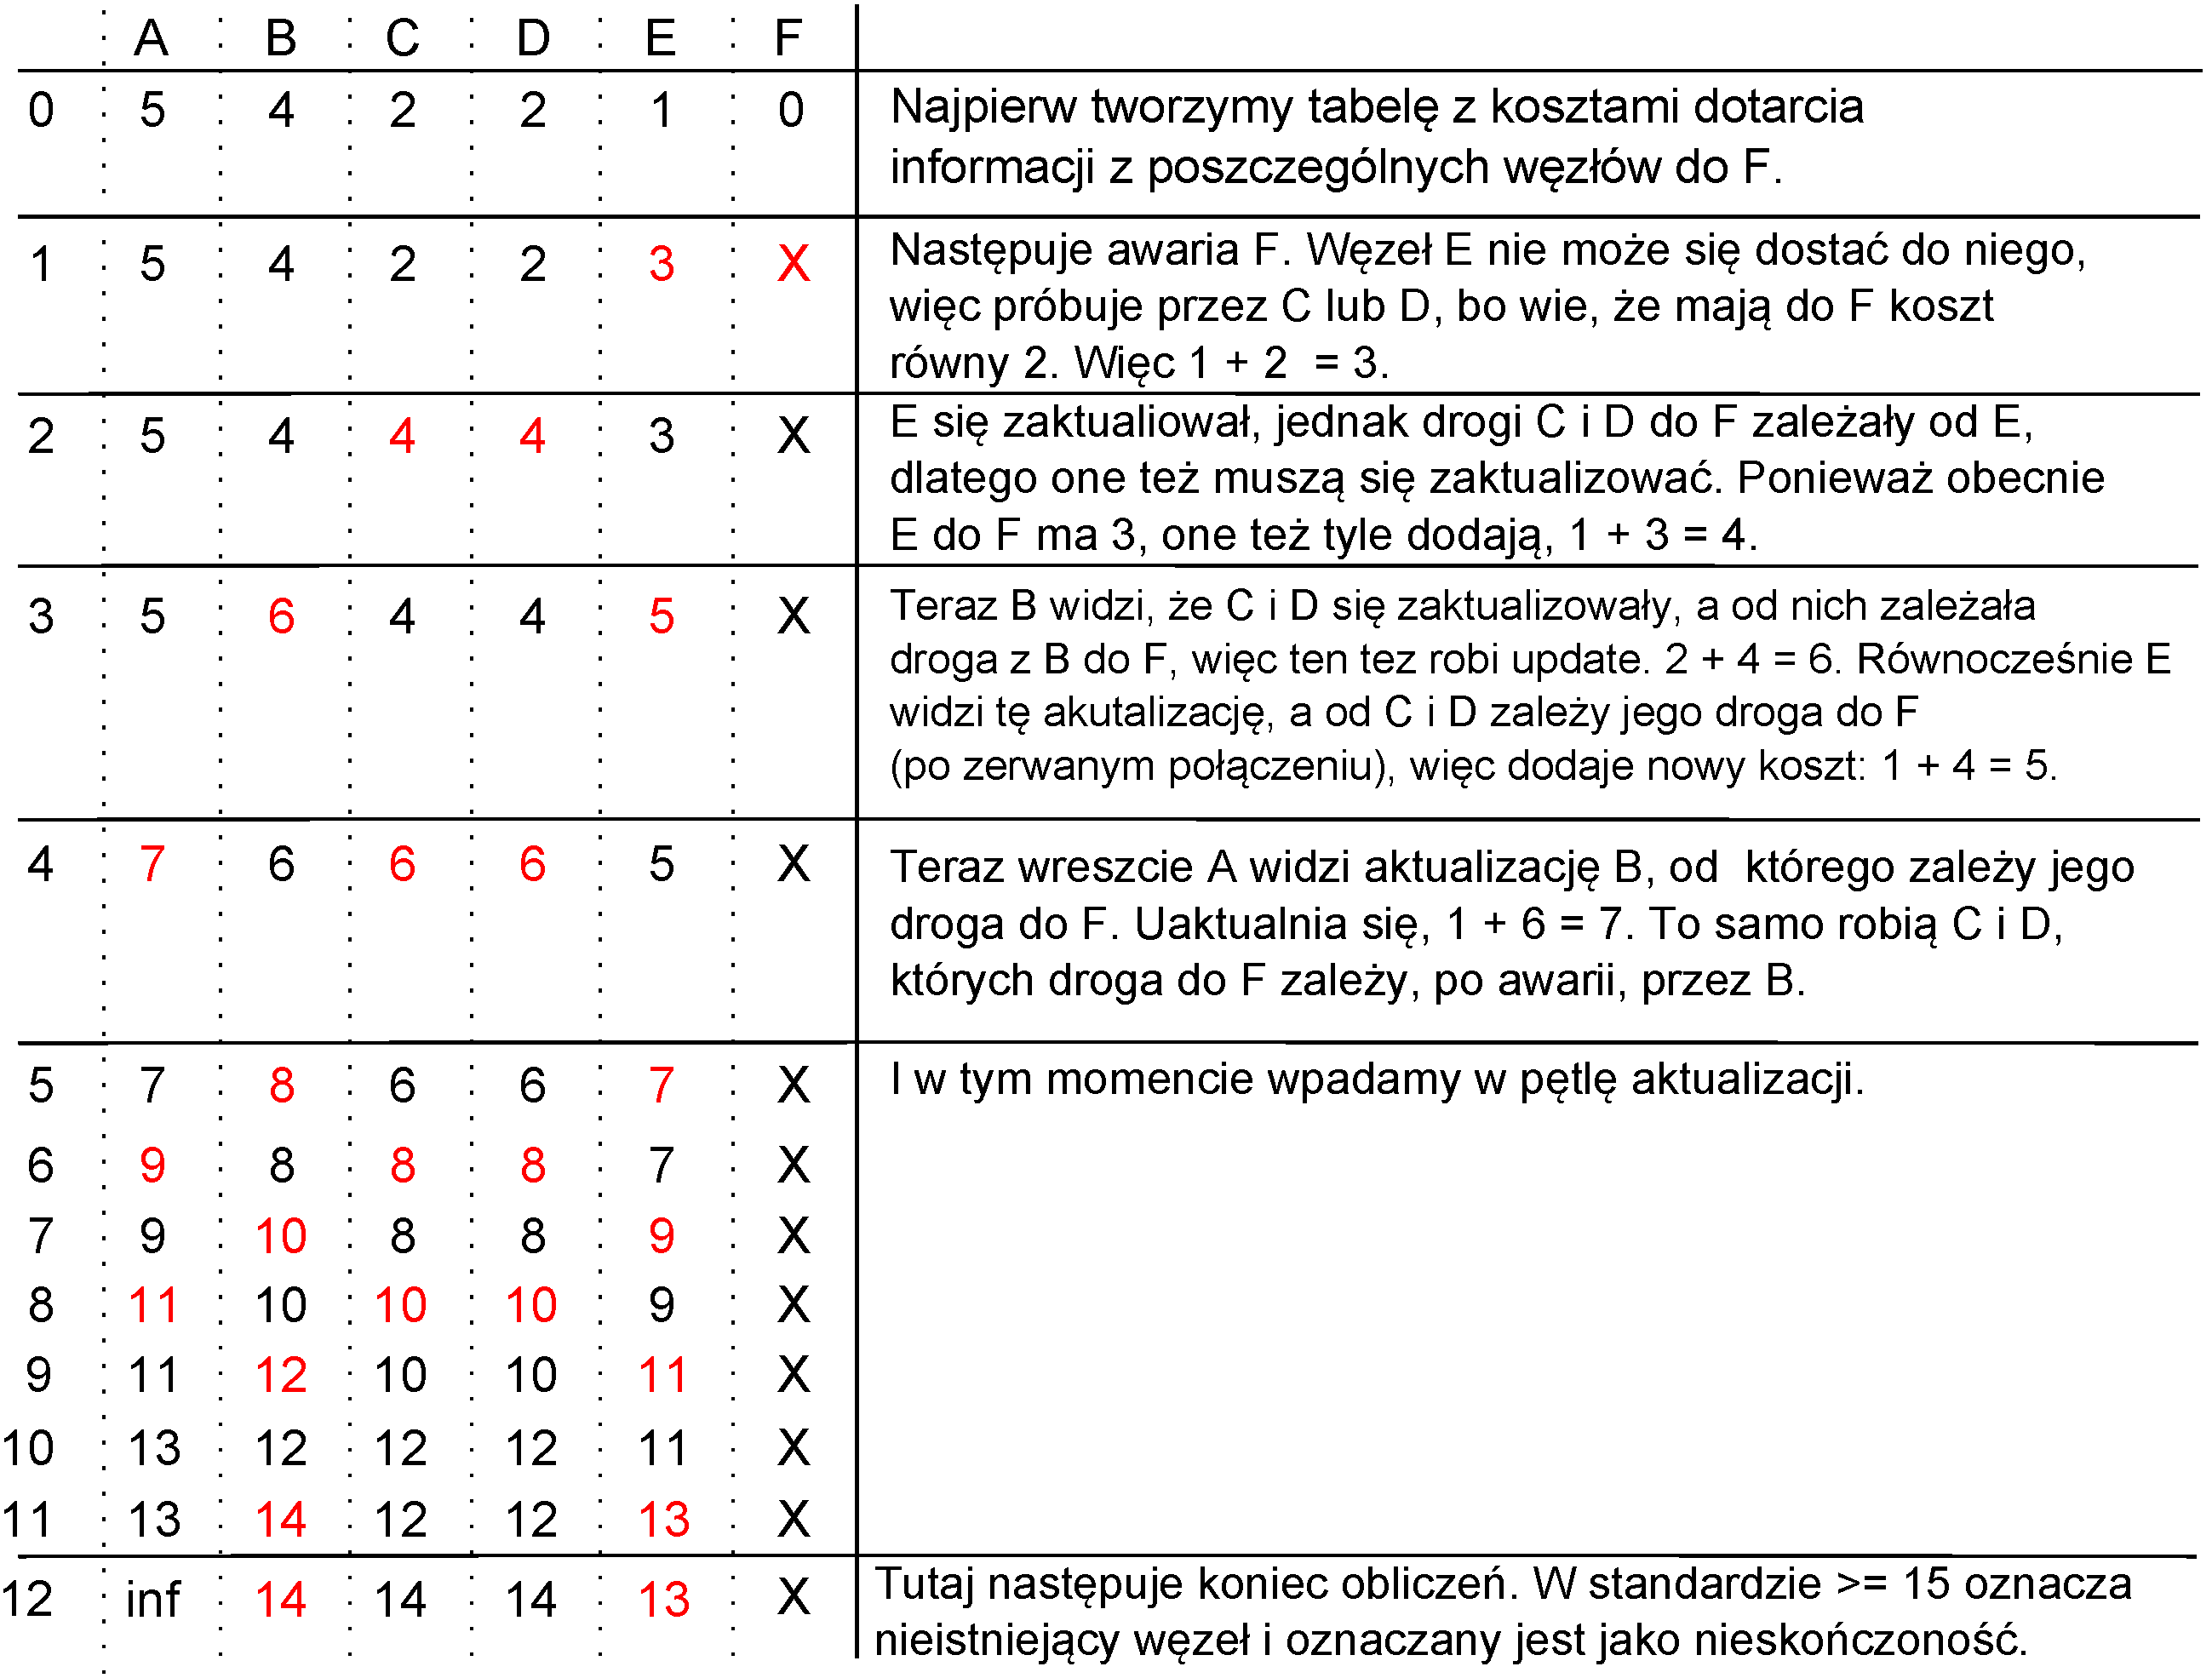
\includegraphics[width=16.0cm]{./images/zadanie03.pdf}\\
			A więc stacja A dowie się o niedostępności stacji F po $ 12\cdot 40\;s=480\;s $.
\newpage
	% ================= ZADANIE 1.2 ==================
	\subsection{Zadanie}
		\subsubsection{Treść}
			Dana jest następująca topologia sieci:
			\begin{itemize}
				\item Węzeł B ma jako sąsiadów węzły A, C i D
				\item Węzeł C ma jako sąsiadów węzły A, B, D i E
				\item Węzeł D ma jako sąsiadów węzły A, B, C i E
				\item Węzeł E ma jako sąsiadów węzły C i D
			\end{itemize}
			W chwili $ t_0 $ węzeł B ulega awarii. Przedstaw sposób rozchodzenia się tej informacji między węzłami, po jakim czasie informacja o tym dotrze do węzła E, jeśli w sieci stosowany jest protokół RIP typu Distance Vector i cykl wymiany wektorów wynosi 30 s. Przyjmij metrykę jednostkową łączy.
		\subsubsection{Odpowiedź}
			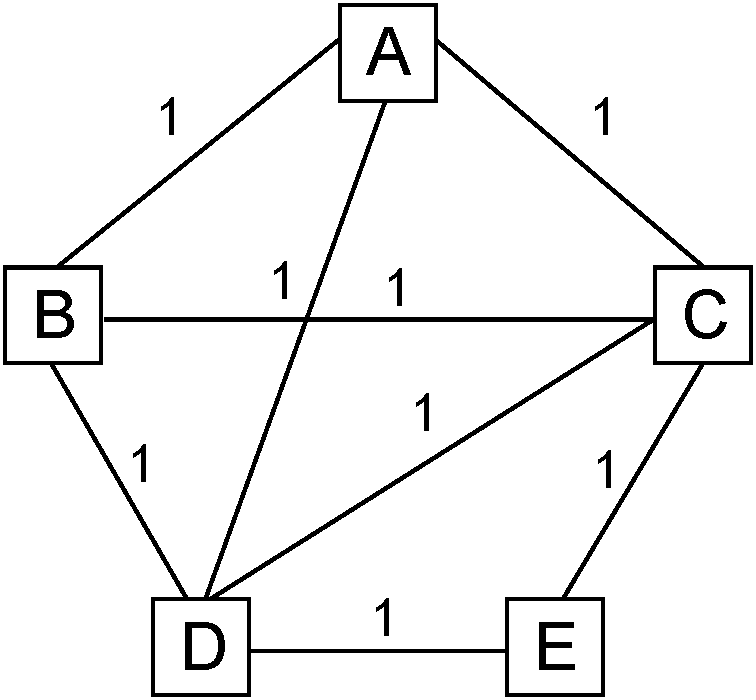
\includegraphics[width=5.0cm]{./images/zadanie04.pdf}\\\\
			\begin{tabular}{|c|c|c|c|c|c|p{7cm}|}
				\hline \textbf{Zmiana} & \textbf{A} & \textbf{B} & \textbf{C} & \textbf{D} & \textbf{E} & \textbf{Komentarz} \\ 
				\hline \textbf{-} & 1 & 0 & 1 & 1 & 2 & Działa \\ 
				\hline \textbf{0} & \color{red}{inf} & \color{red}{X} & \color{red}{inf} & \color{red}{inf} & 2 & B ulega awarii. Sąsiedzi, czyli A, C i D nie mogą się połączyć z nim. \\ 
				\hline \textbf{1} & \color{red}{4} & X & \color{red}{3} & \color{red}{3} & 2 & Węzły A, B i C próbują się połączyć z B przez E, który nie wie o awarii. \\ 
				\hline \textbf{2} & 4 & X & 3 & 3 & \color{red}{4} & Ponieważ droga z węzła E do B pierwotnie wiodła przez węzły D i C, po ich zmianie ich tablic, E również musi je aktualizować, nawet pomimo tego, że obecna droga C i D wiedzie przez niego (nie wie o tym). \\
				\hline \textbf{3} & \color{red}{6} & X & \color{red}{5} & \color{red}{5} & 4 & I zaczyna się pętla. \\ 
				\hline \textbf{4} & 6 & X & 5 & 5 & \color{red}{6} &  \\ 
				\hline \textbf{5} & \color{red}{8} & X & \color{red}{7} & \color{red}{7} & 6 &  \\ 
				\hline \textbf{6} & 8 & X & 7 & 7 & \color{red}{8} &  \\ 
				\hline \textbf{7} & \color{red}{10} & X & \color{red}{9} & \color{red}{9} & 8 &  \\ 
				\hline \textbf{8} & 10 & X & 9 & 9 & \color{red}{10} &  \\ 
				\hline \textbf{9} & \color{red}{12} & X & \color{red}{11} & \color{red}{11} & 10 &  \\ 
				\hline \textbf{10} & 12 & X & 11 & 11 & \color{red}{12} &  \\ 
				\hline \textbf{11} & \color{red}{14} & X & \color{red}{13} & \color{red}{13} & 12 &  \\ 
				\hline \textbf{12} & 14 & X & 13 & 13 & \color{red}{14} &  \\ 
				\hline \textbf{13} & \color{red}{16} & X & \color{red}{15} & \color{red}{15} & 14 &  \\ 
				\hline \textbf{14} &  &  &  &  & \color{red}{16} & Koniec \\ 
				\hline 
			\end{tabular}\\\\
			Obliczenia kończą się, gdy koszt trasy z węzła E do B przekroczy 15. Wówczas widzimy, że dokonanych zmian było 14, a więc czas wynosi: $ 14\cdot 30\;s=420\;s=7$ minut.

% ==================================================
% --- 2. ETHERNET
% ==================================================
\section{Ethernet}
	% ================= ZADANIE 2.1 ==================
	\subsection{Zadanie}
		\subsubsection{Treść}
			Kontroler karty sterownika sieci Ethernet odebrał następujące ramki:
			\begin{enumerate}
				\item Długość 51 bajtów, poprawne CRC
				\item Długość 39 bajtów, błędne CRC
				\item Długość 66 bajtów, poprawne CRC
				\item Długość 1510 bajtów, poprawne CRC
				\item Długość 1525 bajtów, poprawne CRC
				\item Długość 1540 bajtów, błędne CRC
			\end{enumerate}
			Jak zaklasyfikować powyższe ramki? (błąd protokołu, błąd transmisji, kolizja, poprawna ramka)
		\subsubsection{Odpowiedź}
			\begin{itemize}
				\item Jeśli ramka ma mniej niż 64 bajty i błędne CRC to jest to kolizja
				\item Jeśli ramka ma mniej niż 64 bajty i poprawne CRC to jest to błąd protokołu
				\item Jeśli ramka ma więcej niż 1518 bajtów, to zawsze jest to błąd protokołu, niezależnie od poprawności CRC
				\item Jeśli ramka ma niemniej 64 bajty i nie więcej niż 1518 bajtów oraz niepoprawne CRC to jest to błąd transmisji
				\item Poprawna ramka powinien mieć 64 - 1518 bajtów i poprawne CRC
			\end{itemize}
			\begin{enumerate}
				\item Błąd protokołu
				\item Kolizja
				\item Poprawna
				\item Poprawna
				\item Błąd protokołu
				\item Błąd protokołu
			\end{enumerate}
	% ================= ZADANIE 2.2 ==================
	\subsection{Zadanie}
		\subsubsection{Treść}
			W przypadku wystąpienia kolizji w segmencie sieci Ethernet czas oczekiwania na retransmisję $ T_R $ generowany jest jako liczba losowa z przedziału:
			\begin{enumerate}
				\item O stałej wielkości ustalanej przy konfiguracji sieci (jakiej?)
				\item O wielkości rosnącej liniowo z numerem kolizji
				\item O wielkości rosnącej z kwadratem numeru kolizji
				\item O wielkości rosnącej z kwadratem do pewnego numeru kolizji
			\end{enumerate}
			Jak obliczany jest czas $ T_R $?
		\subsubsection{Odpowiedź}
			Chodzi tutaj o algorytm CSMA, wykorzystywany do rozwiązywania kolizji na łączu kablowym. Wzór, o który prosi pytanie, zawarty jest w algorytmie dostępu w transmisji częściowo kontrolowanej. W pełni kontrolowanym dostępie występuje Token oraz rywalizacja stacji o dostęp (chyba o to chodzi).
			$$ T_{R} = r(x)\times (2^{k}-1)\times T_{ob}$$Gdzie:
			\begin{itemize}
				\item $ r(x) $ - liczba losowa z zakresu 0...1
				\item $ T_{ob} $ - czas obiegu łącza, w najgorszym wypadku podwojony czas propagacji
				\item $ k $ - liczba kolizji, czyli który raz się te ramki już zderzyły.
				\item Wraz ze zwiększaniem się liczby kolizji, możliwy zakres rośnie ekspotencjalnie. Jednak maksymalna wielkość $ k $ jest równa \textbf{10}. Dla $ k > 10 $ przyjmuje się $ k=10 $.
				\item Próbujemy szczęścia aż $ k < 15 $, potem próby są przerywane.
			\end{itemize}
			Dlatego poprawna odpowiedź to: \textit{Czas oczekiwania na retransmisję $ T_R $ generowany jest jako liczba losowa z przedziału \textbf{o wielkości rosnącej z kwadratem do pewnego numeru kolizji, \underline{a tym numerem jest 10}}}\\
			{\small \emph{Forczu: jeszcze to sprawdzę}}.
	% ================= ZADANIE 2.3 ==================
	\subsection{Zadanie}
		\subsubsection{Treść}
			Chcemy zastosować protokół CSMA / CD przy budowie sieci o długości łącza 500 m przy szybkości transmisji 200 MBit/s. Jaka powinna być w tym przypadku minimalna długość ramki?
		\subsubsection{Odpowiedź}
			Najpierw liczymy czas propagacji $$ t_p = \cfrac{dystans}{predkosc\_lacza} $$
			Prędkości łącza nie mylić z szybkością transmisji. W przypadku światłowodu wynosi ono 2/3 prędkości światła czyli 200 000 000 m/s, tu takie założenie można dać. O tej wartości należy pamiętać na sztywno. Następnie liczmy czas propagacji sygnału przez 500 [m]:
			$$ t_p=\frac{500\;[m]}{200\:000\:000\:[m/s]}=2.5\:\mu s $$
			W obie strony czas ten wynosi $ 2.5\:\mu s = 5\:\mu s$.\\
			Bierzemy czas 2 razy, ponieważ "istnieje możliwość, że dwa lub więcej urządzeń przystąpi do wysyłania danych w tej samej chwili lub zanim sygnał z pierwszego węzła dotrze do drugiego. W takiej sytuacji żadne z nich nie wykryje sygnału nośnego drugiego. W efekcie obydwa urządzenia wysyłając dane w (prawie) tym samym czasie spowodują kolizję w sieci Ethernet."\\
			Aby CSMA/CD działało poprawnie cała ramka musi być wysłana w tych $5\:\mu s$, czyli wyliczamy jej długość:
			$$ N=szybkosc\_transmisji\cdot t_p $$
			$$ N=200\:000\:000\:[bit]\cdot \frac{5}{10^6} =200\cdot5=1000\:bit=125\:B $$
			
% ==================================================
% --- 3. TCP / IP
% ==================================================
\section{TCP / IP}
% ================= ZADANIE 3.1 ==================
\subsection{Zadanie}
	\subsubsection{Treść}
		Przedstaw i porównaj dostępne mechanizmy działania protokołu sterowania przypływem w połączeniach warstwy transportowej i w połączeniach warstwy liniowej (np. SDLC, TCP). W jaki sposób odbierająca stacja transportowa może uzyskać czasowe powstrzymanie transmisji przez nadawcę?
	\subsubsection{Odpowiedź}
		\begin{itemize}
			\item \textbf{TCP} - kontrolowanie poprzez zmianę rozmiaru okna odbiorcy.
			\item \textbf{SDLC / HDLC} - kontrolowanie przez sygnały typu WACK / ACK w protokole znakowym BSC (RR, RNR).
		\end{itemize}

% ==================================================
% --- 4. ROUTING
% ==================================================
\section{Routing}
	% ================= ZADANIE 4.1 ==================
	\subsection{Zadanie}
		\subsubsection{Treść}
			Opisz zasadę działa algorytmu dystrybucji pakietów Link State. Przedstaw działanie algorytmu w węźle A w przypadku, gdy węzeł ma jako sąsiadów węzły B, C, D, E i F oraz otrzymał w czasie ostatnich 5 ms pakiety z węzłów C, F i D. Przyjąć, że maksymalny czas oczekiwania na kolejne kopie to 10 ms i węzeł nie odebrał w tym czasie innych pakietów.
		\subsubsection{Odpowiedź}
				\begin{tabular}{|c|c|c|c|c|c|c|c|}
					\hline \multicolumn{2}{|c|}{\textbf{C}}  & & \multicolumn{2}{|c|}{\textbf{F}} & & \multicolumn{2}{|c|}{\textbf{D}}\\ 
					\hline \multicolumn{2}{|c|}{213} & &\multicolumn{2}{|c|}{214} & &\multicolumn{2}{|c|}{214} \\ 
					\hline \multicolumn{2}{|c|}{178} & &\multicolumn{2}{|c|}{260} & &\multicolumn{2}{|c|}{259}   \\ 
					\hline U & 3 & & U & 2 & & U & 2\\ 
					\hline V & 5 & & V & 4 & & V & 4\\
					\hline Z & 4 & & Z & 5 & & Z & 5\\
					\hline 
				\end{tabular}\\\\\\
			Przykładowy zestaw pakietów zadziała następująco: stacja A wyśle potwierdzenia do węzłów F i D. Do węzłów B, C i E wyśle pakiet z F. Dlaczego?\\
			Potwierdzenia wysyłane są do węzłów z których przyszły pakiety z najwyższym numerem sekwencyjnym (drugi wiersz). W tym przypadku są to węzły F i D, których $ seq $ są równie 214. Do sąsiadów, którzy nie otrzymali potwierdzenia (B, C i E) wysyłany jest ten spośród pakietów z najwyższym numerem sekwencyjnym, którego pole Age (trzeci wiersz) jest największe. Dlatego co tych trzech węzłów zostanie wysłany pakiet z F.
\newpage
	% ================= ZADANIE 4.2 ==================
	\subsection{Zadanie}
		\subsubsection{Treść}
			Węzeł W ma za sąsiadów węzły A, B, C, D i E. Po otrzymaniu pakietu Link State węzeł oczekuje 35 ms, następnie przystępuje do dystrybucji pakietu. W chwili $ t_0 $ węzeł odebrał pakiet z węzła B, $ 5\;ms $ później z węzła D, a po 13 $ ms $ pakiet z węzła E. Przedstaw przebieg dystrybucji pakietów\\.
			\begin{tabular}{|c|c|c|c|c|c|c|c|}
				\hline \multicolumn{2}{|c|}{\textbf{E}}  & & \multicolumn{2}{|c|}{\textbf{B}} & & \multicolumn{2}{|c|}{\textbf{D}}\\ 
				\hline \multicolumn{2}{|c|}{55} & &\multicolumn{2}{|c|}{55} & &\multicolumn{2}{|c|}{55} \\ 
				\hline \multicolumn{2}{|c|}{240} & &\multicolumn{2}{|c|}{238} & &\multicolumn{2}{|c|}{239}   \\ 
				\hline U & 2 & & U & 1 & & U & 2\\ 
				\hline V & 3 & & V & 2 & & V & 3\\
				\hline Z & 6 & & Z & 5 & & Z & 6\\
				\hline 
			\end{tabular}
		\subsubsection{Odpowiedź}
			Do węzłów, których pakiety miały największy nr sekwencyjny (2gi wiersz) wysyła potwierdzenie
			Do pozostałych wysyła pakiet tego węzła, który miał największy nr sekwencyjny i age (3ci wiersz).
			\begin{itemize}
				\item Do węzła D wyśle: potwierdzenie.
				\item Do węzła C wyśle: E.
				\item Do węzła B wyśle: potwierdzenie.
				\item Do węzła E wyśle: potwierdzenie.
				\item Do węzła A wyśle: E.
			\end{itemize}
	% ================= ZADANIE 4.3 ==================
	\subsection{Zadanie}
		\subsubsection{Treść}
			\begin{wraptable}{r}{5.5cm}
				\begin{tabular}{|c|c|}
					\hline \multicolumn{2}{|c|}{Q}  \\ 
					\hline \multicolumn{2}{|c|}{1}  \\ 
					\hline \multicolumn{2}{|c|}{300}  \\ 
					\hline T & 2 \\ 
					\hline U & 1 \\ 
					\hline Z & 3 \\ 
					\hline 
				\end{tabular}
			\end{wraptable}
			Węzeł Q generuje co 60 sekund pakiety Link State, w chwili $ t_0 $ rozesłał pakiet
			$$ (Q\;|\;seq=23321\;|\;age=300\;|\;(U|3)\;|\;(V|2)\;|\;(Z|5)\;) $$
			Po restarcie w chwili $ t_0+25\;s $ wysłał pakiet
			$$ (Q\;|\;seq=1\;|\;age=300\;|\;(T|2)\;|\;(U|1)\;|\;(Z|3)\;) $$
			a potem kolejne. Przedstaw przebieg dystrybucji tej informacji w sieci. Kiedy te zmiany w topologii zostaną uwzględnione w wyznaczaniu tablicy routingu?
		\subsubsection{Odpowiedź}
			Działanie Link State:
			\begin{itemize}
				\item "Powiedz wszystkim o swoich sąsiadach" - przekazuje pakiety otrzymane od sąsiednich węzłów do sąsiednich węzłów.
				\item Nr sekwencyjny - jeśli ktoś dostanie pakiet o większym numerze, to go przetwarza (i przesyła dalej), a jeśli nie jest większy, to nie.
				\item Wiek - czas życia pakietu (w cyklu). Jeśli czas życia upływa to jest usuwany z tablicy routingu. Liczony w sekundach.
			\end{itemize}
\newpage
			\textbf{Odpowiedzi}:
			\begin{enumerate}
				\item Węzły odrzucają pakiet z niższym numerem sekwencyjnym, więc nowy pakiet będzie uwzględniony po wygaśnięciu wa(żności?) pierwszego, czyli za $ 275\;s $.\\
				\small{ \emph{Ocenione na 0.9 / 1.0}}
				\item \small{ \emph{Forczu:}} dlaczego ujebano ten 0.1? Wg mnie dlatego, że kruczek tkwi w słowie "reset". Pakiety są wysyłane co 60 sekund, ale od momentu resetu ($ t_0+25\;s $) zaczynamy liczyć od nowa, czyli nowe pakiety są wysyłane w momentach $ 85\;s, 145\;s, 205\;s $ itd.\\
				Dlatego prawidłową odpowiedzią imo jest $ t_0+25+\textbf{5}\cdot{60}=325\;s $, czyli dopiero \textbf{5ty} pakiet zostanie uwzględniony przez tablicę routingu.
				\item \small{ \emph{Inna odpowiedź, ocena nienzna:}}\\
				W momencie restartu, po 25 sekundach, oba pakiety żyją i ważniejszy jest Pierwszy z nich, o numerze sekwencyjnym $ seq=23321 $. Dlatego pakiet o $ seq=1 $ zostanie uwzględniony po przedawnieniu $ seq=23321 $, czyli po:
				$$ 300 - 25 - t_0\;[s]= 275\;[s] $$
				a najpierw zostanie wykorzystany pakiet o $ seq=23321 $.
				\item \emph{by Forczu}: tablica po uwzględnieniu pakiet o $ seq=23321 $ \\
					\begin{tabular}{|c|c|}
						\hline \multicolumn{2}{|c|}{Q}  \\ 
						\hline \multicolumn{2}{|c|}{1}  \\ 
						\hline \multicolumn{2}{|c|}{300}  \\ 
						\hline U & 1 \\
						\hline V & 2 \\
						\hline Z & 3 \\ 
						\hline 
					\end{tabular}\\\\
				Nowe $ U=3 $, czyli koszt jest wyższy od obecnego, więc nie jest uwzględnione.\\
				Nowe $ Z=5 $, czyli to samo co wyżej.\\
				Nowe $ V=5 $, tego nie ma w obecnej tablicy, więc po prostu jest dodane.
		\end{enumerate}
	% ================= ZADANIE 4.4 ==================
	\subsection{Zadanie}
		\subsubsection{Treść}
			Węzeł D odebrał / wysłał do chwili $ T_0 $ następujące pakiety.\\
			\begin{tabular}{|c|c|c|c|c|c|c|c|c|c|c|c|c|c|c|c|c|c|c|c|c|c|c|c|c|c|c|c|c|}
				\cline{1-2} \cline{4-5} \cline{7-8} \cline{10-11} \cline{13-14} \cline{16-17} \cline{19-20} \cline{22-23} \cline{25-26} \cline{28-29}
				\multicolumn{2}{|c|}{G} &  & \multicolumn{2}{c|}{B}  &  & \multicolumn{2}{c|}{C} &  & \multicolumn{2}{c|}{E}  &  & \multicolumn{2}{c|}{D}  &  & \multicolumn{2}{c|}{F}  &  & \multicolumn{2}{c|}{A}  &  & \multicolumn{2}{c|}{H}  &  & \multicolumn{2}{c|}{C}  &  & \multicolumn{2}{c|}{B} \\ \cline{1-2} \cline{4-5} \cline{7-8} \cline{10-11} \cline{13-14} \cline{16-17} \cline{19-20} \cline{22-23} \cline{25-26} \cline{28-29} 
				\multicolumn{2}{|c|}{9} &  & \multicolumn{2}{c|}{8}  &  & \multicolumn{2}{c|}{9} &  & \multicolumn{2}{c|}{8}  &  & \multicolumn{2}{c|}{9}  &  & \multicolumn{2}{c|}{14} &  & \multicolumn{2}{c|}{10} &  & \multicolumn{2}{c|}{9}  &  & \multicolumn{2}{c|}{10} &  & \multicolumn{2}{c|}{7} \\ \cline{1-2} \cline{4-5} \cline{7-8} \cline{10-11} \cline{13-14} \cline{16-17} \cline{19-20} \cline{22-23} \cline{25-26} \cline{28-29} 
				\multicolumn{2}{|c|}{3} &  & \multicolumn{2}{c|}{25} &  & \multicolumn{2}{c|}{7} &  & \multicolumn{2}{c|}{28} &  & \multicolumn{2}{c|}{29} &  & \multicolumn{2}{c|}{21} &  & \multicolumn{2}{c|}{23} &  & \multicolumn{2}{c|}{24} &  & \multicolumn{2}{c|}{23} &  & \multicolumn{2}{c|}{6} \\ \cline{1-2} \cline{4-5} \cline{7-8} \cline{10-11} \cline{13-14} \cline{16-17} \cline{19-20} \cline{22-23} \cline{25-26} \cline{28-29} 
				F          & 1          &  & A           & 3         &  & B          & 1         &  & A           & 1         &  & C           & 2         &  & A           & 1         &  & E           & 1         &  & B           & 1         &  & B           & 3         &  & A          & 1         \\ \cline{1-2} \cline{4-5} \cline{7-8} \cline{10-11} \cline{13-14} \cline{16-17} \cline{19-20} \cline{22-23} \cline{25-26} \cline{28-29} 
				H          & 1          &  & H           & 2         &  & E          & 2         &  & C           & 2         &  & H           & 1         &  & E           & 1         &  & B           & 2         &  & G           & 2         &  & E           & 1         &  & H          & 1         \\ \cline{1-2} \cline{4-5} \cline{7-8} \cline{10-11} \cline{13-14} \cline{16-17} \cline{19-20} \cline{22-23} \cline{25-26} \cline{28-29} 
				D          & 1          &  & C           & 2         &  & D          & 2         &  & F           & 1         &  & G           & 1         &  & G           & 1         &  & F           & 2         &  & D           & 2         &  & D           & 1         &  & C          & 2         \\ \cline{1-2} \cline{4-5} \cline{7-8} \cline{10-11} \cline{13-14} \cline{16-17} \cline{19-20} \cline{22-23} \cline{25-26} \cline{28-29}
				\multicolumn{2}{c}{1} &  & \multicolumn{2}{c}{2} &  & \multicolumn{2}{c}{3} &  & \multicolumn{2}{c}{4} &  & \multicolumn{2}{c}{5} &  & \multicolumn{2}{c}{6} &  & \multicolumn{2}{c}{7} &  & \multicolumn{2}{c}{8} &  & \multicolumn{2}{c}{9} &  & \multicolumn{2}{c}{10} \\ 
			\end{tabular}\\
			W czasie $ T_0+5 $ węzeł D rozpoczął wyznaczanie nowej tablicy routingu. Przedstawić nową tablicę routingu dla węzła D.
\newpage
		\subsubsection{Odpowiedź}
			Format pakiety wyraźnie wskazuje, że mamy do czynienia z algorytmem Link State.
			\begin{itemize}
				\item Pierwsza wartość oznacza nadawcę.
				\item Druga wartość to numer sekwencyjny - im większy tym pakiet jest ważniejszy.
				\item Trzecia wartość to wiek - po tego upływie czasu od momentu odebrania pakiet jest usuwany.
			\end{itemize}
			A więc przed rozpoczęciem wyznaczania topologii sieci:
			\begin{enumerate}
				\item Na samym początku \textbf{odrzucamy} pakiety nr 1 o czasie życia 3 - w momencie wyznaczania nowej tablicy, w momencie $ T_0+5 $ już nie istniał.
				\item Następnie patrzymy na numery sekwencyjne - jeżeli odebraliśmy 2+ pakietów od tego samego węzła, to interesuje nas tylko ten o najwyższym numerze sekwencyjnym.
				\begin{itemize}
					\item Są dwa pakiety od węzła B, nr 2 i 10. Odrzucamy nr 10 o niższym \textit{seq} ($ 8 > 7 $).
					\item Są dwa pakiety od węzła C, nr 3 i 9. Odrzucamy nr 3 o niższym \textit{seq} ($ 9 < 10 $).
				\end{itemize}
				\item Odrzucamy te węzły, do których istnieje droga z pakietów innych węzłów, ale owe węzły już nie istnieją, bo zostały odrzucone w dwóch poprzednich krokach. W topologii skutkuje to tylko pojedynczą drogą z jednego węzła do drugiego, a interesują nas tylko te z dwiema możliwościami.
			\end{enumerate}
			Do obliczeń przystępujemy z 7 pakietami. Wszystko sobie rozrysowujemy:\\
				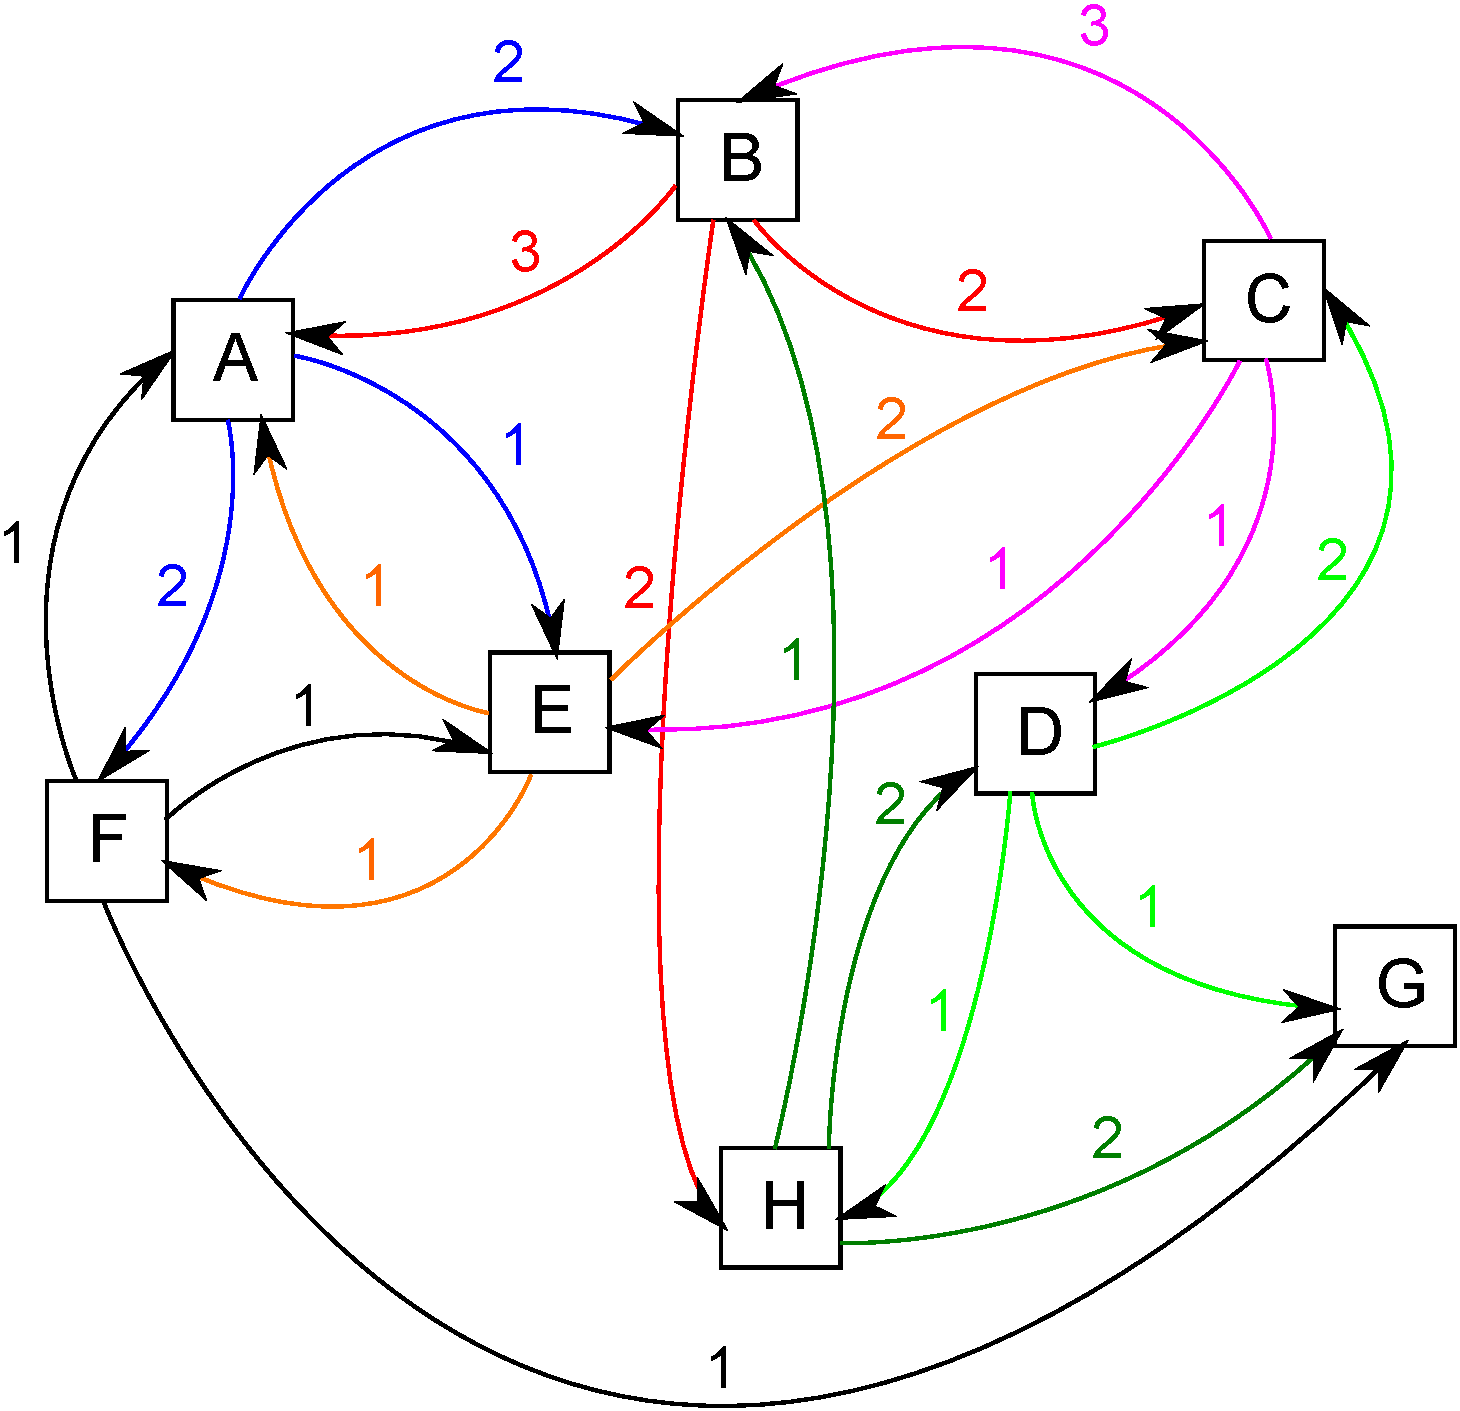
\includegraphics[width=8.0cm]{./images/zadanie05.pdf}
				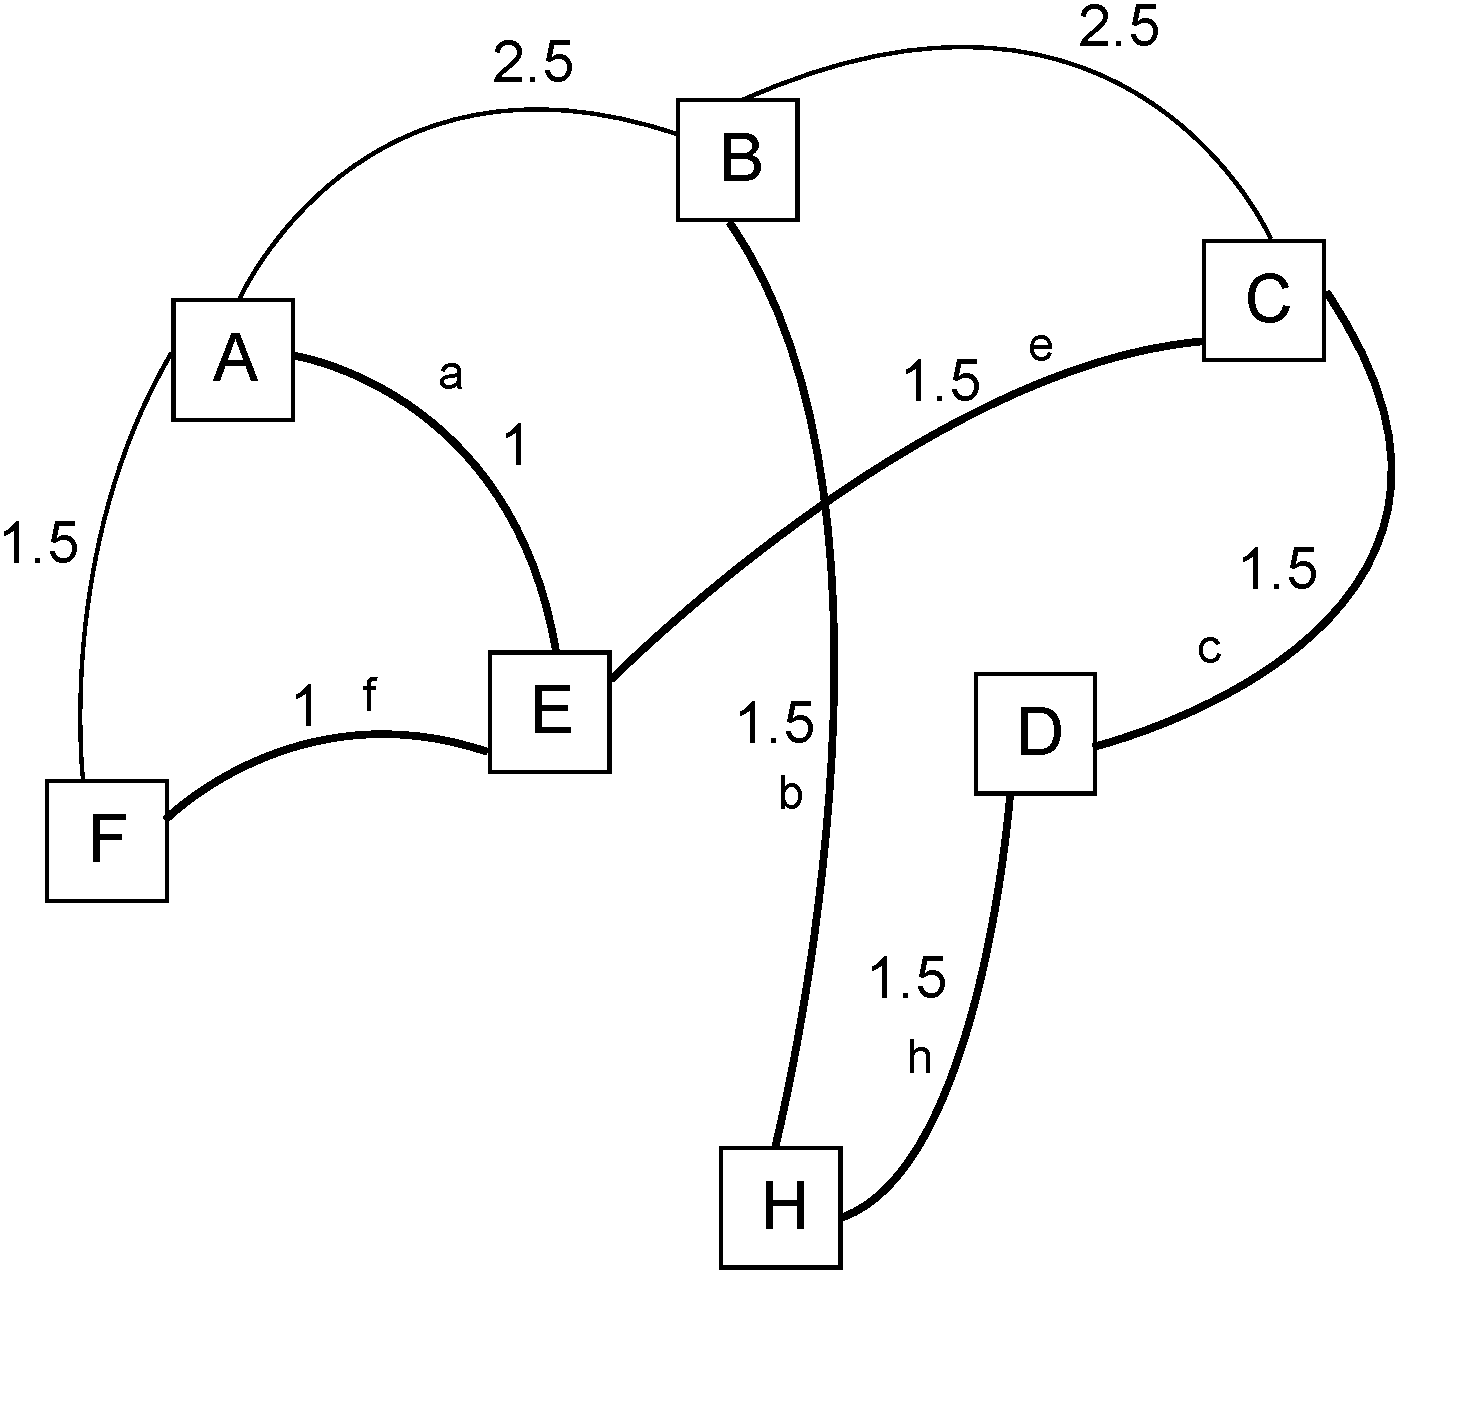
\includegraphics[width=8.0cm]{./images/zadanie06.pdf}\\
			Jeśli węzły da się połączyć na dwa różne sposoby, tworzymy średnią arytmetyczną. Wybieramy najkrótsze możliwe połączenie do każdego węzła, \textbf{pomijamy G}, i rysujemy tabelkę.\\\\ 
			\begin{tabular}{c|c|c}
				Cel & Koszt & Przez \\ \hline
				A   & 4     & E     \\
				B   & 3     & H     \\
				C   & 1.5   & D     \\
				D   & 0     &       \\
				E   & 3     & C     \\
				F   & 4     & E     \\
				G   & -     &       \\
				H   & 1.5   & D     
			\end{tabular}\\
			\small{ \emph{Forczu: ocenione na 1.0 / 1.0\\
					Podobno uwzględnienie G to 0.0 / 1.0}}.
	% ================= ZADANIE 4.5 ==================
	\subsection{Zadanie}
		\subsubsection{Treść}
			Węzeł K po restarcie wysłał do sąsiadów L, I, F swoją początkową tablicę routingu i otrzymał od nich ich tablice routingu. Wyznacz nową tablicę routingu węzła K.\\\\
			\begin{tabular}{cc m{1cm}|c|c|c|c|c|ccc}
				\cline{1-2} \cline{4-5} \cline{7-8} \cline{10-11}
				\multicolumn{2}{|c|}{\textbf{K}}                 &  & \multicolumn{2}{c|}{\textbf{L}} &  & \multicolumn{2}{c|}{\textbf{F}} & \multicolumn{1}{c|}{} & \multicolumn{2}{c|}{\textbf{I}}                 \\ \cline{1-2} \cline{4-5} \cline{7-8} \cline{10-11} 
				\multicolumn{1}{|c|}{I} & \multicolumn{1}{c|}{1} &  & D              & 3              &  & A              & 3              & \multicolumn{1}{c|}{} & \multicolumn{1}{c|}{J} & \multicolumn{1}{c|}{2} \\ \cline{1-2} \cline{4-5} \cline{7-8} \cline{10-11} 
				\multicolumn{1}{|c|}{F} & \multicolumn{1}{c|}{2} &  & C              & 4              &  & B              & 2              & \multicolumn{1}{c|}{} & \multicolumn{1}{c|}{H} & \multicolumn{1}{c|}{3} \\ \cline{1-2} \cline{4-5} \cline{7-8} \cline{10-11} 
				\multicolumn{1}{|c|}{L} & \multicolumn{1}{c|}{1} &  & G              & 2              &  & C              & 1              & \multicolumn{1}{c|}{} & \multicolumn{1}{c|}{N} & \multicolumn{1}{c|}{3} \\ \cline{1-2} \cline{4-5} \cline{7-8} \cline{10-11} 
				&                        &  & H              & 1              &  & E              & 2              & \multicolumn{1}{c|}{} & \multicolumn{1}{c|}{M} & \multicolumn{1}{c|}{4} \\ \cline{4-5} \cline{7-8} \cline{10-11} 
				&                        &  & N              & 2              &  & G              & 1              & \multicolumn{1}{c|}{} & \multicolumn{1}{c|}{E} & \multicolumn{1}{c|}{3} \\ \cline{4-5} \cline{7-8} \cline{10-11} 
				&                        &  & M              & 5              &  & J              & 2              &                       &                        &                        \\ \cline{4-5} \cline{7-8}
			\end{tabular}
		\subsubsection{Odpowiedź}
		\begin{wraptable}{l}{5.5cm}
			\begin{tabular}{c|c|c}
				Do & Przez & Koszt \\ \hline
				A  & F     & 5     \\
				B  & F     & 4     \\
				C  & F     & 3     \\
				D  & L     & 4     \\
				E  & F     & 4     \\
				F  & -     & 2     \\
				G  & L     & 3     \\
				H  & L     & 2     \\
				I  & -     & 1     \\
				J  & I     & 3     \\
				K  & -     & -     \\
				L  & -     & 1     \\
				M  & I     & 5     \\
				N  & L     & 3    
			\end{tabular}
		\end{wraptable}
		W tym wszystkim interesują nas tylko drogi lokalnie najbliższe - te z punktu widzenia węzła K i "ofert" dróg sąsiadów. Jeśli dwie drogi mają ten sam koszt to wybór powinien być obojętny. Sąsiedzi (L, I, D) mają się w końcowej tabeli również znajdować.\\
		\small{ \emph{Forczu: ocenione na 1.0 / 1.0}}.\\\\\\\\\\\\\\\\\\\\\\\\
		
\newpage
% ==================================================
% --- 5. TRANSMISJA DANYCH
% ==================================================
\section{Transmisja danych}
% ================= ZADANIE 5.1 ==================
	\subsection{Zadanie}
		\subsubsection{Treść}
			Stacja robocza połączona jest z serwerem łączem szeregowym o przepustowości 8 MBit/s, z bitową stopą błędów $ BER=2\cdot 10^{-5} $. Określić z jaką średnią szybkością transmisji danych protokołem TCP w wersji standardowej (\emph{plain vanilla}) można uzyskać jeśli uzgodniona maksymalna wielkość segmentu wynosi 768 B (ramki w łączu 832 B), wielkość danych odbiorcy wynosi 27 kB, czas $ RTT=40\;ms $.
		\subsubsection{Odpowiedź}
			Algorytm wykonywania zadań z przekłamaniem:
			\begin{enumerate}
				\item Obliczamy liczbę przekłamań w jednostce czasu jako odwrotność BERu:
				$ \cfrac{1}{BER} = \cfrac{1}{2\cdot 10^{-5}}=50000 \rightarrow$ - oznacza to, że 1 na 50k bitów jest przekłamany $ \rightarrow $ co 6250 bajt jest przekłamany.
				\item Następnie obliczamy ile ramek zostaje przekłamanych jako:
				$$ \cfrac{Odwrotnosc\;BERu}{Rozmiar\;ramki\;w\;laczu} $$
				W naszym przypadku jest to $ \cfrac{6250\;[B]}{832\;[B]}=7.51$
				\item Powyższy wynik oznacza, że 7 ramek zostało wysłanych poprawie, a 8 jest przekłamana. Czyli zakładamy, że \textbf{co 8 ramka} jest błędna (bierzemy sufit wyniku).
				\item Obliczamy liczbę ramek jaką można maksymalnie przesłać w jednym RTT jako:
				$$ \cfrac{Rozmiar\;okna}{Rozmiar\;ramki\;w\;laczu} $$
				Czyli u nas: $ \cfrac{27\:000}{832}\approx32 $
				\item Następnie stosujemy \textbf{metodę słupków} do wyznaczenia właściwego stosunku liczby ramek, jakie można wysłać.
				\begin{enumerate}
					\item Rysujemy kolejne transmitowane ramki w postaci słupków złożonych z $ 2^n $ ramek: 1, 2, 4, 8 itd.
					\begin{enumerate}
						\item Jeżeli protokół jest typu \emph{slow start} - naliczamy bezwzględnie wg $ 2^n $ - kolejne słupki mają 16, 32 itd. wysokości
						\item Jeżeli protokół jest typu \emph{congestion avoidance} - po przekroczeniu połowy okna zaczynamy zwiększać wysokość \textbf{liniowo}, czyli np. dla granicy (\emph{thresholdu}) 8 kolejne słupki będą mieć 9, 10, 11 itd. wysokości.
						\item \emph{congestion avoidance} wykorzystujemy, gdy w poleceniu mamy bufor (podobno).
					\end{enumerate}
					\item Gdy napotykamy przekłamaną ramkę zaczynamy naliczać od nowa.
					\item Liczba ramek w słupku nie może przekroczyć maksymalnej liczby ramek jaką można wysłać w czasie RTT.
					\item Kończymy naliczanie gdy przekłamana ramka znajdzie się na szczycie jednego ze słupków, czyli po zakończeniu jednego cyklu.
				\end{enumerate}
				\item Przystępując do rysowania słupków należy zaznaczyć jaki algorytm wybraliśmy. Niech będzie "slow start", ale podobno jest zalecany CA na examie.\\
				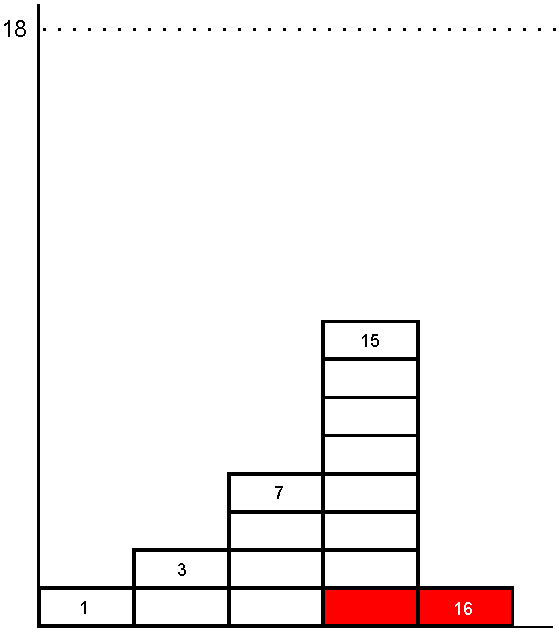
\includegraphics[width=6.0cm]{./images/zadanie07.pdf}\\\\
				Wynika z tego, że na 16 pakietów 2 zostają przekłamane. $ 16 - 2 = 14 $ - nieprzekłamane pakiety. Liczba ta nie powinna zostać przekroczona w wysyłaniu danych do okna.
				\item Na koniec pozostaje obliczyć efektywną prędkość. Może ona zostać obliczona wg dwóch wzorów:
				\begin{enumerate}
					\item \textbf{SRET}
					$$ SRET=\frac{((Liczba\;ramek - liczba\;ramek\;przekłamanych)\cdot Rozmiar\;segmentu}{Liczba\;kolumn\;w\;cyklu\cdot RTT} $$
					\item \textbf{GBN} - Go-Back-N
					$$ GBN=\frac{((Liczba\;ramek - (Ramki\;przekłamane + Ramki\;w\;slupkach\;ponad\;nimi))\cdot Rozmiar\;segmentu}{Liczba\;kolumn\;w\;cyklu\cdot RTT} $$
				\end{enumerate}
				\item W naszym zadaniu są to:
				$$ SRET=\frac{(16-2)\cdot 768\;[B]}{5\cdot 40\;[ms]}=\frac{14\cdot 768\;[B]}{5\cdot 40\;[ms]}=\frac{14\cdot 768\;[B]}{5\cdot 40\cdot 10^{-3}\;[s]}=53760\;[\frac{B}{s}]=52.5\; [\frac{kB}{s}]$$\\
				$$ GNB=\frac{(16-9)\cdot 768\;[B]}{5\cdot 40\;[ms]}=\frac{7\cdot 768\;[B]}{5\cdot 40\cdot 10^{-3}\;[s]}=26880\;[\frac{B}{s}]=26.25\;[\frac{kB}{s}] $$
			\end{enumerate}

	% ================= ZADANIE 5.2 ==================
	\subsection{Zadanie}
		\subsubsection{Treść}
			Stacja robocza połączona jest z serwerem łączem szeregowym o przepustowości $ 10\;Mbit/s $, z bitową stopą błędów $ BER=1.3\cdot 10^{-5} $. Określ z jaką średnią szybkością można przesyłać dane z serwera protokołem TCP w wersji standardowej, jeśli wielkość segmentu wynosi 768 B (ramki 832 B), wielkość okna odbiorcy 29 kB, średni czas $ RTT=45\;ms $.
		\subsubsection{Odpowiedź}
			\begin{enumerate}
				\item $ \cfrac{1}{1.3\cdot 10^{-5}}\approx 76\;923 $ - 1 bit na 76923 jest przekłamany, ok. 1 bajt na 9600 B.
				\item $ \cfrac{9600\:[B]}{832\:[B]}\approx11.54 $ - co 12 ramka jest przekłamana.
				\item $ \cfrac{29\;[kB]}{832\;[B]}=\cfrac{29\:000\;[B]}{832\;[B]}\approx 35 $ - tyle ramek można maksymalnie przesłać do okna.
			\end{enumerate}
			Ilustracja przekłamania ramek metodą słupków:\\\\
			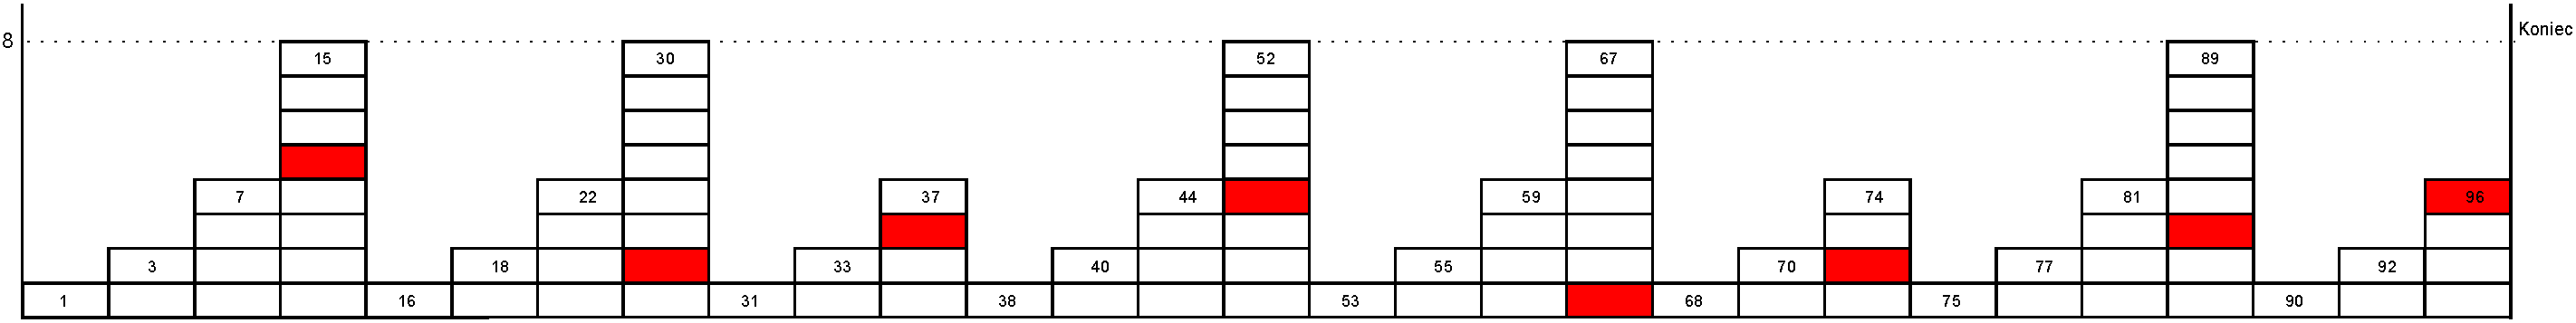
\includegraphics[width=16.0cm]{./images/zadanie08.pdf}\\\\
			Na 96 pakietów 8 zostaje przekłamanych.\\
			Możemy wyróżnić dwa parametry spełniające zadanie:
			\begin{enumerate}
				\item $$ SRET=\frac{(96-8)\cdot 768\;[B]}{29\cdot 45\;[ms]}=\frac{88\cdot 768\;[B]}{29\cdot 45\;[ms]} $$
				\item $$ GND=\frac{(96-36)\cdot 768\;[B]}{29\cdot 45\;[ms]}=\frac{60\cdot 768\;[B]}{29\cdot 45\;[ms]} $$
			\end{enumerate}
			\small{ \emph{Forczu: w tego typu zadaniach przepustowość chyba zawsze jest maksymalna, a protokoół standardowy, co ma upraszczać całość.
			Ktoś tam napisał, że wielkość ramki we wzorach jest obojętna, ale należy zaznaczyć, czy bierzemy dane czy dane + narzut.}}.
\newpage
	% ================= ZADANIE 5.3 ==================
	\subsection{Zadanie}
		\subsubsection{Treść}
			Stacja robocza podłączona jest z serwerem łączem Fast Ethernet o przepustowości $100\;Mbit/s $, z bitową stopą błędów $ BER=6.6\cdot 10^{-6} $. Uzgodniona wielkość segmentu to 1024 [B] (1088 [B] w łączu), wielkość okna odbiorcy wynosi 27 [kB], czas RTT wynosi 40 [ms]. Określić, ile czasu zajmie przesył 1 [MB] tym łączem protokołu TCP w wersji standardowej.
		\subsubsection{Odpowiedź}
		\begin{enumerate}
			\item $ \cfrac{1}{BER}=\cfrac{1}{6.6\cdot 10^{-6}}=151515$, co oznacza, że 1 na 151515 bitów jest przekłamany $ \rightarrow $ 1 na 18939 bajtów.
			\item $ \cfrac{18939\;[B]}{1\:088\;[B]}\approx17.41 \rightarrow $ co 18 ramka jest przekłamana.
			\item $ \cfrac{27\;[kB]}{1\:088\;[B]}=\cfrac{27\:000\;[B]}{1088\;[B]}=24.82 \rightarrow $, co oznacza maksymalnie 24 ramki w słupku.
			\item
				\begin{center}
					\includegraphics[width=9.0cm]{./images/zadanie14.pdf}
				\end{center}
			\item Odpowiedź
			$$ SRET=\cfrac{68\cdot1024\:[B]}{15\cdot40\:[ms]}=\approx113\;[\cfrac{kB}{s}]$$
			$$\\\\ GNB=\cfrac{38\cdot1024\:[B]}{15\cdot40\:[ms]}=\approx63\;[\cfrac{kB}{s}]$$
		\end{enumerate}
	% ================= ZADANIE 5.4 ==================
\newpage
	\subsection{Zadanie}
		\subsubsection{Treść}
			Użytkownik połączony jest z routerem łączem sieci lokalnej 10 Mbps Ethernet, czas RTT = 35 ms, router dostępowy na obsługę użytkownika przeznacza bufor 12 kB, rozmiar okna protokołu TCP = 27 kB. Określić maksymalną średnią szybkość transmisji możliwą do uzyskania przez użytkownika przez standardowej wersji protokołu TCP.
		\subsubsection{Odpowiedź}
			{\small \emph{Forczu: ponieważ w treści zadania jest podane, że mamy do czynienia z użytkownikiem łączącej się przez router z Internetem to WYDAJE MI SIĘ, że należy wykorzystać algorytm \emph{congestion avoidance}, który ma zastosowanie m.in. w przeglądarkach internetowych. Stąd ta różnica.}}\\
			\begin{enumerate}
				\item Ramka w Ethernecie: 1500 [B] (1460 [B] dla danych)
				\item W routerze jest dostępne 12000 [B].
				\item $ \cfrac{12\:000\;[B]}{1500\;[B]}=8 \rightarrow $ oznacza, że razem można wysłać 8 ramek, przy 9tej przepełni się bufor.
				\item \includegraphics[width=8.0cm]{./images/zadanie15.pdf}
				\item Na 24 ramki 1 została przekłamana. mamy więc 23 poprawne ramki oraz 5 słupków.
				\item $$ SRET=\cfrac{23\cdot1460\:[B]}{5\cdot35\:[ms]}=\cfrac{33580000\:[B]}{175\:[s]}=191885\:[\cfrac{B}{s}]=187\;[\cfrac{kB}{s}] $$
			\end{enumerate}
			
\newpage
	% ================= ZADANIE 5.5 ==================
	\subsection{Zadanie}
		\subsubsection{Treść}
			W systemie transmisji posługującym się protokołem SDLC / HDLC (tryb NRM, w=3, retransmisja grupowa) w łączu ze stopą błędów $ p=10^{-4} $ przesyłane są dane ramkami z polem danych 256 B, ze stacji nadrzędnej do stacji podrzędnej. Przedstaw przebieg transmisji w przesyle \textbf{4.5 kB} danych, pomiń nawiązanie / zrywanie połączenia. Ile kosztuje (narzut protokołu) obsługa błędów w transmisji?
		\subsubsection{Odpowiedź}
			Najpierw liczymy ilość potrzebnych ramek
			$$ \cfrac{4.5\;[kB]}{256\;[B]}=\cfrac{4\:500\;[B]}{256\;[B]}\approx17.58\;[ramek] $$Należy przesłać 18 ramek.\\
			Następnie należy wyliczyć, co którą ramkę pojawi się przekłamanie. Stopa błędu wynosi 1/10000, czyli to oznacza, że co 10000 bit następuje przekłamanie, co równa się 1250 B. Teraz należy obliczyć, co którą ramkę następuje błąd (i teraz nie jestem pewien ale chyba do tych 256 B danych należy dodać 6B nagłówka).
			$$ \cfrac{1250}{262}={4.77}\approx5 $$
			Co piąta ramka zawiera przekłamanie. Teraz można zacząć przedstawiać przebieg transmisji. "w" oznacza ile ramek możemy przesłać w takiej jednej sekwencji.
			\begin{center}
				\includegraphics[width=9.0cm]{./images/zadanie09.pdf}
			\end{center}
			Następnie należy policzyć narzut (ilość wszystkich ramek - ilość wymaganych ramek)\\
			$$ Narzut = 28 - 18  = 10\;ramek = 10 * 256\;B = 2560\;B =2,5\; [kB] $$
			\small{ \emph{Forczu: ocenione na 1.0 / 1.0}}.

\newpage
	% ================= ZADANIE 5.6 ==================
	\subsection{Zadanie}
		\subsubsection{Treść}
			W systemie z protokołem SDLC (tryb NRM, w=3, retransmisja grupowa), ze stopą błędów $ p=10^{-4} $, ramki są wysyłane z polem danych 256 B ze stacji nadrzędnej do podrzędnej. Przedstaw przebieg transmisji przy przesyle \textbf{4 kB} danych. Pomiń nawiązanie i zerwanie połączenia. Ile kosztuje (narzut protokołu) obsługa błędów w transmisji?
		\subsubsection{Odpowiedź}
			$ BER=p=10^{-4} \rightarrow$ 1 błąd co 10 000 bitów $ \rightarrow $ 1 błąd do 1250 bajów $ \rightarrow $ 1 błąd w przybliżeniu co 5 ramek.\\
			$$ \cfrac{4\;[kB]}{256\;[B]}=16\;[ramek] $$
			\begin{center}
				\includegraphics[width=8.0cm]{./images/zadanie10.pdf}
			\end{center}
			Wysłaliśmy łącznie 24 ramki. Narzut: 24 - 16 = 8 ramek = 2048 B = 2 kB
\newpage
	% ================= ZADANIE 5.7 ==================
	\subsection{Zadanie}
		\subsubsection{Treść}
			W systemie transmisji z protokołem HDLC średnio jeden na 9000 bitów jest przekłamany. Jaki będzie koszt obsługi błędów transmisji przy przesyle bloku 4 kB danych ze stacji B do stacji A w tym systemie, jeśli wielkość pola danych to 256 B, okno w=4, tryb NRM z retransmisją grupową.
		\subsubsection{Odpowiedź}
			$$ \cfrac{4\;[kB]}{256\;[B]}=16\;[ramek] $$
			Musimy przesłać 16 ramek.\\
			$ \cfrac{1}{9000} $ bitów przekłamanych $ \rightarrow \cfrac{1}{1125}\;[B] \rightarrow $ co 5 ramka przekłamana.\\\\
			\begin{center}
				\includegraphics[width=8.0cm]{./images/zadanie12.pdf}
			\end{center}
			Wysłano 28 ramek. Narzut: 28 - 16 = 12 ramek = 3072 B = 3 kB.
\newpage		
	% ================= ZADANIE 5.8 ==================
	\subsection{Zadanie}
		\subsubsection{Treść}
			Drukarka wierszowa posiada jeden bufor na 80 znaków (1 wiersz tekstu). Wydruk bufora zajmuje 25 ms, w czasie których drukarka nie przyjmuje danych. Stacja nadrzędna przesyła notatkę - 3 wiesze (bloki po 80 znaków) łączem o szybkości transmisji 19200 bitów / s, protokół BSC (2 znaki SYN). Przedstaw przebieg komunikacji SN-SP (drukarka). Załóż brak przekłamań, pomiń fazę nawiązania połączenia. Przyjmij czas przetwarzania żądania / odpowiedzi i propagacji sygnału łączem 2.5 $ \mu s $.
		\subsubsection{Odpowiedź}
		Jak mamy bufor to liczymy wg \emph{congestion avoidance}
			19200 $ [\cfrac{b}{s}] $ = 2400 $ [\cfrac{B}{s}] $, czyli 2.4k $ \cfrac{znakow}{s} $, ostatecznie ok. 0.4 ms na jeden znak.
			\begin{center}
				\includegraphics[width=16.0cm]{./images/zadanie13.pdf}
			\end{center}
			\begin{itemize}
				\item Sprowadzamy prędkość transmisji do czasu przesyłu jednego znaku: 1 znak / 0.4 ms. Jest to podstawa do większości czasów.
				\item Stacja nadrzędna, jak się połączy, zaczyna nadawać. Przesyłamy 80 znaków oraz 6 rozkazów. Drukarka odbiera i zaczyna drukować.
				\item Drukowanie ma trwać (minimum) 25 ms. W tym czasie drukarka wysyła WACKi - SN nie wysyła danych, ale zostaje utrzymana komunikacja. SN następnie wysyła zapytania ENQ - czy może przesłać następny wiersz.
				\item Drukarka kończy działanie po 4 wymianach jałowej informacji, po czym wysyła SYN SYN ACK. Po tym sygnale komputer może wysłać kolejne 80 znaków do drukarki. Aby wysłać kolejne 2 wiersze należy całość powtórzyć jeszcze 2 razy.
				\item Podobno swetrowi chodziło bardziej o zilustrowanie procesu niż wyliczania czasów.
			\end{itemize}
			
			
% ==================================================
% --- 6. ADRESACJA
% ==================================================
\newpage
\section{Adresacja}
	% ================= ZADANIE 6.1 ==================
	\subsection{Zadanie}
		\subsubsection{Treść}
			Jak przebiega (po raz pierwszy w danych środowisku) proces tłumaczenia nazwy na adres IP dla nazwy daisy.sales.euro.hp.com? Czy zwracany wynik i proces tłumaczenia różni się czymś przy drugiej próbie w stosunku do pierwszej (odstęp między żądaniami kilka minut, pierwsza zakończona pomyślnie)? Jak będzie przebiegał późniejszy o kilka minut proces tłumaczenia nazwy dino.support.americas.hp.com?
		\subsubsection{Odpowiedź}
			\begin{enumerate}[A]
				\item \includegraphics[width=6cm]{./images/zadanie01.pdf}\\
				\begin{enumerate}[1]
					\item Zapytanie DNS o adres IP dla daisy.sales...
					\item Jeśli DNS nie posiada tego adresu to pyta root server
					\item Ten odpowiada, że nie zna adresu IP dla daisy.sales.euro.hp.com , ale zna adres dla com i ... (przekierowuje)
					\item DNS ISP pyta dns com o daisy.sales.euro.hp.com
					\item Ten odpowiada, że go nie zna, ale zna adres dla hp
					\item DNS ISP pyta dns hp o daisy.sales.euro.hp.com
					\item Ten odpowiada, że go nie zna, ale zna adres dla euro
					\item DNS ISP pyta dns euro o daisy.sales.euro.hp.com
					\item Ten odpowiada, że go nie zna, ale zna adres dla sales
					\item DNS ISP pyta dns sales o daisy.sales.euro.hp.com
					\item Serwer sales zwraca adres IP domeny daisy.sales.euro.hp.com. Następnie DNS ISP p(...) go do hosta.
					\item ...
				\end{enumerate}
				\small{ \emph{Brak pełnej treści, ale ocenione na 1.0 / 1.0}}
				\item
					\begin{enumerate}
						\item daisy.sales.euro.hp.com.root
						\begin{enumerate}[1]
							\item Zapytanie do NS .com czy "zna" .hp
							\item Zapytanie do NS .hp czy zna .euro
							\item Zapytanie do NS .euro czy zna .sales
							\item Zapytanie do NS .sales czy zna .daisy
							\item Otrzymanie adresu IP
						\end{enumerate}
						W drugim przypadku adres hp.com może nie być tłumaczony.
						\item dino.support.americas.hp.com
						\begin{enumerate}[1]
							\item Znamy IP (hp.com), pytamy czy zna .americas
							\item Zapytanie do NS czy zna .support
							\item Zapytanie do NS czy zna .dino
							\item Otrzymanie adresu IP
						\end{enumerate}
					\end{enumerate}
					\small{ \emph{Ocenione na 1.0 / 1.0}}
			\end{enumerate}
	% ================= ZADANIE 6.2 ==================
	\subsection{Zadanie}
		\subsubsection{Treść}
			Dostępna jest pewna ilość kolejnych adresów internetowych, zaczynając od 192.170.0.0. Cztery organizacje A, B, C i D występowały kolejno o przydział puli 1000, 2000, 4000 i 1000 adresów IP. Podaj dla każdej z nich pierwszy i ostatni przyznany adres oraz maskę sieci w notacji w.x.y.z i /m.
		\subsubsection{Odpowiedź}
			W treści zadania jest podane, że te firmy przychodziły \textit{kolejno}, więc po prostu w tej kolejności przyznajemy im adresy.
			\begin{enumerate}
				\item Firma A, 1000 adresów - maska na 1024 adresy (niezbędne minimum), czyli odcinamy 10 bitów by utworzyć maskę:
				$$ 11111111.11111111.11111100.00000000=/22=255.255.252.0$$
				\begin{itemize}
					\item Pierwszy adres: 192.170.0.0
					\item Ostatni adres: 192.170.3.255
					\item w.x.y.z: 255.255.252.0
					\item Maska: /22
				\end{itemize}
				\item Firma B, 2000 adresów - maska na 2048 adresy.
				$$ 11111111.11111111.11111000.00000000=/21=255.255.248.0$$
				\begin{itemize}
					\item Nie możemy w połowie wstawić takiej maski, ponieważ wcześniej utworzyliśmy podsieć na 1024 adresy. Dlatego wymagana jest przerwa do uzupełnienia do 2048. Innymi słowy musimy zostawić przerwę po pierwszej podsieci o długości 1024 adresy, by wyrównać je.
					\item Pierwszy adres: 192.170.8.0
					\item Ostatni adres: 192.170.15.255
					\item w.x.y.z: 255.255.248.0
					\item Maska: /21
				\end{itemize}
				\item Firma C, 4000 adresów - maska na 4096 adresy.
				$$ 11111111.11111111.11110000.00000000=/20=255.255.240.0$$
				\begin{itemize}
					\item Tutaj nie musimy dokonywać analogicznego uzupełnienia. W dwóch poprzednich procesach łącznie przeszliśmy przez 4096 adresów, więc tę sieć możemy wstawić bezpośrednio za drugą.
					\item Pierwszy adres: 192.170.16.0
					\item Ostatni adres: 192.170.31.255
					\item w.x.y.z: 255.255.240.0
					\item Maska: /20
				\end{itemize}
				\item Firma D, 1000 adresów - maska na 1024 adresy
				\begin{itemize}
					\item Mamy wolne miejsce między podsieciami dla firmy A i B, tam dajemy tę sieć.
					\item Pierwszy adres: 192.170.4.0
					\item Ostatni adres: 192.170.7.255
					\item w.x.y.z: 255.255.252.0
					\item Maska: /22
				\end{itemize}
			\end{enumerate}
\newpage
	% ================= ZADANIE 6.3 ==================
	\subsection{Zadanie}
		\subsubsection{Treść}
			Firma dysponuje pulą 32 adresów IP. Przyjęto, że pierwszy i ostatni użyteczny adres zostaną przydzielone routerowi dostępowemu i serverowi DNS. Jeden z komputerów otrzymał adres 172.19.21.137. Podaj elementy konfiguracji IP tego komputera.
		\subsubsection{Odpowiedź}
			\begin{itemize}
				\item \textbf{Maska podsieci}: 255.255.255.224 (albo /27)\\
				Firma posiada 32 adresy, które różnią się 5 najmłodszymi bitami. 32 - 5 = 27.
				\item \textbf{Adres IP}: 172.19.21.137
				\item \textbf{Host}: 172.19.21.128 /27 (adres sieci)\\
				Adresem sieci wyliczamy zerując 5 ostatnich bitów. (albo ANDując adres z 1.1.1.11100000)
				\item \textbf{Brama / Router}: 172.19.21.129\\
				Adres routera dostępowego, pierwszy użyteczny adres (00001).
				\item \textbf{Serwer DNS}: 172.19.21.158\\
				Ostatni użyteczny adres (11110). (Broadcast - 1)
				\item \textbf{Broadcast}: 172.19.21.159\\
				Adres rozgłoszeniowy, uzyskany przez "zajedynkowanie" 5 ostatnich bitów. Największy adres w sieci.
				\item Adresy przydzielamy wg kolejnych potęg dwójki $ 2^n $. Gdyby w treści były 33 adresy, to przydzielalibyśmy 64.
				\item Gdyby w treści należałoby podpiąć 32 klientów, to musielibyśmy mieć 34 adresy i znów przydzielać 64.
			\end{itemize}
	% ================= ZADANIE 6.4 ==================
	\subsection{Zadanie}
		\subsubsection{Treść}
			Rekord SOA domeny abc.com zawiera następujące wartości:
			\begin{itemize}
				\item refresh = 10800
				\item retry = 5400
				\item expire = 86400
				\item default TTL = 7200
			\end{itemize}
			Administrator domeny zaplanował zastąpienie wysłużonego głównego \emph{name servera} nowym systemem (noy adres IP). Po jakim czasie (od dokonania zmiany rekordu NS) równoległej pracy obu \emph{name serverów} będzie można wyłączyć stary serwer.
		\subsubsection{Odpowiedź}	
			Po czasie TTL + refresh = 10 800 + 7200 = 18 000.
			
% ==================================================
% --- 7. POCZTA E-MAIL
% ==================================================
\newpage
\section{Poczta e-mail}
	% ================= ZADANIE 7.1 ==================
	\subsection{Zadanie}
		\subsubsection{Treść}
			Przedstawić z jakich elementów składa się koperta przesyłki poczty elektronicznej.
			\begin{enumerate}[a)]
				\item Jak przebiega i który z protokołów poczty elektronicznej odpowiada za jej przekazanie?
				\item Jak przebiega odbiór przesyłki przez adresata, który z protokołów obsługuje tę operację?
			\end{enumerate}
		\subsubsection{Odpowiedź}
			\begin{enumerate}[a)]
				\item List elektroniczny wysyłany jest za pomocą protokołu SMTP. Klient inicjuje połączenie poleceniem "helo". Następnie podaje adres nadawcy "mail from", adres odbiorcy "rcpt to", treść listu "data". 
				\\(Koniec części z danymi oznacza pusta linia z '.'. - \textit{doxus}) 
				\\Wiadomość kończy poleceniem "quit".
				\item Listy odbierane są za pomocą protokołów POP3. Klient żąda listy wiadomości poleceniem "list". Następnie pobiera cały żądany list i usuwa go z serwera : "Retr" i "Dele". Sesja kończy się poleceniem "quit". Oczywiście zanim to wszystko nastąpi musi zostać przeprowadzona autentyfikacja. Klient POP3 zaczyna sesję od podania nazwy użytkownika "user" i hasła "pass".
			\end{enumerate}
			\small{ \emph{Ocenione na 1.0 / 1.0}}
	
	% ================= ZADANIE 7.2 ==================
	\subsection{Zadanie}
		\subsubsection{Treść}
			Przesyłka e-mail zawiera fragment tekstu: "płoną góry, płoną lasy..." . Przedstaw sposób zakodowania pierwszych słów treści listu zapewniający (dowolnym łączem) poprawny przesył znaków narodowych.
		\subsubsection{Odpowiedź}
			Zastosowany algorytm to QPE (\emph{Quoted Printable Encoding}). Treść wiadomości:
			\begin{center}
				p\textbf{=B3}on=B9 g\textbf{=F3}ry, p\textbf{=B3}on\textbf{=B9} lasy
			\end{center}
			Gdzie:
			\begin{itemize}
				\item =B3 - dziesiętnie 179 - ł w ASCII
				\item =B9 - dziesiętnie 185 - ą w ASCII
				\item =F3 - dziesiętnie 243 - ó w ASCII
			\end{itemize}
			Dziesiętne kody w ASCII były podane w poleceniu, należało je zmienić na zapis szesnastkowy.
			


% === SŁOWNIK
% !TeX spellcheck = pl_PL
\newcommand{\elementPL}[2]{\textbf{#1} - #2}
\newcommand{\elementANG}[2]{\textbf{#2} - #1}

\newpage
\part{Słownik pojęć sieciowych}

\section{Słownik angielsko-polski}
	\subsection{Podstawy}
		\begin{enumerate}
			\item \elementPL{Binary Synchronous Communication}{Binarna komunikacja synchroniczna}
			\item \elementPL{Confirmation}{Potwierdzenie}
			\item \elementPL{Connection}{Połączenie}
			\item \elementPL{Destination Address}{Adres przeznaczenia}
			\item \elementPL{Digital device}{Jednostka cyfrowa}
			\item \elementPL{Encapsulation}{Enkapsulacja}
			\item \elementPL{Encryption}{Szyfrowanie}
			\begin{enumerate}
				\item \elementPL{Application}{Warstwa aplikacyjna}
				\item \elementPL{Presentation}{Warstwa prezentacyjna}
				\item \elementPL{Session}{Warstwa sesji}
				\item \elementPL{Transport}{Warstwa transportowa}
				\item \elementPL{Network}{Warstwa sieci}
				\item \elementPL{Link Access}{Warstwa łącza danych}
				\item \elementPL{Physical Access}{Warstwa fizyczna}
			\end{enumerate}
			\item \elementPL{File transfer}{Transport plików}
			\item \elementPL{Finite-State Machine}{Automat stanów skończonych}
			\item \elementPL{Flag}{Flaga}
			\item \elementPL{Frame}{Ramka}
			\item \elementPL{Framing}{Ramkowanie}
			\item \elementPL{Header}{Nagłówek}
			\item \elementPL{Host}{Stacja}
			\item \elementPL{Layer}{Warstwa}
			\item \elementPL{Link}{Łącze}
			\item \elementPL{Message}{Komunikat}
			\item \elementPL{Network}{Sieć}
			\item \elementPL{Package}{Pakiet}
			\item \elementPL{Party}{Stacja}
			\item \elementPL{Preamble}{Preambuła}
			\item \elementPL{Receive}{Odbiór}
			\item \elementPL{Remote}{Zdalny}
			\item \elementPL{Send}{Nadanie}
			\item \elementPL{Source Address}{Adres źródłowy}
			\item \elementPL{Token}{Żeton}
		\end{enumerate}
	\subsection{Transfery}
		\begin{enumerate}
			\item \elementPL{Broadcast Transfer}{Transmisja rozgłoszeniowa}
			\item \elementPL{Full two-way service}{Pełny Dwukierunkowy Transfer}
			\item \elementPL{Half-duplex Transfer}{Jednokierunkowy Transfer Danych}
			\item \elementPL{Reliable Data Transfer}{Niezawodny Transfer Danych}
			\item \elementPL{Sliding Window}{Przesuwne Okno}
		\end{enumerate}
	\subsection{Algorytmy}
		\begin{enumerate}
			\item \elementPL{Go-Back-N}{Cofnij się o N}
		\end{enumerate}
	\subsection{Błędy}
		\begin{enumerate}
			\item \elementPL{Bit Error Rate}{Stopa błędów bitu}
			\item \elementPL{Frame Error Rate}{Stopa błędów ramek}
		\end{enumerate}
	\subsection{Dostęp do łącza (Protokoły MAC)}
		\begin{enumerate}
			\item \elementPL{Open Access}{Swobodny dostęp}
			\item \elementPL{Partial / Medium Control Access}{Częściowo kontrolowany dostęp}
			\item \elementPL{Full Control Access}{Kontrolowany dostęp}
			\item \elementPL{Token Hold Timer (THT)}{Maksymalny czas przetrzymania Tokenu}
			\item \elementPL{Not Token Timer (NTT)}{Czas czekania na token}
		\end{enumerate}
	\subsection{Rodzaje sieci}
		\begin{enumerate}
			\item \elementPL{Cambridge Ring}{Sieć typu Cambridge (chyba)}
			\begin{enumerate}
				\item \elementPL{Spanning Tree Protocol}{Protokół drzewa rozpinanego}
			\end{enumerate}
			\item \elementPL{Token Ring}{Sieć pierścieniowa}
		\end{enumerate}
	\subsection{Tryb pracy sieci}
		\begin{enumerate}
			\item \elementPL{Channel switching}{Komutacja kanałów}
			\item \elementPL{Information switching}{Komutacja informacji}
			\begin{enumerate}
				\item \elementPL{Information switching}{Komutacja wiadomości}
				\item \elementPL{Packet switching}{Komutacja pakietów}
			\end{enumerate}
		\end{enumerate}
	\subsection{Routing}
		\begin{enumerate}
			\item \elementPL{Routing}{Wybór drogi}
			\begin{enumerate}
				\item \elementPL{Source routing}{Routing źródłowy}
				\item \elementPL{Static routing}{Algorytm stałego wyboru}
				\item \elementPL{Adaptive routing}{Algorytm adaptacyjny}
				\begin{enumerate}
					\item \elementPL{Back learning}{Uczenie zwrotne}
					\item \elementPL{Cooperation routing}{Algorytm kooperacji}
				\end{enumerate}
			\end{enumerate}
			\item \elementPL{Broadcast}{Zalewanie}
			\item \elementPL{Hot potato}{Algorytm gorącego ziemniaka}
		\end{enumerate}
	\subsection{Obciążenie}
		\begin{enumerate}
			\item \elementPL{Random Error Discard/Detection}{Algorytm wyrzucania losowych pakietów}
			\item \elementPL{Error Recovery}{algorytm retransmisji}
		\end{enumerate}





\section{Słownik polsko-angielski}
	\subsection{Podstawy}
		\begin{enumerate}
			\item \elementANG{Finite-State Machine}{Automat stanów skończonych}
			\item \elementANG{Binary Synchronous Communication}{Binarna komunikacja synchroniczna}
			\item \elementANG{Destination Address}{Adres przeznaczenia}
			\item \elementANG{Source Address}{Adres źródłowy}
			\item \elementANG{Encapsulation}{Enkapsulacja}
			\begin{enumerate}
				\item \elementANG{Application}{Warstwa aplikacyjna}
				\item \elementANG{Presentation}{Warstwa prezentacyjna}
				\item \elementANG{Session}{Warstwa sesji}
				\item \elementANG{Transport}{Warstwa transportowa}
				\item \elementANG{Network}{Warstwa sieci}
				\item \elementANG{Link Access}{Warstwa łącza danych}
				\item \elementANG{Physical Access}{Warstwa fizyczna}
			\end{enumerate}
			\item \elementANG{Flag}{Flaga}
			\item \elementANG{Digital Device}{Jednostka cyfrowa}
			\item \elementANG{Message}{Komunikat}
			\item \elementANG{Link}{Łącze}
			\item \elementANG{Header}{Nagłówek}
			\item \elementANG{Receive}{Odbiór}
			\item \elementANG{Package}{Pakiet}
			\item \elementANG{Connection}{Połączenie}
			\item \elementANG{Confirmation}{Potwierdzenie}
			\item \elementANG{Preamble}{Preambuła}
			\item \elementANG{Frame}{Ramka}
			\item \elementANG{Framing}{Ramkowanie}
			\item \elementANG{Send}{Nadanie}
			\item \elementANG{Network}{Sieć}
			\item \elementANG{Party}{Stacja}
			\item \elementANG{Host}{Stacja}
			\item \elementANG{Encryption}{Szyfrowanie}
			\item \elementANG{Layer}{Warstwa}
			\item \elementANG{Remote}{Zdalny}
			\item \elementANG{Token}{Żeton}
		\end{enumerate}
	\subsection{Transfery}
		\begin{enumerate}
			\item \elementANG{Half-duplex Transfer}{Jednokierunkowy Transfer Danych}
			\item \elementANG{Reliable Data Transfer}{Niezawodny Transfer Danych}
			\item \elementANG{Full two-way service}{Pełny Dwukierunkowy Transfer}
			\item \elementANG{Sliding Window}{Przesuwne Okno}
			\item \elementANG{Broadcast Transfer}{Transmisja rozgłoszeniowa}
		\end{enumerate}
	\subsection{Algorytmy}
		\begin{enumerate}
			\item \elementANG{Go-Back-N}{Cofnij się o N}
		\end{enumerate}
	\subsection{Dostęp do łącza (Protokoły MAC)}
		\begin{enumerate}
			\item \elementANG{Open Access}{Swobodny dostęp}
			\item \elementANG{Partial / Medium Control Access}{Częściowo kontrolowany dostęp}
			\item \elementANG{Full Control Access}{Kontrolowany dostęp}
			\item \elementANG{Token Hold Timer (THT)}{Maksymalny czas przetrzymania Tokenu}
			\item \elementANG{Not Token Timer (NTT)}{Czas czekania na token}
		\end{enumerate}
	\subsection{Rodzaje sieci}
		\begin{enumerate}
			\item \elementANG{Token Ring}{Sieć pierścieniowa}
			\item \elementANG{Cambridge Ring}{Sieć typu Cambridge (chyba)}
			\begin{enumerate}
				\item \elementANG{Spanning Tree Protocol}{Protokół drzewa rozpinanego}
			\end{enumerate}
		\end{enumerate}
	\subsection{Tryb pracy sieci}
		\begin{enumerate}
			\item \elementANG{Channel switching}{Komutacja kanałów}
			\item \elementANG{Information switching}{Komutacja informacji}
			\begin{enumerate}
				\item \elementANG{Information switching}{Komutacja wiadomości}
				\item \elementANG{Packet switching}{Komutacja pakietów}
			\end{enumerate}
		\end{enumerate}
	\subsection{Obciążenie}
		\begin{enumerate}
			\item \elementANG{Random Error Discard/Detection}{Algorytm wyrzucania losowych pakietów}
			\item \elementANG{Error Recovery}{algorytm retransmisji}
		\end{enumerate}

\end{document}